% !TeX document-id = {a7b93078-8e1a-4028-b084-bf1785bdb871}
%%
% The BIThesis Template for Graduate Thesis
%
% Copyright 2020-2023 Yang Yating, BITNP
%
% This work may be distributed and/or modified under the
% conditions of the LaTeX Project Public License, either version 1.3
% of this license or (at your option) any later version.
% The latest version of this license is in
%   https://www.latex-project.org/lppl.txt
% and version 1.3 or later is part of all distributions of LaTeX
% version 2005/12/01 or later.
%
% This work has the LPPL maintenance status `maintained'.
%
% The Current Maintainer of this work is Feng Kaiyu.
%
% Compile with: xelatex -> biber -> xelatex -> xelatex

% !TeX program = xelatex
% !BIB program = biber

% 硕士论文模板 type=master
% 博士论文模板 type=doctor
% 开启盲审格式 blindPeerReview=true (如:[type=master,blindPeerReview=true])
% 开启双面打印模式 twoside=true (如:[type=master,twoside=true])
%     在双面打印模式下,需要放在奇数页的页面后会自动插入一个空白页,以方便直接在打印机上“双面打印”。
%
% 在 Linux 和 macOS 系统下,由于版权问题,中文字体和 Windows 系统下的字体不同。
% 如果想要获得与 Word 文档相同的效果,你有两个选择:
% 1. 使用 Windows 系统编译最终的论文。
% 2. 自己手动安装中易字库并添加选项:`\documentclass[...,ctex={fontset=windows}]{bithesis}`。
%
% **更多使用说明请参考 bithesis.pdf **

\documentclass[type=master,twoside=false,blindPeerReview=false]{bithesis}

% 此处仅列出常用的配置。全部配置用法请见「bithesis.pdf」手册。
\BITSetup{
  cover = {
    %% 使用以下参数来自定义封面日期
    date = 2025年6月,
    autoWidthPadding = 0.25em,
  },
  info = {
    % 想要删除某项封面信息,直接删除该项即可。
    % 想要让某项封面信息留空(但是保留下划线),请传入空白符组成的字符串,如"{~}"。
    % 如需要换行,则用 “\\” 符号分割。
    classification = TP311.5,
    UDC = 004.41,
    title = 基于强化学习的对抗性恶意软件生成技术研究,
    % 如需覆盖竖排标题,请配置以下选项。
    % 下面的例子展示了如何在竖排标题中使用垂直或者旋转的英文。
    % verticalTitle = {形状记忆聚氨酯{L } {T } {X }的合成 \rotatebox[origin=c]{-90}{Feng Kaiyu} 及其在织物中的应用},
    titleEn = {Research on adversarial malware generation technology based on reinforcement learning},
    author = 邓永琪, 
    authorEn = Yongqi Deng,
    studentId = 3220221018,
    school = 计算机学院,
    schoolEn = Computer Technology,
    supervisor = 邸慧军副教授,  % 指导教师
    supervisorEn = Associate Prof. Huijun Di,
    chairman = 危胜军副教授,  % 答辩委员会主席
    chairmanEn = Associate Prof. Shengjun Wei,
    % -------------
    % 请按自身研究生类型填写以下项目
    %
    % --- 学术型 ---
    % degreeType = academic,
    % degree = 工学博士,  % 申请学位
    % degreeEn = Doctor of Engineering,
    %major = 材料科学与工程,  % 一级学科
    % majorEn = Materials Science and Engineering,
    %
    % --- 专业型 ---
    degreeType = professional,
    industrialMentor = 彭武研究员,  % 行业合作导师
    industrialMentorEn = Researcher Wu Peng,
    degree = 工程硕士,  % 申请类别
    degreeEn = { Master of Engineering},
    major = 计算机技术,  % 学位领域
    majorEn = Computer Technology,
    % -------------
    %
    % 如果想要手动控制盲审模式下的隐藏信息,可以使用宏 \SecretInfo{}。使用方式有两种,如:
    % major = \SecretInfo{材料科学与工程} 可以得到 ******* (用等量的替换符号替代)
    % major = \SecretInfo{材料科学与工程}[ABCDEF] 可以得到 ABCDEF (用你自定义的内容替代)
    %
    defenseDate = 2025年6月,
    defenseDateEn = {June, 2025},
    keywords = {强化学习;对抗性样本生成;LSTM;ELF;动态奖励函数},
    keywordsEn = Reinforcement Learning; Adversarial Sample Generation; LSTM; ELF;  Dynamic Reward Function
    %
    % 必要时置于封面右上角,并按照国家规定进行标记。
    % classifiedLevel = 密级\BigStar 保密期限,
    %
    % 特别类型——工程硕博士专项
    % 工程硕博士专项 = true,
    % 特别类型——交叉研究方向(一般不用勾选)
    % crossResearch = true,
    % 特别类型——政府项目留学生(一般不用勾选)
    % internationalStudentUGP = true,
    % 以上三个选项不勾选时将会隐藏显示。
  },
  % 在目录页中不显示摘要和主要符号对照表的标题。
  TOC = {
    abstract = false,
    abstractEn = false,
    symbols = false,
  },
  style = {
    pageVerticalAlign = top,
    % 开启 Windows 平台下的中易宋体伪粗体。
    % windowsSimSunFakeBold = true,
    % 开启该选项后,将用 Times New Roman 的开源字体 TeX Gyre Termes 作为正文字体。
    % 这个选项适用于以下情况:
    % 1. 不想在系统中安装 Times New Roman。
    % 2. 在 Linux/macOS 下遇到 `\textsc` 无法正常显示的问题。
    % betterTimesNewRoman = true,
  },
  publications = {
    % 以下两个选项将影响「攻读学位期间发表论文与研究成果清单」中名称列表的省略阈值。
    % 一般来说,如果你在全部文献中最低排在第四位,建议你将两个值都设置为大于等于 4 的值。
    % 更详细的说明请见手册。
    maxbibnames = 10,
    minbibnames = 10,
    % 「攻读学位期间发表论文与研究成果清单」默认按学校要求,“按发表的时间顺序列出”。
    % 如需调整,可修改以下选项,详见 https://bithesis.bitnp.net/faq/bib-sort.html
    % sorting = false
  },
  % 采用章节标题级别的附录格式
  appendices / chapterLevel = true,
  const = {
    % 关于题名页的字段名称,截至2025年三月末,以下几项规定不完全一致:
    %     Word 模板(学位论文模版-{学术型,专业型}-2025.doc)、研函〔2018〕60号《北京理工大学研究生学位论文撰写规范》、GB/T 7713.1—2006《学位论文编写规则》
    % 目前的默认值按照 Word 模板,可能需要手动调整。
    % 例如取消注释下一行,会将「申请学位/类别」改为「申请学位级别」。
    % info / degree = {申\hspace{0.45ex}请\hspace{0.45ex}学\hspace{0.45ex}位\hspace{0.45ex}级\hspace{0.45ex}别},
    % 详见 https://bithesis.bitnp.net/faq/edit-const.html
  },
  misc = {
    % 关闭后,链接会用多种颜色表示,便于检查。
    % 无论是否开启,都不会影响打印效果。
    hideLinks = true,
    % 微调表格行间距
    tabularRowSeparation = 1.6,
  }
}

% 大部分关于参考文献样式的修改,都可以通过此处的选项进行配置。
% 详情请搜索「biblatex-gb7714-2015 文档」进行阅读。
\usepackage[
  defernumbers=true,
  backend=biber,
  style=gb7714-2015,
  gbalign=gb7714-2015,
  gbnamefmt=lowercase,
  gbpub=false,
  gbannote=true,
  gbpunctin=false,
  doi=false,
  url=false,
  eprint=false,
  isbn=false,
]{biblatex}

% 添加参考文献
\addbibresource{reference/main.bib}
% 攻读学位期间发表论文与研究成果清单,详细使用方法见 `chapters/pub.tex`。
\addbibresource{reference/pub.bib}

\usepackage{enumitem}
\usepackage{graphicx}
\usepackage{algpseudocode}
\usepackage[linesnumbered,ruled,vlined]{algorithm2e}
\usepackage{float}
\usepackage{comment}
\usepackage{array}





\begin{document}

% 封面绘制
\MakeCover

% 打印书脊
\MakePaperBack

% 中文信息与英文信息
\MakeTitle

% 论文原创性声明和使用授权
\MakeOriginality

%%%%%%%%%%%%%%%%%%%%%%%%%%%%%%
%% 前置部分
%%%%%%%%%%%%%%%%%%%%%%%%%%%%%%
\frontmatter

% 摘要
%%
% The BIThesis Template for Graduate Thesis
%
% Copyright 2020-2023 Yang Yating, BITNP
%
% This work may be distributed and/or modified under the
% conditions of the LaTeX Project Public License, either version 1.3
% of this license or (at your option) any later version.
% The latest version of this license is in
%   https://www.latex-project.org/lppl.txt
% and version 1.3 or later is part of all distributions of LaTeX
% version 2005/12/01 or later.
%
% This work has the LPPL maintenance status `maintained'.
%
% The Current Maintainer of this work is Feng Kaiyu.
\begin{abstract}
 随着互联网技术的迅猛发展及其广泛应用,各类软件如雨后春笋般层出不穷,软件格式也日益多样化。这些软件在为人们的日常生活与工作带来便捷的同时,也带来了新的网络安全隐患。不法分子将恶意代码伪装成正常应用程序,巧妙绕过主机安全防护机制,潜入用户终端,从而窃取隐私信息、敏感数据,甚至控制系统资源,给用户带来严重损失。
 
 面对日益复杂与隐蔽的恶意软件威胁,研究人员不断探索与创新,提出了多种检测技术。然而,网络安全始终是一个“攻防对抗”的动态博弈过程。为应对日趋频繁的零日攻击和高级持续性威胁(APT),越来越多的研究者开始聚焦于对抗性技术,探索如何生成具备逃避检测能力的恶意样本。
 
 近年来,基于强化学习的对抗样本生成方法逐渐成为研究热点,尽管已有一些成果,但当前大多数方法仍存在针对单一检测模型、扰动操作粗糙、缺乏对恶意行为语义理解等问题。尤其是在扰动策略上,多采用随机字节插入,导致扰动缺乏语义性和隐蔽性,影响样本的可用性与逃避能力。
 
 为此,本文提出并设计了一种基于强化学习的多维度对抗性恶意软件生成框架。该框架从结构层、指令层与行为层三个维度对原始恶意样本进行扰动修改,区别于传统方法中插入随机字节的做法,本文创新性地引入良性样本中的字节作为扰动来源,使得生成的对抗样本在语义上更具合理性,扰动更加隐蔽,有效提升逃避检测系统的能力。
 
 在强化学习环境设计方面,本文构建了支持多维扰动操作的仿真环境,并采用PPO算法结合LSTM网络结构,充分挖掘扰动序列之间的潜在关联,提升扰动的语义一致性与时序依赖建模能力。此外,针对实际应用中对资源的敏感性,本文引入动态奖励函数机制,综合考虑扰动代价与训练效率,优化生成策略以提升样本的实用性与通用性。
 
 实验结果表明,该方法不仅能够成功绕过多种主流恶意软件检测系统,还展现出较强的迁移能力,能够有效对抗主流检测模型,具有良好的研究价值与实际应用前景。
\end{abstract}

% 如需手动控制换行连字符位置,可写 aa\-bb,详见
% https://bithesis.bitnp.net/faq/hyphen.html

\begin{abstractEn}
  
  With the rapid development and widespread application of Internet technologies, a wide variety of software programs have emerged like mushrooms after the rain, and software formats have become increasingly diverse. While these applications bring convenience to people’s daily lives and work, they also introduce new cybersecurity risks. Malicious actors disguise harmful code as legitimate applications to cleverly bypass host security mechanisms, infiltrate user terminals, steal private and sensitive data, and even take control of system resources, causing severe damage to users.

  In response to increasingly complex and stealthy malware threats, researchers have continuously explored and proposed a variety of detection technologies. However, cybersecurity remains a dynamic "cat-and-mouse" game between attack and defense. To counter frequent zero-day attacks and advanced persistent threats (APTs), an increasing number of researchers have turned their attention to adversarial techniques, exploring how to generate malicious samples capable of evading detection.
  
  In recent years, adversarial malware generation methods based on reinforcement learning have gradually become a research hotspot. Although some achievements have been made, most current approaches still suffer from several limitations, such as targeting only a single detection model, employing coarse-grained perturbations, and lacking an understanding of the semantic behavior of malware. In particular, many methods rely on inserting random bytes as perturbations, which undermines the semantic relevance and stealthiness of the modifications, thereby compromising both usability and evasiveness.
  
  To address these issues, this paper proposes and designs a multi-dimensional adversarial malware generation framework based on reinforcement learning. The framework perturbs original malware samples from three dimensions: structural, instruction-level, and behavioral. Unlike traditional methods that insert random bytes, this study innovatively uses bytes from benign samples as the source of perturbation, enhancing the semantic validity and stealthiness of the adversarial samples and significantly improving their ability to evade detection.
  
  For the reinforcement learning environment, we construct a simulation environment that supports multi-dimensional perturbation operations and employ the PPO (Proximal Policy Optimization) algorithm combined with an LSTM network to fully capture potential correlations in the perturbation sequences. This enhances semantic consistency and models temporal dependencies more effectively. Additionally, considering the resource constraints in practical applications, a dynamic reward function mechanism is introduced to balance perturbation cost and training efficiency, thereby optimizing the generation strategy to improve the practicality and generalizability of the samples.
  
  Experimental results demonstrate that the proposed method not only successfully evades various mainstream malware detection systems but also exhibits strong transferability across detection models, showing significant research value and promising real-world application prospects.
\end{abstractEn}



% 制作目录
\MakeTOC

% 插图目录
\listoffigures
% 表格目录
\listoftables

% 主要符号对照表
%%%
% The BIThesis Template for Graduate Thesis
%
% Copyright 2020-2023 Yang Yating, BITNP
%
% This work may be distributed and/or modified under the
% conditions of the LaTeX Project Public License, either version 1.3
% of this license or (at your option) any later version.
% The latest version of this license is in
%   https://www.latex-project.org/lppl.txt
% and version 1.3 or later is part of all distributions of LaTeX
% version 2005/12/01 or later.
%
% This work has the LPPL maintenance status `maintained'.
%
% The Current Maintainer of this work is Feng Kaiyu.

\begin{symbols}
  \item[BIT] 北京理工大学的英文缩写
  \item[\LaTeX] 一个很棒的排版系统
  \item[\LaTeXe] 一个很棒的排版系统的最新稳定版
  \item[ctex] 成套的中文\LaTeX{}解决方案,由一帮天才们开发
  \item[$ e^{\pi{}i}+1=0$] 一个集自然界五大常数一体的炫酷方程
\end{symbols}


\mainmatter

% 请根据论文内容,按照顺序添加章节。
%%%
% The BIThesis Template for Graduate Thesis
%
% Copyright 2020-2023 Yang Yating, BITNP
%
% This work may be distributed and/or modified under the
% conditions of the LaTeX Project Public License, either version 1.3
% of this license or (at your option) any later version.
% The latest version of this license is in
%   https://www.latex-project.org/lppl.txt
% and version 1.3 or later is part of all distributions of LaTeX
% version 2005/12/01 or later.
%
% This work has the LPPL maintenance status `maintained'.
%
% The Current Maintainer of this work is Feng Kaiyu.
\chapter{绪论 Introduction}

\label{chap:intro}
\section{研究的目的和意义 Purpose and Significance of This Research}

随着数字化、网络化、智能化技术的快速推进,全球网络空间正以前所未有的速度拓展,软件已渗透到政府管理、社会服务、产业控制、个人生活等各个层面。然而,软件的快速迭代与大规模部署在带来便利的同时,也使其成为网络攻击的重点目标。软件安全问题日益突出,恶意软件成为网络攻击中最活跃、最隐蔽、危害最大的武器之一,对国家安全、经济发展乃至社会稳定都构成了严重威胁。

With digitalization, networking, and artificial intelligence technologies developing rapidly, global cyberspace is expanding at an unprecedented pace. Software has permeated every layer of government administration, social services, industrial control, and personal life. However, the rapid iteration and large-scale deployment of software not only reveals that software brings convenience, but also implies that the software has also been a prime target for cyberattacks. Software security issues which pose a serious threat to national security, economic development, and even social stability have been more and more prominent, with the severe condition that malicious software emerges as one of weapons which is the most active, covert, and damaging in cyberattacks.

据《Security Navigator 2024》报告显示,2023年全球网络安全形势持续严峻,Orange Cyberdefense CyberSOC共检测129,395起网络攻击事件,同比增长30\%。其中,被安全分析师确认具有实际威胁的安全事件达25,076起,黑客攻击、权限滥用与恶意软件攻击占据主导地位。报告指出,2023年全球勒索软件受害者数量创下历史新高,同比激增46\%;政府机关、能源、电力、医疗等关键基础设施成为高级持续性威胁(APT)攻击的重点目标,呈现出“定向性强、潜伏时间长、破坏力大”的特点\cite{securitynavigator2024}。

The Security Navigator 2024 report reveals the fact that the global cybersecurity condition continued to be severe in 2023. Orange Cyberdefense's CyberSOC detected 129,395 cyberattack incidents, which represents an increase of 30\% compared to last year. Among these, security analysts confirmed 25,076 incidents that are dominated by hacker attacks, privilege abuse, and malicious software attacks result in actual threats. The report highlighted that the number of global ransomware victims reached a historic high in 2023, which surges 46\% compared to last year. Critical infrastructure sectors such as government agencies, energy, power, and healthcare became primary targets for Advanced Persistent Threat (APT) attacks, which are characterized as being highly targeted, long-dormant, and highly destructive.\cite{securitynavigator2024}

2025年2月,奇安信威胁情报中心发布的《网络安全威胁2024年度报告》分析了全球网络安全形势。2024年,APT攻击、勒索软件及黑灰产活动持续增长,多个恶意组织活跃,如Kimsuky、Lazarus等,频繁攻击关键软件系统和基础设施。此外,多个勒索组织间复杂的关联关系使得网络攻击更具隐蔽性和危害性,恶意软件的变种及漏洞利用愈发成为攻击的重要手段。报告还指出,银狐木马、Bigpanzi等黑灰产团伙对软件和网络安全构成了严重威胁,尤其是在软件漏洞利用和恶意代码传播方面\cite{qianxin2024}。

The Annual Cybersecurity Threat Report 2024, which is released by Qianxin Threat Intelligence Center, analyzed the global cybersecurity landscape in February 2025. In 2024, APT attacks, ransomware, and black-gray industry activities continued to increase. Multiple malicious groups such as Kimsuky and Lazarus persistently attacked critical software systems and infrastructure. In addition, intricate connections among ransomware groups made cyberattacks more covert and hazardous, while malware variants and vulnerability utilization increasingly became the key method of attack. The report also indicated that black-gray industry groups such as Silver Fox Trojan and Bigpanzi exposed severe threats to software security and network security, especially in the facet of software vulnerability utilization and malicious code propagation.

与此同时,攻击者手段不断演化,从早期的简单病毒、蠕虫程序逐步发展为以多阶段攻击链、自动化生成与逃逸机制为核心的智能恶意样本。特别是在AI技术支持下,恶意软件呈现“自学习、自适应、自变异”的智能特征,使得传统安全检测手段,如特征码比对、规则匹配、静态扫描等方式效果日益下降\cite{chen2018study, ren2021matching, lipp2022empirical}。据统计,现有静态检测技术对新型恶意样本的检测率已降至60\%以下,而通过简单扰动生成的对抗样本可使主流检测模型的误报率提升至80\%以上,暴露出当前检测体系在应对智能对抗方面的巨大短板。

Meanwhile, attacker tactics have consistently evolved from early simple viruses and worms to intelligent malicious samples which focus on multi-stage attacking chains, automated generation, and evasion mechanisms. Especially with the support of AI technologies, malicious software exhibits "self-learning, self-adaptation, and self-mutation" intelligent features, which make traditional malware detection methods—such as trait comparison, rule matching, and static scanning—increasingly ineffective\cite{chen2018study, ren2021matching, lipp2022empirical}. According to statistics, the detection rate of existing static techniques for novel malicious samples has dropped below 60\%, while adversarial samples which are generated from benign software by simple disturbances can increase the false positive rate of major popular detection models to over 80\%. This phenomenon exposes tremendous deficiencies in current malware detection systems against intelligent adversarial threats.

面对这种攻防失衡的格局,研究者们开始尝试采用强化学习等人工智能技术模拟攻击者视角,通过生成对抗样本促进检测系统的鲁棒性提升。然而,当前大多数对抗样本生成方法仍存在明显局限,如仅针对特定检测模型、扰动方式单一、未能充分考虑样本语义一致性与行为隐蔽性等,难以真实模拟复杂攻击场景中的“动态对抗过程”\cite{yu2022natural, ilahi2021challenges, labaca2021aimed,standen2025adversarial}。此外,现有方法对扰动成本与样本迁移能力考虑不足,导致生成样本难以推广应用,实用性不强。

Faced with this imbalance between attack and defense, researchers have begun to simulate attacker perspectives by artificial intelligence techniques like Reinforcement Learning, generating adversarial samples to enhance detection system robustness. However, most current adversarial generation methods still exist notable limitations, such as targeting only specific detection models, employing simplistic disturbance methods, and inadequately considering sample semantic consistency and behavioral concealment, which makes researchers fail to simulate "dynamic adversarial processes" in complex attack scenarios\cite{yu2022natural, ilahi2021challenges, labaca2021aimed,standen2025adversarial}. Moreover, existing methods are insufficient in the consideration of disturbances costs and sample transferability, which hinders the application, scalability, and practicality of generated samples.

因此,本研究在如此复杂严峻的网络安全背景下提出并构建一种基于强化学习的多维度对抗性恶意软件生成框架,具有突出的现实必要性与战略价值。该框架从软件的结构层、指令层和行为层三个维度进行扰动建模,并引入良性样本字节信息构建高隐蔽性扰动策略;采用PPO+LSTM的智能体设计,强化对扰动序列之间逻辑与语义关联的学习能力,提升逃避检测的有效性与生成样本的泛化能力。同时结合扰动成本与训练效率,设计动态奖励机制,以实现兼具实效性与性能的对抗样本生成。本研究不仅有助于揭示智能化攻击技术演化的规律与机制,提升对抗样本的真实性与适应性,还能作为新一代恶意软件检测系统的训练与评估工具,促进检测技术的迭代优化。更重要的是,它为构建“以攻促防”的智能安全生态体系提供了坚实支撑,在国家网络安全战略与实战攻防需求下具有显著的理论意义与应用前景。

Thus, this study proposes and constructs a multi-dimensional adversarial malware generation framework based on Reinforcement Learning, which has outstanding real necessities and strategic value in the background of complex and severe cybersecurity challenges. The framework builds disturbance modules through three dimensions of software—structural, instruction, and behavioral layers—and adopts benign sample bytes to craft highly concealed disturbance strategies. By employing an agent design based on PPO and LSTM, this framework enhances the learning ability of logical and semantic relations of disturbance sequences, which improves evasion detection effectiveness and the versatility of generated samples. Meanwhile, by combining disturbance cost and training efficiency, and designing a dynamic reward mechanism, this framework achieves the goal that it can generate adversarial samples which not only are effective but also have high performance.This research not only is helpful to reveal the evolutionary patterns and mechanisms of intelligent attack technologies, improving the reality and adaptability of generated adversarial samples, but also builds a tool for new generation malware detection systems training and evaluating, which fosters the iteration and optimization of malware detection techniques. Furthermore, this research provides robust support for establishing an intelligent "attack promotes defense" security ecosystem, which has significant theoretical significance and application prospects for national cybersecurity strategies and real attack-defense requirements.

\section{国内外研究现状 Current Domestic and International Research Condition }
%\label{sec:***} 可标注label
近年来,随着深度学习技术在图像识别、语音处理、自然语言理解、恶意代码检测等领域的广泛应用\cite{meng2022adavit,yang2022torchaudio,weld2022survey,lee2023classification},基于神经网络的智能系统在精度和效率上取得了突破性进展。然而,深度学习模型对输入数据的高度依赖性也暴露出其在安全性和鲁棒性方面的显著短板。

In recent years, with the extensive application of deep learning technology in realms such as image recognition\cite{meng2022adavit,yang2022torchaudio,weld2022survey,lee2023classification}, voice processing, natural language understanding, and malware detection, intelligent systems based on neural networks have achieved breakthroughs in accuracy and efficiency. However, deep learning models’ high dependency on input data also exposes significant absence in their security and robustness.

自2013年研究者首次提出“对抗样本”概念以来\cite{goodfellow2014explaining},该问题逐渐成为人工智能安全领域的核心议题。研究表明,深度神经网络对输入扰动极为敏感,即便是在原始输入中仅加入微小、肉眼难以察觉的扰动,也可能导致模型产生完全错误的输出。这类经过特定设计的扰动样本被称为“对抗样本”,其攻击方式被称为“对抗攻击”。

Since the concept of "adversarial examples" was first raised by researchers in 2013\cite{goodfellow2014explaining}, this issue has gradually become a central topic in artificial intelligence security. Studies reveal that deep neural networks are extremely sensitive to input disturbance; even adding subtle disturbance which can not be observed by human eyes to original inputs can cause models to produce completely erroneous outputs. These samples which are crafted deliberately to disturb are called "adversarial examples", whose attack methods are called "adversarial attacks".

针对这一问题,学术界和工业界相继提出了多种对抗样本生成方法,形成了较为系统的研究体系,基本模式如图\ref{fig:diagram}所示。现有对抗样本生成方法主要包括:

To solve this challenge, academic realms and industrial realms have proposed various adversarial example generation methods, forming a relatively systematic research framework, whose basic pattern is shown in figure \ref{fig:diagram}. Current adversarial generation methods mainly include:

\begin{figure}[hbt]
	\centering
	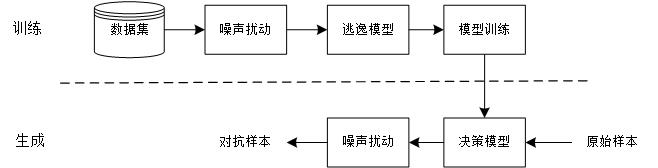
\includegraphics[width=0.75\textwidth]{figures/1.1}
	% \caption[这里的文字将会显示在 listoffigure 中]{这里的文字将会显示在正文中}
	\caption{对抗样本生成基本框架}\label{fig:diagram}
\end{figure}

\begin{enumerate} [label=\arabic*)] 
\item 基于梯度的攻击方法:如FGSM\cite{lupart2023study}(Fast Gradient Sign Method)、BIM\cite{kurakin2016adversarial}(Basic Iterative Method)、PGD\cite{bryniarski2021evading}(Projected Gradient Descent)等,通过利用模型的梯度信息快速生成对抗扰动。这类方法执行效率高,易于实现,广泛用于对抗训练。

Attack Methods Based on Gradient: such as FGSM\cite{lupart2023study} (Fast Gradient Sign Method), BIM\cite{kurakin2016adversarial} (Basic Iterative Method), and PGD\cite{bryniarski2021evading} (Projected Gradient Descent), which generate adversarial disturbance rapidly by utilizing model gradient information. These methods are efficient and easy to implement and are widely used in adversarial sample training.
\item 优化目标驱动方法:如C\&W攻击\cite{carlini2017towards}、DeepFool\cite{moosavi2016deepfool}等,通过构建特定的优化目标函数,最小化扰动幅度同时最大化模型输出的误导性,提高攻击的隐蔽性和精度。

Optimization Objective Driver Methods: such as C\&W attacks\cite{carlini2017towards} and DeepFool\cite{moosavi2016deepfool}, which construct functions optimizing objects to minimize disturbance magnitudes while misleading model maximally, enhancing attack concealment and precision.
\item 迁移型与黑盒攻击方法:此类方法在未知模型结构的情况下依然能实现攻击目标,如使用替代模型生成具有迁移能力的对抗样本,或基于查询机制的无梯度攻击方法,如NES攻击\cite{ilyas2017query}、ZOO攻击\cite{chen2017zoo}等。

Attack Methods Based on Transferability and Black Box: These methods can achieve attack goals without knowing the details of target model’s architecture, such as using transferable adversarial examples generated by alternative models, gradient-free attacks methods based on query mechanisms like NES attacks\cite{ilyas2017query} and ZOO attacks\cite{chen2017zoo}.
\item 对抗样本在安全领域的扩展应用:研究者逐渐将对抗样本技术拓展至文本、音频和恶意代码等复杂数据领域。在恶意软件检测任务中,对抗样本不仅需要误导分类器,更需保持原始代码功能的完整性,这对样本生成算法提出更高要求。

Extensive Applications of Adversarial Examples in Security: Researchers are increasingly extending adversarial example techniques to complex data realms like text, audio, and malicious code. In malware detection tasks, adversarial examples are required to not only mislead classifiers but also preserve the original code’s functional integrity, imposing higher requirements on sample generation algorithms.
\end{enumerate}

Kolosnjaji 等人\cite{kolosnjaji2018adversarial}提出了一种基于梯度的对抗攻击方法,仅修改恶意样本末尾少量字节即可成功绕过以原始字节为输入的深度恶意软件检测模型,且不影响其功能,揭示了此类模型在静态检测场景下的对抗脆弱性。

Kolosnjaji et al.\cite{kolosnjaji2018adversarial} proposed an adversarial attack method based on gradient, which successfully evades malware detection models based on deep learning and taking raw bytes as input by modifying only a few bytes at the end of malicious samples, without influencing their functionality, exposing the limitation of such models in static malware detection scenarios.

Hu和Tan等人在2022年提出了MalGAN\cite{hu2022generating},一种基于生成对抗网络(GAN)的黑盒对抗样本生成方法,用于攻击机器学习恶意软件检测系统。该方法通过训练一个生成器网络,使其生成能够绕过黑盒检测模型的对抗性恶意样本。

Hu and Tan et al. proposed MalGAN\cite{hu2022generating}, a black-box adversarial example generation method based on generating adversarial network (GAN) for attacking malware detection systems based on machine learning in 2022. This method trains a generator network to produce adversarial malware samples that can evade black-box detection models.

Grosse 等人(2017)\cite{grosse2017adversarial}将对抗样本攻击扩展至恶意软件检测领域,提出了一种改进的对抗样本生成方法,可在离散和二值输入空间中生成保持恶意功能的对抗样本。

In 2017, Grosse et al. extended adversarial sample attacks to malware detection realm\cite{grosse2017adversarial}, proposing an advanced adversarial sample generation method that creates adversarial samples that keep malicious functions in discrete and binary input spaces.

Demetrio等人在2019年探讨了卷积神经网络(CNN)在恶意软件检测中的对抗鲁棒性问题\cite{demetrio2019explaining}。研究发现,一些原本在图像分类中有效的攻击方法在恶意软件检测中失效,而 CNN 架构本身也存在特定弱点,可被利用设计新的攻击方式。

Demetrio et al. explored the adversarial robustness of convolutional neural networks (CNNs) in malware detection in 2019\cite{demetrio2019explaining}. Their study found that some origin effective attack methods for image classification failed in malware detection, while the CNN framework itself existed specific weaknesses that can be used to design new attack methods.

近年来,部分研究尝试将强化学习与对抗样本生成结合,建模为一个序列决策过程,使攻击策略更加智能化。

Recently, some studies have attempted to combine Reinforcement Learning and adversarial example generation, modeling it as a sequential decision process that makes attack strategies more intelligent.

Song等人提出了一种基于强化学习的纯黑盒对抗攻击框架\cite{song2022mab},用于生成针对 PE 恶意样本检测器和商业杀毒引擎的对抗样本。该方法将攻击过程建模为多臂老虎机问题,在探索和利用之间寻求最优平衡。Labaca-Castro等人提出AIMED-RL框架\cite{labaca2021aimed},该方法基于分布式双重 DQN,能够在不破坏恶意样本功能的前提下,通过强化学习自动生成对抗样本,实现对恶意软件分类模型的规避。Zhong等人提出了一个基于强化学习的框架\cite{zhong2022reinforcement},用于生成强对抗性的恶意软件样本,以逃避第三方检测器。该方法通过动态规划或时序差分学习自适应地选择最优扰动路径,该路径由Obfusmal、Stealmal和Hollowmal三种扰动方法组合而成。Homayoun等人提出了一种面向硬件恶意软件检测(HMD)系统的多阶段对抗性学习与防御框架\cite{he2024beyond}。该方法针对处理器性能计数器等结构化表格数据,在第一阶段使用有效对抗攻击规避机器学习检测;随后引入基于 Advantage Actor Critic(A2C)的深度强化学习方法实时预测攻击模式,并结合对抗训练增强模型鲁棒性。Li等人\cite{ebrahimi2022adversarial}针对基于机器学习的恶意软件检测器在对抗样本下鲁棒性不足的问题,提出了一种基于对抗最小最大优化的对抗学习框架。该方法将通过强化学习生成的对抗样本引入训练过程,通过攻击策略与检测模型的交替优化提升鲁棒性。

Song et al. proposed a purely black-box adversarial attack framework based on Reinforcement Learning for generating adversarial samples against PE malware detectors and commercial antivirus engines\cite{song2022mab}. This method models the attack process as a multi-armed bandit problem, finding an optimal balance between exploring and utilizing. Labaca-Castro et al. proposed the AIMED-RL framework based on distributed double DQN\cite{labaca2021aimed}, which could automatically generate adversarial samples by using Reinforcement Learning to evade malware classification models. Besides, the functions of malicious samplew are not broken. Zhong et al. raised a framework based on Reinforcement Learning which could be used to generate highly adversarial malware samples to evade third-party malware detectors\cite{zhong2022reinforcement}. This method uses dynamic programming or temporal difference learning to adaptively select optimal disturbance paths that incorporate Obfusmal, Stealmal, and Hollowmal three disturbance methods. Homayoun et al. raised a multi-stage adversarial learning and defense framework targeting hardware malware detection (HMD) systems\cite{he2024beyond}. This method targets structured tabular data, such as processor performance counters. In the first stage, it evades malware detection by using effective adversarial attacks, then introduces a deep Reinforcement Learning approach based on Advantage Actor Critic (A2C) to forecast attack patterns and integrates adversarial training methods to enhance model robustness. Li et al. addressed the issue that malware detectors based on machine learning robustness are insufficient against adversarial examples\cite{ebrahimi2022adversarial}, then offered an adversarial learning framework based on adversarial maximum and minimum optimization. This method integrates adversarial samples generated by Reinforcement Learning into training processes, alternately enhancing robustness by optimizing attack strategies and malware detection models.

尽管已有多种方法取得显著成果,但当前研究仍面临若干挑战。一方面,部分方法过于依赖模型结构或梯度信息,难以适应真实环境中的黑盒场景;另一方面,对抗样本在保证误导性的同时,往往牺牲了样本的可执行性或语义合理性,特别是在代码和文本等高语义数据上。此外,现有研究普遍侧重于攻击单一模型,对于联合防御、多模型集成系统的逃逸效果有限。

Although various methods get significant achievements, current research still faces several challenges. On the one hand, some methods rely excessively on model structure or gradient information, which makes them struggle to adapt to real black-box scenarios. On the other hand, while ensuring misguidance, adversarial examples often reduce sample executability or semantic plausibility, particularly for data that has highly semantic meaning, such as code and text. Furthermore, existing studies generally focus on attacking single models, limiting evasion effects against joint defense or multi-model integrated malware detection systems.

因此,如何在保证样本功能完整与语义一致的前提下,实现对多种检测系统的有效攻击,成为当前研究的重要方向。同时,如何设计通用、轻量、高迁移性的攻击框架,也成为未来研究的关键课题。

Therefore, how to effectively attack multiple detection systems while ensuring sample functional integrity and semantic consistency has become a crucial research direction of current research. Meanwhile, designing universal, light, and highly transferable attack frameworks is also a key challenge for future research.

\section{本文研究内容 Research Content of This Paper}
%\label{sec:features}

本文围绕“基于强化学习的多维度对抗性恶意软件生成方法”展开,旨在突破当前对抗样本生成方法在模型迁移性、扰动精细性及逃逸能力等方面的瓶颈,构建一个具备实用性和泛化性的智能对抗框架。具体研究内容如下:

This study focuses on the "Reinforcement Learning-based multi-dimensional adversarial malware generation method" and aims to overcome the difficulties of adversarial sample generation methods, such as model transferability, disturbance accuracy, and evasion capability by constructing an intelligent adversarial framework with practicality and versatility. The specific research contents are listed as follows:
\begin{enumerate} [label=\arabic*)] 
\item 恶意软件扰动维度建模与设计。针对传统对抗性样本生成方法多以字节插入、节区填充等静态操作为主,缺乏对样本行为层面的深入干预,本文从结构层、指令层与行为层三个维度对原始恶意样本进行扰动建模,系统构建了可控的扰动操作空间。结构层扰动包括节区重命名、节区重排序、空节填充等对样本格式产生改变但不影响可执行性的操作;指令层扰动主要包括无操作指令插入、等价指令替换等轻量级代码层扰动;行为层扰动涉及系统调用替换、配置路径扰动等对动态行为产生微妙变异的操作。这一多维设计旨在提升扰动的多样性与组合能力,为后续的策略学习提供丰富操作选择。

Malware Disturbance Dimension Modeling and Design: To solve the limitation that traditional adversarial sample generation methods mainly rely on static operations that are insufficient for having intervention at the behavioral layer of samples such as byte insertion or section padding, this research models disturbance of original malware from three dimensions—structural layer, instruction layer, and behavioral layer, systematically establishing a controllable disturbance operation space. Structural layer disturbance includes operations that modify sample format without affecting executability, such as section renaming, section resorting, and section padding. Instruction layer disturbance mainly contains slight code level operations like inserting no-operation (NOP) instructions or replacing equivalent instructions. Behavioral layer disturbance is comprised by operations that subtly modify malware dynamic behavior, such as replacing system calls or disturbing configuration paths. This multi-dimensional design aims to enhance disturbance diversity and combining abilities, providing abundant operational choices for following strategy learning.
\item 引入良性样本特征扰动机制。有别于传统使用随机扰动或无效填充字节的方式,本文创新性地引入真实良性软件样本中的特征字节序列作为扰动来源,增强对抗样本的“良性掩盖效应”,提高检测系统误判率。通过构建良性字节库,并对其语义信息进行编码与筛选,在扰动过程中优先选取与目标样本语义接近的良性片段嵌入,使生成样本更具可解释性和混淆性。

Introducing Benign Sample Feature Disturbance Mechanism: Different from traditional methods using random noise or invalid padding bytes, this study innovatively introduces feature byte sequences that are extracted from real benign software samples as disturbance byte sources. This method enhances the "benign concealment effect" of adversarial samples and increases the misjudgment rate of malware detection systems. By constructing a benign byte repository and through encoding and filtering its semantic information, it prioritizes selecting benign fragments similar to the target sample to embed in the target sample during disturbance, which improves the interpretability and obfuscation capability of generated samples.
\item 强化学习环境建模与策略优化方法设计。本文将对抗样本生成过程建模为强化学习中的序列决策问题。状态空间定义为当前恶意样本的扰动历史与静态/动态特征;动作空间为预定义的扰动操作集;奖励函数综合考虑逃逸成功率、扰动成本、执行有效性等多维度指标。为增强序列建模能力,本文引入长短期记忆网络(LSTM)结构,作为策略网络的一部分,建模扰动序列间的时间依赖关系。同时,使用PPO(Proximal Policy Optimization)算法提升策略学习的稳定性和训练效率,缓解强化学习在高维稀疏奖励场景下的训练困难。

Reinforcement Learning Environment Modeling and Strategy Optimization Design: This research regards the adversarial sample generation process as a sequential problem about making decisions in Reinforcement Learning. The state space is defined as the disturbance history, static features, and dynamic features of the current malware sample. The action space is composed of the predefined disturbance operation set. The reward function considers multiple dimensions indicators such as evasion success rate, disturbance cost, and execution effectiveness. To enhance sequential modeling ability, a Long Short-Term Memory (LSTM) network is introduced as a section of the policy network to model the temporal dependencies between perturbation sequences. Besides, the Proximal Policy Optimization (PPO) algorithm is being used to improve the stability and training efficiency of strategy learning, which alleviates the training difficulties in high dimensional sparse reward scenarios.
\item 动态奖励机制设计与泛化能力优化。为提高生成样本的实用性与跨平台攻击能力,本文设计了一个基于目标检测器反馈与扰动代价联合驱动的动态奖励函数,以实现对训练资源和扰动成本的双重约束。		

Dynamic Reward Mechanism Design and Generalization Ability Optimization: To enhance the generated sample practicality and make the generated sample have the ability to attack multiple platforms, this research designs a dynamic reward function driven by target detector feedback and disturbance cost to constrain training resources and disturbance cost.
\end{enumerate}

此外,本文引入多个异构检测器构建多模型训练环境,提升策略泛化能力,使生成的样本不仅能成功绕过训练时的目标模型,还具备较强的迁移性,能够对抗未知或演化型检测系统。

Furthermore, multiple heterogeneous detectors are introduced to construct a multi-model training environment, and enhance strategy generalization, which ensures that generated samples can not only evade the target training model but also have high transferability to confront the detection of unknown or evolving systems.


\section{论文组织结构 Organization Structure of This Thesis}
%\label{sec:requirements}
本论文共分为五章,章节安排如下:

This thesis is comprised of five chapters, organized as follows:

第1章为绪论,主要介绍本研究的背景与动机,分析当前恶意软件检测领域面临的严峻安全形势与技术挑战,明确开展对抗性恶意样本生成研究的必要性。随后概述本研究的目的、意义和技术路线,并梳理国内外在相关领域的研究现状。最后,对论文结构进行总体介绍。

Chapter 1 is an introduction for this thesis, which primarily introduces the background and the motivation of this research, analyzes the severe security condition and technical challenges in the malware detection field, and clarifies the necessity of conducting adversarial malware sample generation research. Therefore, it clarifies the purpose, significance, and technical route of this study, while reviewing the current domestic and international research status in related domains. Finally, it provides an introduction of the thesis’ structure.

第2章为相关技术基础,介绍了研究所涉及的关键理论与技术,包括恶意软件检测技术体系、对抗样本的定义与生成原理、强化学习基础算法(特别是PPO)以及LSTM网络的结构与优势。通过对现有技术的讲解,为后续方法设计和模型构建提供理论支撑。

Chapter 2 presents some related foundational technologies and theories in the research, which includes the malware detection technology system, adversarial examples definitions and generation theories, fundamental Reinforcement Learning algorithms such as PPO, and the structure and advantages of LSTM networks. Through an explanation of existing technologies, it provides theoretical support for subsequent method design and model construction.

第3章为基于强化学习的多维度对抗性样本生成框架设计,主要介绍本文提出的对抗性恶意软件生成架构整体设计。框架包括三个扰动维度:结构扰动、指令扰动与行为扰动,并采用良性样本字节注入机制替代传统的随机扰动方式。此外,描述系统中强化学习环境构建、状态表示、动作定义、奖励机制等核心模块的设计思路,以及智能体PPO+LSTM架构的整体部署逻辑。

Chapter 3 recommends a multi-dimensional adversarial sample generation framework design based on Reinforcement Learning, mainly presenting the overall structure of the adversarial malware generation framework proposed by this research. The framework includes structural perturbations, instruction perturbations, and behavioral perturbations three disturbance dimensions. Besides, it replaces traditional random disturbance methods with a novel benign sample byte injection mechanism. Additionally, it describes the core modules design logic, including constructing the Reinforcement Learning environment, representing states, defining actions, designing reward mechanisms, and the PPO+LSTM agent architecture overall deployment.

第4章为关键模块实现与方法细化,将对前章所提出的框架设计进行具体实现层面的详细展开,主要包括多维扰动策略生成过程、扰动数据集构建方法、良性字节选择机制、扰动语义保持策略、PPO+LSTM智能体训练流程等内容。通过模块化描述,清晰呈现模型训练与对抗样本生成的全过程。

Chapter 4 discusses implementing key modules and refining methods and provides concrete implementation details for the framework proposed in the previous chapter, which includes the multi-dimensional disturbance strategy generation process, dataset construction methods for disturbance, benign byte selection mechanisms, semantic strategies preservation during disturbance, and the PPO+LSTM agent training workflow. Through the modular descriptions, it can clearly express the entire process of model training and adversarial sample generation.

第5章为实验评估与结果分析,本章设计并执行了一系列实验以验证所提方法的有效性与实用性。通过在多个主流恶意软件检测模型(如基于静态分析和动态行为的检测系统)上进行对抗测试,评估生成样本的逃逸率、扰动成本、泛化能力及其对抗演化检测模型的鲁棒性。同时,与传统扰动方法及无序强化学习方法进行对比,展现本方法的优势与研究价值。

Chapter 5 evaluates the experiment and analyzes the results. This chapter designs and conducts a series of experiments to verify the effectiveness and practicality of the proposed method. Through testing multiple prevalent malware detection models based on static analysis and dynamic behavior analysis, it evaluates the evasion rate, disturbance cost, generalization capability, and robustness of generated adversarial samples against evolving detection models. By comparing analyses based on traditional perturbation methods or non-sequential Reinforcement Learning approaches, the method proposed in this research demonstrates its advantages and research value.


%%
% The BIThesis Template for Graduate Thesis
%
% Copyright 2020-2023 Yang Yating, BITNP
%
% This work may be distributed and/or modified under the
% conditions of the LaTeX Project Public License, either version 1.3
% of this license or (at your option) any later version.
% The latest version of this license is in
%   https://www.latex-project.org/lppl.txt
% and version 1.3 or later is part of all distributions of LaTeX
% version 2005/12/01 or later.
%
% This work has the LPPL maintenance status `maintained'.
%
% The Current Maintainer of this work is Feng Kaiyu.
%
% Compile with: xelatex -> biber -> xelatex -> xelatex

\chapter{相关技术与工作 Some Related Foundational Technologies and Work}
\section{ELF文件结构 ELF File Structure}
ELF(Executable and Linkable Format)文件格式是目前类 Unix 操作系统(如 Linux、FreeBSD)中广泛采用的一种标准二进制格式,用于描述可执行文件、目标文件、共享库和内核转储文件。由于其良好的可扩展性与跨平台支持,ELF 格式被认为是现代操作系统中程序执行与链接的核心桥梁。一个典型的 ELF 文件主要包括以下四个关键结构:

The ELF file format, the abbreviation for Executable and Linkable Format, is a standard binary format that is widely adopted in Unix-like operating systems such as Linux and FreeBSD for describing executable files, object files, shared libraries, and kernel dump files. Because of its superior extensibility and support among different platforms, the ELF format is defined as a core bridge for executing programs and linking libraries in modern operating systems. A typical ELF file primarily contains the following four critical structures:
\begin{enumerate} [label=\arabic*)] 
\item ELF 头(ELF Header)

ELF 文件的开头是一个固定大小的 ELF 头部,用于描述整个文件的总体信息。它包含了魔数(magic number)用于识别 ELF 文件、目标机器架构(如 x86、ARM)、文件类型(可执行文件、共享对象或目标文件)、程序入口地址、程序头表偏移、节头表偏移、各个表的数量与大小等。操作系统的加载器首先读取这一部分信息来判断该文件是否为合法的 ELF 文件,并根据提供的偏移值进一步解析程序头和节头信息。

ELF Header:
The beginning of an ELF file contains a definite size ELF header that describes the file‘s information which includes the magic number for identifying ELF files, the target machine architecture such as x86 or ARM, the file type such as executable files or shared objects, the program entry point address, program header table offset, section header table offset, and respective tables’ number and size. When it is executed, the operation system loader first reads this section to determine whether the file is a valid ELF file or the file is only an invalid file whose file extension was changed and then analyzes the program header and section header information using the provided offsets.


\item 程序头表(Program Header Table)

程序头表是面向操作系统加载器的结构,主要描述程序运行时需要载入内存的“段”(Segment)。每一项描述了一个段的类型、在文件中的偏移、在内存中的虚拟地址、所需的权限(可读、可写、可执行)以及其大小等信息。例如,常见的代码段 .text、数据段 .data 等,都会在程序头表中有对应的段描述。加载器正是依据程序头表将相应部分映射至进程的地址空间中。

The program header table is a structure targeting operation system loaders, primarily describing segments that are required to be loaded into memory when the program is executed. Each item of the program header table describes a segment's type, file offset, virtual address in memory, required permissions (readable, writable, executable), and size. For example, common code segments like .text and data segments like .data have relevant segment descriptions in the program header table. According to this table, the loader maps relevant sections into the address space of the executing process.

\item 节(Section)

节是编译和链接阶段使用的逻辑组织单元,用于存储源代码生成的不同类型的数据,如 .text(代码段)、.data(已初始化的数据段)、.bss(未初始化的数据段)、.rodata(只读数据)、.symtab(符号表)、.strtab(字符串表)、.debug(调试信息)等。节通常不会被直接加载进内存执行,而是由链接器使用,或被分析工具读取以进行二进制分析、反汇编和静态分析等任务。

Sections are logical organization units that store different kinds of data generated from source code. They are used for compilation and linking phases. Section examples include .text (storage code), .data (storage initialized data), .bss (storage uninitialized data), .rodata (storage read-only data), .symtab (symbol table), .strtab (string table), and .debug (debug information). Sections are commonly not loaded directly into memory for execution but are used by linkers or read by analysis tools for operations like binary analysis, disassembly, and static analysis.

\item 节头表(Section Header Table)

节头表则是面向链接器和调试器的结构,它记录了每个节的元信息,如名称、类型、权限、文件偏移、地址、大小等。每一项对应一个节,操作系统或工具链通过节头表来快速定位和解析各节内容。在某些可执行文件中,节头表甚至可以被省略,以减小文件体积或增加反分析难度,但这不会影响程序的加载运行,因为程序的执行依赖的是程序头表,而非节信息。

The section header table is a structure facing linkers and debuggers. It records metadata for each section, including its name, type, permissions, file offset, address, and size. Each item corresponds to a section. Operating systems and tool chains use the section header table to quickly locate and parse section contents. In some executable files, the section header table can be omitted to reduce file size or to increase disassembly difficulty. However, it does not affect program loading and executing because program execution relies on the program header table rather than section information.  

\end{enumerate}

\begin{figure}[hbt]
	\centering
	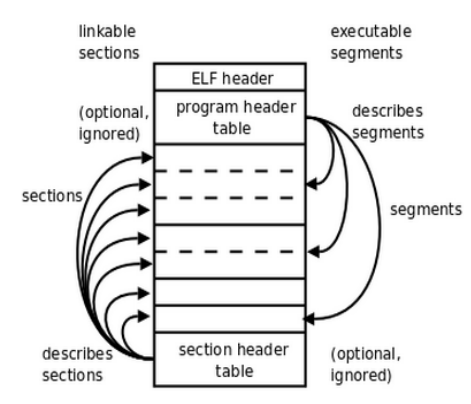
\includegraphics[width=0.75\textwidth]{figures/2.1}
	% \caption[这里的文字将会显示在 listoffigure 中]{这里的文字将会显示在正文中}
	\caption{ELF文件结构 ELF File Structure}\label{fig:2.1}
\end{figure}

\section{恶意软件检测技术 Malware Detection Technologies}

随着信息技术的快速发展和应用系统的日益复杂,恶意软件在网络空间中的传播形式不断演化,攻击手段愈加隐蔽与智能化,传统的防护机制正面临严峻挑战。据全球网络安全厂商统计,2023年全球每天新增恶意软件样本超过50万个,其中近30\%的样本采用了变种、加壳、动态加载等手段以逃避检测,呈现出高度自动化和持续化的攻击特征。这些趋势表明,恶意软件检测正成为保障网络空间安全的关键技术环节。
目前,恶意软件检测技术主要分为以下三类,如图\ref{fig:2.2}所示:
With technology's rapid development and application systems' complexity enhancement, malware propagation forms in cyberspace continue to evolve, while attack techniques become more covert and intelligent. Traditional defense mechanisms face severe challenges. According to global cybersecurity companies, over 500,000 new malware samples emerged daily from all over the world in 2023, with nearly 30\% of them adopting methods such as mutation, packing, and dynamic loading to evade detection, demonstrating highly automated and consistent attack characteristics. These trends suggest that malware detection has become a critical technical link for ensuring cyberspace security.
Currently, malware detection technologies are primarily classified into the following three types, which are expressed in Figure \ref{fig:2.2}:

\begin{figure}[hbt]
	\centering
	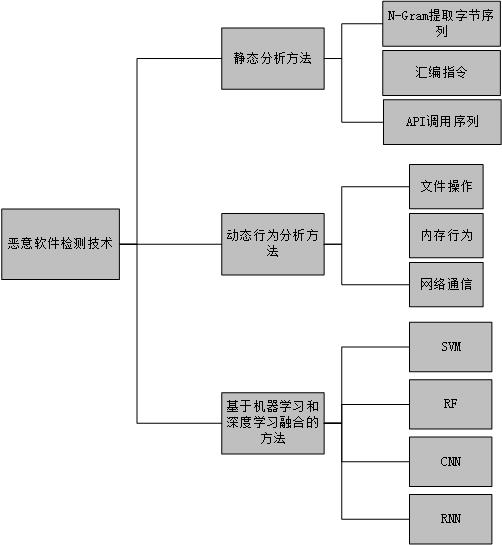
\includegraphics[width=0.75\textwidth]{figures/2.2}
	% \caption[这里的文字将会显示在 listoffigure 中]{这里的文字将会显示在正文中}
	\caption{恶意软件检测方法分类 Malware Detection Methods Classification}\label{fig:2.2}
\end{figure}

%\begin{enumerate} [label=(\arabic*)] 
 
(1)静态分析方法  Static Analysis Methods

静态分析是最早应用于恶意代码检测的技术手段,主要通过对软件的二进制文件进行逆向工程分析,从中提取诸如特征码、字符串信息、导入表、节区结构、指令序列、操作码频率等静态特征,再使用签名匹配或机器学习方法进行分类判断。Kumar等\cite{kumar2019learning}通过组合PE头的原始值与派生值,并比较集成特征集与原始特征集,证明了基于前者的分类器能以较高准确度和较低成本检测和分类恶意软件。Yan等\cite{yan2019classifying}提出了一种利用深度图卷积神经网络对控制流图(CFG)进行嵌入的新型恶意软件分类系统,并在两个包含超过20,000个样本的大型数据集上验证了该系统的有效性。Corlatescu等\cite{corlatescu2023embersim}提出了基于静态分析的恶意软件检测框架,利用文件结构信息和元数据构建了EMBER基准数据集。Ling等\cite{ling2022malgraph}提出MalGraph,一种基于层次图神经网络的方法,用于鲁棒的Windows恶意软件检测,通过函数调用图和控制流图捕捉可执行文件的交互与结构语义。

Static analysis is the earliest technique used for malicious code detection, which mainly first uses reverse engineering of software binary files to extract static features such as traits, string information, import tables, section structures, instruction sequences, and operation code frequencies, then uses signature matching or machine learning methods to classify and judge. Kumar et al. proved that classifiers based on combining raw and derived values of PE headers and comparing integrated feature sets against original feature sets can detect and classify malware with high accuracy\cite{kumar2019learning}. Yan et al. proposed a novel malware classification system using deep graph convolutional networks to embed control flow graphs (CFGs), validating its effectiveness on two large datasets that contain over 20,000 samples\cite{yan2019classifying}. Corlatescu et al. issued a static analysis-based malware detection framework and constructed the EMBER benchmark dataset based on file structure information and metadata\cite{corlatescu2023embersim}. Ling et al. raised MalGraph, a neural network method relying on hierarchical graph for robust Windows malware detection, capturing executable file interaction and structure semantics through function call graphs and control flow graphs\cite{ling2022malgraph}.

该方法优点是速度快、资源消耗低,适合大规模样本初筛。但它的缺点也很明显:对经过加壳、混淆、代码插入等技术处理的恶意软件识别能力较弱,容易被绕过。

This approach's advantages include high speed and low resource consumption, making it suitable for large-scale sample initial sifting. However, its weaknesses are also obvious, such as lacking the ability to recognize malware processed with packing, obfuscation, and code injection, which can make malware evade easily.

(2)动态行为分析方法

动态分析通过在虚拟沙箱或受控环境中执行可疑程序,监控其运行时的行为,包括系统调用序列、文件操作、注册表修改、网络通信等动态特征,以此判断程序的恶意性。Trizna等\cite{trizna2024nebula}提出了一种名为Nebula的自注意力Transformer架构,用于动态恶意软件分析。通过对行为报告进行标记化、过滤、归一化和编码,适配Transformer架构,并进行全面消融研究,评估系统组件对性能的影响。Bhat等\cite{bhat2023system}利用系统调用分析对Android应用进行动态行为分析,提取动态特征后,使用集成学习算法分类。Li等\cite{li2022novel}在安全虚拟环境中对软件API调用序列进行动态分析,并将这些序列转化为多种特征表示,使用深度学习模型(包括Bi-LSTM)进行分类。Chen等\cite{chen2022cruparamer}提出了基于参数增强的API序列学习方法,通过深度神经网络训练,具有较高的检测鲁棒性和泛化能力。Rohini等\cite{rohini2024magic}提出MAGIC方法,通过行为共现和回归分析量化恶意软件行为,实验结果显示MAGIC比传统方法更准确地反映签名的恶意程度,提高了恶意软件威胁的防御能力。

Dynamic analysis executes suspicious programs in virtual sandboxes or controlled environments, monitoring their behaviors which include dynamic features such as system call sequences, file operations, registry modifications, and network communications when they are executed to determine whether the programs are malicious. Trizna et al. proposed Nebula, a self-attention Transformer architecture for dynamic malware analysis\cite{trizna2024nebula}. Through noting, filtering, normalizing, and encoding behavioral reports and adapting Transformer structure, they conducted comprehensive studies to evaluate system component effect on performance. Bhat et al. performed dynamic behavioral analysis on Android applications by system call analyzing, extracting dynamic features to use integrated learning algorithms for classification\cite{bhat2023system}. Li et al. dynamically analyzed software API call sequences in secure virtual environments, transformed these sequences into multiple feature expressions, and using deep learning models including Bi-LSTM to classify them\cite{li2022novel}. Chen et al. proposed an API sequence learning method based on parameter augmentation, which can achieve high detection robustness and generalization ability through deep neural network training\cite{chen2022cruparamer}. Rohini et al. raised MAGIC, which quantifies malware behaviors through behavioral co-occurrence and regression analysis\cite{rohini2024magic}. Experimental results showed MAGIC is more accurate in reflecting signature maliciousness than traditional methods, enhancing malware defense capabilities.

这种方法更侧重于检测实际行为,因此在应对变种或混淆样本方面具有更好的鲁棒性。然而,其缺点在于分析开销较大,容易被延时执行或沙箱检测绕过。此外,一些高度针对性的APT攻击样本在沙箱中可能不会暴露其真实行为,从而导致漏报。

This method focuses more on detecting actual behaviors, which means it is robust against mutation or obfuscated samples. However, it suffers from higher resource consumption and remains vulnerable to being evaded through delayed execution or anti sandbox detection techniques. Furthermore, some highly targeted APT attack samples may not reveal true behaviors in virtual sandboxes, which leads to false negatives.

(3)基于机器学习和深度学习融合的方法 Methods Based on Combing Machine Learning and Deep Learning

近年来,随着人工智能技术的快速发展,越来越多的研究者将机器学习与深度学习方法应用于恶意软件检测任务。通过从样本中提取静态或动态特征,再使用如支持向量机(SVM)、随机森林(RF)、卷积神经网络(CNN)、循环神经网络(RNN)等模型进行分类训练,已在多个公开数据集上取得了较好的检测效果。Ngo等\cite{ngo2023fast}提出了一种结合静态和动态特征的快速恶意软件检测方法,利用迁移学习提升检测效率。通过深度学习提取潜在特征表示,解决特征维度不一致的问题,并使用知识蒸馏技术将聚合特征的知识迁移到静态特征模型中,实现快速检测。Shar等\cite{shar2023experimental}从Android应用中提取14种特征,比较传统机器学习(如随机森林)和深度学习(如循环神经网络)在这些特征上的表现。Bashir等\cite{bashir2024hybrid}提取Android应用的静态和动态特征(如API调用和权限),并使用SVM、K-NN、NB及集成学习方法分类。

Recently, with the rapid development of artificial intelligence, an increasing number of researchers adopt machine learning and deep learning methods to solve malware detection tasks. By extracting static or dynamic features from samples and training classification models such as Support Vector Machines (SVM), Random Forest (RF), Convolutional Neural Networks (CNN), and Recurrent Neural Networks (RNN), researchers achieved significant detection results on multiple public datasets. Ngo et al. introduced a rapid malware detection method combining static and dynamic features, enhancing detection efficiency via transfer learning\cite{ngo2023fast}. Through deep learning extracting latent characteristics to resolve feature dimension inconsistency problems and knowledge distillation, this method transfers aggregated feature knowledge to static feature models, which can achieve detect more rapidly. Shar et al. extracted 14 features from Android applications, comparing traditional machine learning methods such as random forest and deep learning methods such as recurrent neural networks performance on these features\cite{shar2023experimental}. Bashir et al. extracted static and dynamic features, such as API calls and permission, from Android applications, and classified them by using SVM, K-NN, Naive Bayes, and integrated learning methods\cite{bashir2024hybrid}.

恶意软件检测技术正从传统的签名匹配逐渐迈向智能化、自适应的发展方向。Bensaoud和Kalita\cite{bensaoud2022deep}通过生成恶意软件的位图和PNG图像并输入深度学习模型进行分类,采用硬参数共享和软参数共享策略,成功检测使用各种混淆技术的恶意软件。Conti等\cite{conti2022few}提出了一种基于GEM图像的深度学习方法,结合灰度矩阵图像、GLCM纹理特征、马尔可夫图像和熵图像,用于较浅的CNN架构,提升了训练和分类效率。Mallik等\cite{mallik2022conrec}通过将恶意软件样本转为灰度图像,并利用卷积神经网络捕捉结构相似性,结合BiLSTM层和VGG16层的输出,进行恶意软件家族分类,表现出色。

尽管检测方法不断优化,但随着攻击者技术手段的日益多样化,现有检测系统仍难以全面覆盖所有威胁类型,尤其是对抗性样本的出现,进一步揭示了现有模型的脆弱性。因此,如何在保证检测准确率的同时,提升模型对抗攻击的鲁棒性,成为当前恶意软件检测领域的重要研究方向之一。

该方法具有一定的自适应能力和特征抽象能力,但其检测结果往往依赖于训练数据的分布一致性,面对对抗样本或新型威胁时仍存在鲁棒性不足的问题。
%\end{enumerate}

\section{对抗性恶意软件}
近年来,随着深度学习技术在恶意软件检测中的广泛应用,基于神经网络的分类模型成为主流检测手段之一。然而,大量研究发现,深度神经网络虽然在标准测试样本上表现出色,却容易受到“对抗样本(Adversarial Examples)”的干扰。攻击者通过对输入数据添加轻微但精心设计的扰动,能够误导模型做出错误判断。这种攻击方式在图像识别、语音识别等领域已有广泛研究,并逐步扩展到网络安全领域,尤其是恶意软件检测。

所谓对抗性恶意软件(Adversarial Malware),是指攻击者在不破坏原有恶意功能的前提下,对恶意样本进行精细化扰动,使其在被检测时被误识为正常程序,从而绕过检测系统。这些扰动可以在代码层面(如指令插入、控制流调整)、结构层面(如节表改写、符号表扰动),或行为层面(如API调用序列伪装)实施,具有高度隐蔽性和针对性。


与图像等静态数据不同,恶意软件样本具有复杂的执行语义和潜在行为逻辑,因此对抗性样本的生成不仅要保证样本在结构上的有效性,更要保持其原始攻击行为的可执行性。这一特点使得恶意软件领域的对抗样本生成问题更加复杂与挑战性更高。


目前已有多种方法被提出用于生成对抗性恶意软件,主要包括以下几类:


基于梯度的扰动方法:如FGSM\cite{lupart2023study}(Fast Gradient Sign Method)、PGD\cite{bryniarski2021evading}(Projected Gradient Descent)等方法,将样本视为向量,通过计算模型梯度找到最易引发误判的方向添加扰动。但此类方法大多适用于图像等连续空间,对可执行文件中的离散结构处理效果有限。


启发式与搜索方法:这类方法将扰动操作建模为搜索问题,利用遗传算法\cite{wang2022black}、模拟退火\cite{bertsimas1993simulated}、蒙特卡洛树搜索\cite{chaslot2010monte}等手段,在可执行性约束下寻找最佳扰动路径。其优点是可定制性强,但搜索效率与样本质量之间常常存在权衡。

基于强化学习的方法:近年来,强化学习(RL)因其在策略学习方面的优势,逐渐成为对抗样本生成研究的热点。攻击者构建一个智能体,以规避检测系统为奖励目标,学习一系列扰动策略。常见方法如基于Q-learning\cite{watkins1992q}、DQN\cite{osband2016deep}、PPO\cite{yu2022surprising}(Proximal Policy Optimization)等。这类方法能在保证样本合法性的前提下,实现自适应扰动策略的学习与优化。

对抗性恶意软件的研究不仅揭示了现有检测系统的潜在脆弱性,也推动了鲁棒性检测模型和对抗训练机制的快速发展。然而,如何在扰动成本、逃逸能力和语义一致性之间取得平衡,仍是该领域面临的核心挑战之一。尤其是在对抗样本跨模型迁移性、抗演化检测能力方面,仍需深入研究。

\section{强化学习}

强化学习(Reinforcement Learning, RL)是一种基于试错机制(trial and error)进行学习的人工智能方法,其核心思想是智能体(Agent)通过与环(Environment)的交互,在获得奖励信号的基础上不断调整策略,以最大化长期收益。与监督学习不同,强化学习并不依赖于明确的标签信息,而是通过环境反馈学习行为的价值,具有较强的自适应性与在线学习能力,因而广泛应用于博弈策略优化、机器人控制、自然语言处理及对抗样本生成等任务中。

强化学习过程通常可以使用马尔可夫决策过程(Markov Decision Process, MDP)建模,MDP由一个五元组(S, A, P, R, γ)构成,其中表示所有可能的环境状态的集合。每一个状态刻画了当前环境的完整信息,它是Agent进行决策时观察到的依据。表示所有可能的动作或行为的集合。Agent在某一特定状态下可以选择一个动作  来与环境进行交互。 定义了环境的动态变化规律,即在状态下采取动作后转移到下一个状态的概率,通常表示为:这一性质体现了马尔可夫性,即下一个状态只与当前状态和当前动作有关,与过去的历史无关。 是即时奖励函数,表示在状态  下采取动作后,环境给予Agent的即时反馈,记为 。奖励信号用于指导Agent的学习过程,使其调整行为以获取更多的累计奖励。 是一个折扣因子,用于平衡短期奖励与长期奖励的重要性。较小的  倾向于让Agent更关注近期的奖励,而较大的则鼓励Agent考虑长期累积收益。

\begin{figure}[hbt]
	\centering
	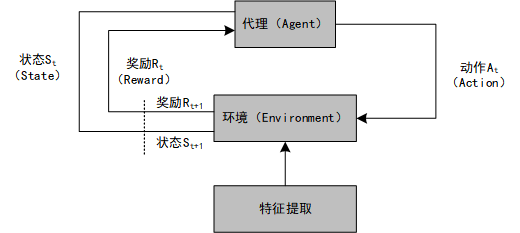
\includegraphics[width=0.75\textwidth]{figures/2.3}
	% \caption[这里的文字将会显示在 listoffigure 中]{这里的文字将会显示在正文中}
	\caption{马尔可夫决策过程}\label{fig:2.3}
\end{figure}

在实际的强化学习交互过程中,智能体(Agent)遵循以下步骤循环进行:
\begin{enumerate} [label=\arabic*)] 
	
\item 观察状态:在时间步 ,Agent观察到当前的环境状态 。
\item 选择动作:基于当前策略 ,Agent选择一个动作 。
\item 执行动作并反馈:动作  作用于环境,环境根据转移概率  跳转到下一个状态 ,并反馈一个即时奖励 。
\item 更新策略(学习):Agent利用所得到的状态、动作、奖励以及新的状态信息更新其内部策略,以期在未来做出更优的决策。

\end{enumerate}

强化学习的目标是学习一个最优策略 ,使得在任意状态下采取的动作能够最大化未来的累计奖励。累计奖励定义为从当前时刻  开始,未来各时刻奖励的折扣和:
\begin{equation}
	\label{eq:reward}
	\boldsymbol{G}_t = \sum_{k=0}^{\infty} \gamma^k r_{t+k}
\end{equation}

其中,\( r_{t+k} \) 表示从时刻 \( t \) 开始第 \( k \) 步时获得的奖励;\( \gamma^k \) 表示第 \( k \) 步奖励的折扣因子。

在强化学习中,策略(Policy)是指导智能体在不同状态下选择动作的规则。策略可以是确定性的,也可以是随机性的。策略优化是强化学习的核心目标之一,常见的方法包括直接优化策略的梯度方法,如策略梯度(Policy Gradient)算法\cite{silver2014deterministic},以及近些年提出的PPO\cite{yu2022surprising}(Proximal Policy Optimization)、TRPO\cite{schulman2015trust}(Trust Region Policy Optimization)等更稳定、高效的优化方法。策略优化关注的是如何基于交互经验调整智能体的行为,以更好地达成目标。

除了直接优化策略之外,强化学习中还广泛使用价值函数(Value Function)来间接指导策略改进。价值函数评估智能体在特定状态或状态-动作对上能够获得的期望累计奖励,通常包括状态价值函数V(s)和动作价值函数Q(s,a)。通过对价值函数的学习,智能体能够更有针对性地选择动作。价值函数的估计可以通过动态规划(如价值迭代、策略迭代)、蒙特卡洛方法\cite{chaslot2010monte}(Monte Carlo Methods)、或时间差分学习\cite{tesauro1991practical}(Temporal Difference Learning)等技术来实现。

强化学习过程中,智能体面临探索(Exploration)与利用(Exploitation)的权衡问题。探索意味着尝试新的、未验证过的动作,以期发现更优的决策路径;而利用则是依据已有知识选择当前认为最优的动作以获取最大回报。如何在探索和利用之间达到合理平衡,直接影响学习效率和最终性能。常见的探索机制包括ε-贪婪策略\cite{wunder2010classes}(Epsilon-Greedy)、基于置信上界\cite{auer2002finite}(Upper Confidence Bound, UCB)的方法、以及基于策略熵的鼓励机制(Entropy Regularization)。

强化学习方法可以根据是否需要建模环境动态而划分为基于模型(Model-Based)和无模型(Model-Free)两大类。基于模型的方法试图学习环境的状态转移规律和奖励机制,从而通过模拟来提高学习效率,如Dyna-Q\cite{peng2018deep}算法。相比之下,无模型的方法则直接根据交互数据学习策略或价值函数,无需显式推断环境模型,代表算法包括深度Q网络(DQN)、策略梯度方法等。基于模型的方法在样本效率上具有潜在优势,但通常面临模型误差带来的累积偏差问题。

近年来,深度强化学习\cite{li2019deep}(Deep Reinforcement Learning, DRL)技术的兴起,使得强化学习能够处理高维、复杂的输入空间。通过引入深度神经网络作为策略函数或价值函数的近似器,DRL极大地拓展了强化学习的应用边界。例如,DQN使用卷积神经网络处理原始像素输入,成功在Atari游戏中达到人类水平;而DDPG、A3C、PPO等方法则将深度学习与连续控制任务结合,在机器人控制、自动驾驶等领域表现出色。深度强化学习的挑战主要在于训练不稳定性和样本效率问题,因此在研究中引入了经验回放、目标网络、归一化技术等一系列改进措施。

此外,面对复杂任务和长时间尺度的决策需求,强化学习也发展出层次化学习(Hierarchical Reinforcement Learning, HRL)\cite{nachum2018data}的方法。通过引入子任务(Options)或多层次的策略结构,HRL能够在抽象层次上分解决策问题,提升学习效率和泛化能力。层次强化学习方法如FeUdal Networks、Options Framework在多阶段任务规划中展现了明显优势。

在多智能体环境中,强化学习技术进一步拓展到多智能体强化学习(Multi-Agent Reinforcement Learning, MARL)领域。MARL研究多个智能体在同一环境中相互作用、竞争或协作的学习过程。针对多智能体系统中策略非平稳性的问题,提出了集中式训练与分布式执行(CTDE)框架、对抗性自博弈(Self-Play)等方法,广泛应用于博弈决策、群体智能、对抗训练等方向。

总体来看,强化学习技术体系涵盖了从基础建模到复杂策略优化、从单智能体学习到多智能体协作的广泛内容。随着计算能力提升和算法不断创新,强化学习正在成为解决复杂智能决策问题不可或缺的重要技术。

\section{神经网络与时序建模技术}

神经网络(Neural Networks)是一类模拟人脑神经元结构与运行机制的计算模型,广泛应用于图像识别、自然语言处理、智能决策等领域。其基本结构包括输入层、一个或多个隐藏层和输出层。每一层通过权重连接前一层神经元,并使用激活函数引入非线性能力,使网络能够逼近任意复杂的非线性映射关系。

神经网络的核心优势在于其强大的表示能力,尤其在数据量充足的情况下,能够自动学习数据中的高阶抽象特征,替代传统人工设计特征的方式,大幅提升模型的泛化性能与适应能力。

在安全领域,神经网络已被用于恶意软件检测、异常行为识别、攻击流量检测等任务,并取得显著成果。然而,由于很多安全任务具有时间依赖性强、上下文联系紧密、行为逻辑复杂等特点,传统的前馈神经网络往往无法有效捕捉这些动态特征。

\subsection{循环神经网络(RNN)}

循环神经网络(Recurrent Neural Network,RNN)是一种专门用于处理序列数据的神经网络模型,其核心特点是具有“记忆能力”,即在处理当前输入时能够利用以往时间步的信息。与传统前馈神经网络不同,RNN的隐藏层神经元不仅接收当前时刻的输入,还接收上一个时刻隐藏层的输出,从而实现了对时间序列的依赖建模。这种结构使RNN特别适合处理语言文本、语音、视频帧序列等具有时间顺序的数据。

在RNN中,每一个时间步的计算会将上一个时间步的状态(隐藏层的输出)传递到下一个时间步,并结合当前输入进行处理,实现序列中信息的传递和积累。但在实际训练过程中,由于反向传播时梯度要经过多个时间步回传,RNN容易出现“梯度消失”或“梯度爆炸”的问题,导致模型在长序列中难以捕捉长期依赖关系。

\begin{figure}[hbt]
	\centering
	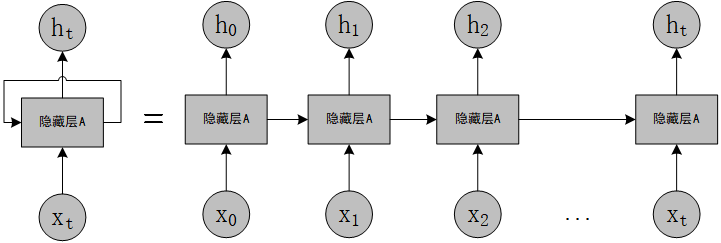
\includegraphics[width=0.75\textwidth]{figures/2.4}
	% \caption[这里的文字将会显示在 listoffigure 中]{这里的文字将会显示在正文中}
	\caption{RNN神经网络结构}\label{fig:2.4}
\end{figure}

为了解决这一问题,研究者提出了多种改进结构,其中最具代表性的是长短期记
忆网络(Long Short-Term Memory, LSTM)和门控循环单元(Gated Recurrent Unit, GRU)。这些改进模型通过引入门控机制(如输入门、遗忘门、输出门)来控制信息
的流入、保留和输出,有效缓解了传统 RNN 在长序列建模中的不足。

RNN及其变种在诸多序列建模任务中展现出强大的性能,特别是在自然语言处
理、机器翻译、语音识别、恶意行为序列建模等领域中,为强化学习、时序建模和序
列生成等应用提供了坚实的基础。

\subsection{长短期记忆网络(LSTM)}

长短期记忆网络(Long Short-Term Memory,LSTM)\cite{graves2012long}是一种特殊的循环神经网络(RNN)结构,旨在解决传统RNN在处理长序列数据时面临的“梯度消失”和“梯度爆炸”问题。与传统RNN相比,LSTM通过引入精心设计的“门控机制”,能够在序列中选择性地记住或忘记信息,从而有效捕捉长期依赖关系,广泛应用于自然语言处理、语音识别、时间序列预测等任务。

LSTM的核心结构包含三个门控单元:输入门(Input Gate)、遗忘门(Forget Gate)和输出门(Output Gate),以及一个单元状态(Cell State),用于携带长期记忆信息。

输入门:控制当前输入信息中哪些部分可以被写入到记忆单元中;

遗忘门:决定前一时刻的记忆状态中哪些信息应该被保留、哪些应该被遗忘;

输出门:则决定当前时刻的记忆状态中哪些内容将作为隐藏状态传递到下一时刻。

LSTM的关键是通过这三个门的配合,实现对信息流的精确控制,从而保留对模型预测有用的信息,丢弃无用或冗余的信息。其信息流如下:首先,遗忘门根据当前输入和前一时刻的隐藏状态,决定哪些旧信息要被“遗忘”;接着,输入门决定要将多少当前输入的新信息写入记忆单元;然后,更新记忆状态;最后,输出门根据当前记忆状态输出一个隐藏状态,用于传递到下一个时间步。
LSTM的这种设计使得它可以在长序列中持续保留有效信息,并忽略无关部分,克服了传统RNN在长距离依赖建模方面的劣势。

\begin{figure}[hbt]
	\centering
	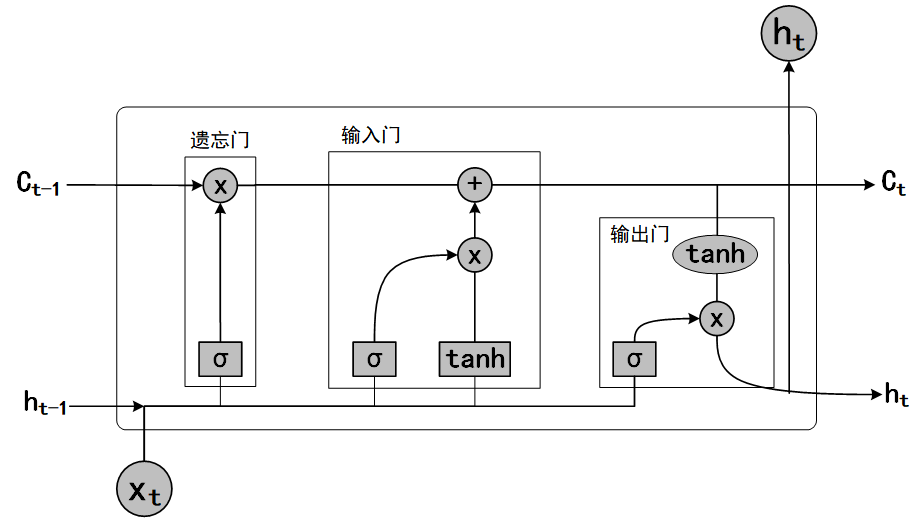
\includegraphics[width=0.75\textwidth]{figures/2.5}
	% \caption[这里的文字将会显示在 listoffigure 中]{这里的文字将会显示在正文中}
	\caption{LSTM基本数据单元结构}\label{fig:2.5}
\end{figure}

由于恶意软件的行为特征和扰动操作本质上具有明显的时序依赖性和上下文联系。恶意样本在执行过程中会形成一系列调用序列、系统行为或指令流,这些序列中的上下文信息对判断恶意行为及实施有效扰动具有重要价值。传统的全连接神经网络或标准循环神经网络(RNN)在处理这类时序数据时,往往难以保持长期依赖,容易遗忘序列中早期的关键信息。而 LSTM 网络通过引入门控机制(包括输入门、遗忘门和输出门),能够有效控制信息的记忆与遗忘,从而保留长期依赖关系,提升模型对扰动序列语义结构的建模能力。具体而言,在生成扰动策略时,LSTM 能够根据当前样本结构状态和历史扰动操作,动态调整策略输出,从而生成更具“攻击性”同时又具备高隐蔽性的对抗扰动。这种记忆能力对于生成具有“顺序逻辑”且能逃避检测系统的恶意行为非常关键。

\section{PPO}

Proximal Policy Optimization(PPO)\cite{yu2022surprising}是一种基于策略梯度的强化学习算法,由 OpenAI 于 2017 年提出。作为 Trust Region Policy Optimization(TRPO)的改进版本,PPO 保留了 TRPO 中稳定更新策略的核心思想,同时大幅简化了算法的实现和训练流程。由于其良好的稳定性与效率,PPO 已成为深度强化学习领域中应用最广泛、表现最为稳定的算法之一。

PPO 的核心思想在于限制新旧策略之间的变化幅度,从而避免策略在更新过程中发生剧烈波动,保证学习过程的稳定性。与传统策略梯度方法直接最大化目标不同,PPO 引入了裁剪目标函数(clipped objective)或基于 KL 散度的惩罚项,用以约束新旧策略的差异。

在裁剪目标函数形式下,PPO 的优化目标为:
\begin{equation}
	\boldsymbol{r}_t(\theta) = \frac{\boldsymbol{\pi}_\theta(\boldsymbol{a}_t | \boldsymbol{s}_t)}{\boldsymbol{\pi}_{\theta_{\text{old}}}(\boldsymbol{a}_t | \boldsymbol{s}_t)}
\end{equation}

其中,\( \boldsymbol{r}_t(\theta) \) 表示当前策略与旧策略在动作概率上的比值。通过最小化裁剪后的目标函数,可以有效防止策略更新偏离旧策略过远,从而提升训练过程的稳定性。

PPO具有诸多显著优势。其稳定性强,通过引入“剪切”目标函数限制每一步策略更新的幅度,从而有效避免了策略在训练过程中发生剧烈变化或崩溃的问题,提升了训练的可靠性。其次,PPO易于实现,相较于 TRPO(Trust Region Policy Optimization)等算法,不需要进行二阶导数计算或求解复杂的约束优化问题,因此更易于在工程中部署和调试,拥有更好的实用性。此外,PPO 还展现出良好的泛化能力,适用于多种不同类型的任务和环境,尤其在处理高维状态空间、复杂交互场景(如机器人控制、游戏智能体)中表现出色。其结构简单但高效,适配性强,可与卷积神经网络、循环神经网络等多种深度结构结合,有助于应对不同形式的输入数据(如图像、序列等)。

在本文所研究的对抗性恶意软件样本生成任务中,PPO 展现出独特的应用优势。由于扰动策略优化本质上是一个非线性且动态变化的过程,同时需要在保持样本功能完整性的前提下逐步施加扰动,PPO 通过平稳且高效的策略更新机制,为智能体提供了持续优化扰动策略的能力,避免了因剧烈策略变动而导致样本失效的问题。

因此,PPO 成为本文对抗性恶意软件扰动策略学习的核心算法之一。其稳定的策略优化特性与优异的泛化性能,为生成高效、隐蔽且具有迁移能力的对抗样本提供了坚实的技术保障。

\begin{figure}[hbt]
	\centering
	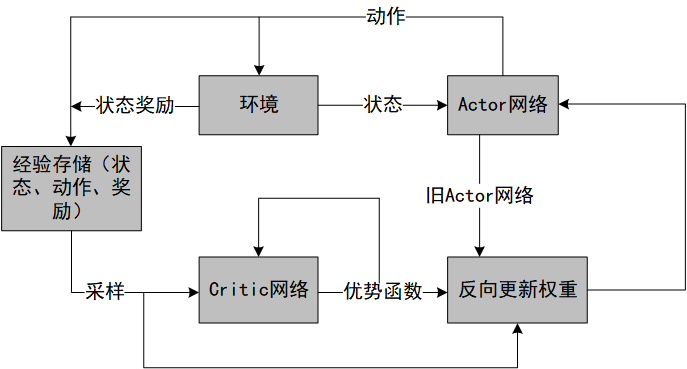
\includegraphics[width=0.75\textwidth]{figures/2.6}
	% \caption[这里的文字将会显示在 listoffigure 中]{这里的文字将会显示在正文中}
	\caption{PPO强化学习模型结构}\label{fig:2.6}
\end{figure}

\section{本章小结}

本章围绕ELF文件结构、恶意软件检测技术、对抗性恶意软件及强化学习四个方面展开了详细介绍。首先,从结构层面对ELF文件的基本组成进行了分析,重点阐述了ELF头、程序头表、节区及节头表在程序执行与加载过程中的作用。接着,介绍了当前主流的恶意软件检测技术,包括静态分析、动态行为分析以及基于机器学习和深度学习的方法,明确了各类方法的优劣和适用场景。在此基础上,进一步探讨了对抗性恶意软件的基本概念、生成方式及其对现有检测系统带来的挑战,指出对抗性样本具有极高的隐蔽性与攻击性,是当前研究中的热点难点问题。最后,本章简要回顾了强化学习的基本原理与流程,并结合恶意软件扰动任务,分析了其在对抗样本生成中的应用潜力。



%\chapter{基于强化学习的对抗性恶意软件生成技术架构 Adversarial Malware Generation Framework Based on Reinforcement Learning}
\section{研究的问题描述 Problem Researched Description}
近年来,随着深度学习在恶意软件检测领域的广泛应用,其高准确率与自动化能力极大提升了防御系统的智能化水平。然而,研究者相继发现深度神经网络存在严重的对抗性脆弱性——即对输入数据中微小扰动高度敏感,这些扰动在肉眼难以察觉的情况下,足以使模型输出完全错误的判断结果。这一特性被攻击者利用,催生出一种新型威胁形式:对抗性恶意软件。

In recent years, with deep learning widely adopted in malware detection, its high accuracy and automation capabilities have significantly enhanced defense systems’ intelligence. However, researchers have found that deep neural networks exhibit severe adversarial vulnerability, being extremely sensible to subtle disturbances in input data. Imperceptible to humans, these disturbances can cause models to produce entirely incorrect judgments. Attackers utilize this characteristic, catalyzing a novel threat: adversarial malware.

现有的对抗样本生成方法大多数集中于图像或文本等较为简单的数据类型。然而,在恶意软件领域,尤其是ELF文件等二进制可执行文件,扰动的设计和生成面临更多挑战。恶意软件的结构复杂且精密,任何不当的修改都可能导致文件失效或程序崩溃,因此,如何有效地生成既能绕过检测系统又能够保留恶意功能的对抗样本,是目前面临的核心问题。目前的对抗样本生成技术主要集中在静态和动态扰动上,但依然存在几个关键不足:

Current adversarial sample generation methods mostly focus on simpler data types like images or text. However, in malware realms, particularly for binary executables like ELF files, disturbance design faces greater challenges. Malware structures are so complex and precise that improper modifications may cause file failure or program crashes. Thus, how to generate adversarial samples that evade detection while ensuring malicious functionalities remains a crucial challenge. Current techniques mainly concentrate on static and dynamic disturbances but still exist critical shortcomings.

\begin{figure}[hbt]
	\centering
	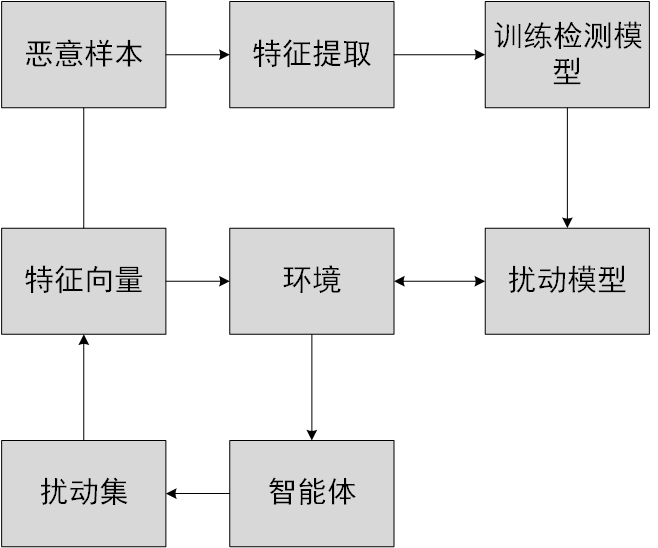
\includegraphics[width=0.75\textwidth]{figures/3.1}
	% \caption[这里的文字将会显示在 listoffigure 中]{这里的文字将会显示在正文中}
	\caption{常见对抗性恶意软件生成模型结构}\label{fig:3.1}
\end{figure}

\begin{enumerate} [label=\arabic*)] 

\item 扰动空间的局限性与复杂性 Limitations and Complexion in Disturbance Space

目前,针对对抗性恶意软件样本的生成,已有方法大多采用如字节插入、修改节区名称、篡改元数据等简单扰动手段来逃避检测系统,这类方法虽然操作便利、实现成本低,但往往缺乏结构感知与语义控制能力,其扰动维度较为单一,不能有效覆盖恶意软件在执行过程中所展现出的复杂特征。在面对复杂结构的二进制文件格式(如ELF)时,盲目扰动极易破坏文件原有逻辑或运行路径,导致样本功能失效或出现运行异常。此外,由于这类扰动方式通常在文件表层留下明显的痕迹,所生成的对抗样本容易被现代静态分析工具或启发式检测系统识别,且对抗效果往往不具备。稳定性和泛化能力。尤其在动态行为检测不断增强的背景下,如何在确保恶意功能完整的同时进行细粒度、多维度、良性扰动,成为当前对抗性样本生成研究中亟待突破的关键问题。

Existing methods for adversarial malware generation often rely on simplistic disturbances such as byte insertion, section name modification and metadata tampering, to evade detection. Although these methods are convenient to operate and are low cost, they lack structural awareness and semantic control capability. Besides, their disturbance dimensions are insufficient, which makes them hardly cover complex malware features efficiently during execution. For binary files that have intricate structure like ELF, disturbing blindly can easily disrupt file logic or execution paths, causing functional failure or abnormal behavior. Furthermore, such disturbance methods often leave obvious traces on file surfaces, making adversarial samples easily detected by modern static analysis or heuristic systems, which means the adversarial effectiveness lacks stability and generalizability. Especially in the background that dynamic behavioral detection is enhancing continuously, how to perform fine-grained, multi-dimensional and benign disturbances while ensuring functional integrity is a critical challenge to the research.

\item 扰动的合法性问题 Disturbance Legitimacy Problems

尽管当前部分对抗样本生成方法在规避恶意软件检测模型方面取得了一定成效,但其扰动策略普遍存在粗糙和随机性强的问题,常见手段包括随机字节插入、伪装节名称、修改冗余字段等浅层扰动。这类方法虽能在某些静态检测模型中绕过特征匹配机制,但缺乏对扰动合法性与语义一致性的有效控制,难以适应真实环境下多样化且复杂的检测机制。例如,随意插入的字节可能被高级检测模型识别为异常行为(如零号攻击),反而增强了恶意特征的可识别性。尤其对于依赖行为分析或异常检测的模型而言,盲目的扰动不仅无助于逃避检测,反而可能使模型学习到更具代表性的恶意特征,从而降低对抗攻击的有效性。此类“为扰动而扰动”的生成策略虽然可能在静态条件下取得短期成功,但难以保障在实际部署环境中的稳定性与隐蔽性。因此,如何构建更加结构化、具备语义感知能力的扰动策略,在不破坏原有功能的前提下提升扰动的针对性与有效性,成为当前对抗性恶意样本生成研究中的关键挑战之一。

Although current adversarial generation methods succeed in evading malware detection models, their disturbance strategies tend to be crude and highly random. Common operations include surface-level disturbances such as random byte insertion, disguised section names, and redundant byte modification. While features evade matching in static detectors, they lack effective control over disturbances legitimacy and semantic consistency, struggling against diverse real environments and detection mechanisms. For example, bytes inserted randomly may be recognized as abnormal behaviors such as zero-day attacks by advanced models, enhancing malicious feature detectability. Particularly for detection models based on behavior analysis or abnormal behavior detection, blind disturbances not only fail to evade detection but also risk teaching models more representative malicious features, reducing attack efficiency. Such strategies whose activities are only to disturb without considering effectiveness may achieve short-term static evasion but lack stability and concealment in a real deployment environment. Therefore, developing strategies that are more structural, high awareness to semantic to enhance precision and validity without losing origin functionalities is crucial.

\item 对历史扰动的依赖性缺失 Lacking Historical Disturbance Dependencies

对抗样本的生成过程本质上是一个动态决策序列,其扰动操作并非孤立发生,而是具有明显的时序依赖性——当前的扰动决策往往会受到先前扰动历史的影响。然而,现有的主流对抗样本生成方法大多将每一步扰动视为独立事件,缺乏对扰动序列内在依赖关系的建模与挖掘。这种近似于“无记忆”的策略忽略了扰动间的逻辑联系与语义上下文,导致生成的扰动序列在结构上缺乏连贯性,扰动操作之间相互脱节,甚至可能出现前后矛盾或重复无效的修改操作。这不仅降低了对抗样本的逃避能力和隐蔽性,还可能引入可疑的行为模式,反而提升被检测的风险。特别是在处理结构复杂、语义敏感的二进制恶意样本时,忽视扰动间依赖会进一步削弱攻击效果。因此,如何引入有效的时序建模机制,捕捉扰动操作之间的动态关联,从而生成更具整体性、策略性和欺骗性的扰动序列,是提升对抗样本实战能力的关键突破方向之一。

Adversarial sample generation is a dynamic decision-making sequence. Disturbance operations manifest sequential dependencies: current decisions depend on prior perturbation history, instead of isolation. However, prevalent methods treat each disturbance step as isolated, neglecting to find the inherent dependency relations. This approximately memoryless strategy ignores logical and semantic contexts between disturbances, resulting in generated sequences structural succession deficiency and disturbance operations disconnected from each other, which exhibits that some modification operations contradict with previous operations or duplicated. This result not only undermines adversarial samples’ evasion capabilities and concealment, but also potentially introduces suspicious action patterns that increase the detected rate. Especially in structurally complex, semantically sensitive malware binaries, overlooking the dependence between disturbances further reduces attack effectiveness. Therefore, introducing effective temporal modeling mechanisms to capture dynamic correlations in disturbance operations and generating more integral, strategic, deceptive disturbance sequences is a key breakthrough in enhancing adversarial sample capacities in real environments.

\item 过于关注逃逸率,忽视扰动成本与执行开销 Overemphasis on Evasion Rate and Negligence on the Cost of Execution

当前许多对抗性恶意软件生成方法普遍将“是否成功逃逸检测系统”作为主要评价指标,过度聚焦于误分类结果,而忽略了扰动过程中的多方面代价。在实际应用中,生成的对抗样本不仅需要具备较强的逃逸能力,还应兼顾扰动的实施成本与执行效率。例如,频繁或复杂的扰动操作可能导致样本体积显著增加、运行时间延长,甚至影响程序的原有功能和行为一致性,从而在实际环境中暴露风险。此外,部分策略在扰动选择上未考虑操作本身的资源消耗和可行性,导致生成的样本难以在有限计算资源下快速部署。忽视这些现实因素,往往使得对抗样本虽然能在检测模型层面绕过检查,但却在工程实际中难以落地。因此,仅以逃逸率为单一优化目标的生成策略存在明显局限,亟需引入对扰动成本与时间开销的系统性考量,以提升对抗样本的实用性与隐蔽性。

Many current adversarial malware methods mostly regard "successfully evading malware detection systems" as the primary evaluation metric, overemphasizing misclassification results while ignoring multifaceted costs of disturbance processes. However, in practical applications, not only high evasion capacities are required to adversarial samples generated, but also keeping the balance of implementation costs and execution efficiency. For example, excessive or complex disturbances significantly increase file size, prolong runtime, disrupt functionality, or affect behavioral consistency, which potentially exposes risks during execution. Furthermore, some strategies overlook resource consumption and feasibility of operations, rendering generated samples hard to deploy under constrained resources. Although ignoring these real-world factors allows samples to bypass detection models, it is a failure in engineering deployment. Therefore, the strategy that regards evasion rate as the only optimization exhibits significant limitations. It is urgent to introduce systemic consideration of disturbance costs and time to enhance sample practicality and concealment.

\end{enumerate}

本文主要的研究目的是借助强化学习和神经网络方法,构建多维度和高效的对抗样本生成方法。针对目前已有研究方法中存在的不足,本文提出以下需要解决的关键问题:

The primary objective of this research is to construct a multidimensional and efficient adversarial sample generation approach utilizing reinforcement learning and neural network methods. Addressing the shortcomings of existing methods, the following critical issues are required to resolve:

关键问题1:如何构建一个具备结构感知和语义控制能力的多维度扰动空间,以适应复杂恶意软件样本的逃逸需求?

Key Issue 1: How to construct a multidimensional disturbance space with structural awareness and semantic control capability to meet the evasion needs of complex malware samples?

关键问题2:如何提升扰动的合法性与良性,避免传统“破坏式扰动”在真实检测系统中反而暴露攻击意图?

Key Issue 2: How to enhance disturbance legitimacy and benignity, avoiding traditional "destructive disturbances" that may expose attack intentions in real detection systems?

关键问题3:如何引入扰动历史建模机制,从而生成更具连贯性和策略性的扰动序列?

Key Issue 3: How to introduce historical disturbance modeling mechanisms to generate more coherent and strategic disturbance sequences?

关键问题4:如何在对抗样本生成过程中权衡扰动有效性、功能完整性与资源开销,提升攻击样本的实际可部署性?

Key Issue 4: How to balance effectiveness, functional integrity, and resource consumption during adversarial sample generation to enhance the practical deployability of attack samples?

\section{研究的设计思路 Research Design Logic}
针对当前对抗性恶意软件样本生成方法在扰动手段粗糙、语义控制能力弱、扰动序列缺乏结构性以及忽视现实成本与可部署性等方面的不足,本文提出了一种创新的对抗样本生成框架。现有方法通常依赖简单且随机的字节插入、修改节名称等手段,缺乏对生成样本的合法性、语义一致性以及可执行性的有效控制,导致在实际环境中难以稳定有效地逃避检测。因此,本文的研究思路旨在通过系统性地优化对抗样本生成的多个关键方面,弥补这些不足。

To address current adversarial malware generation methods' limitations in coarse perturbation techniques, weak semantic control, lack of structural disturbance sequences, and neglect of practical costs and deployability, this research proposes an innovative adversarial sample generation framework. Common existing methods rely on simple, random byte insertions or section name modifications that lack effective control over sample legitimacy, semantic consistency, and executability, resulting in unstable evasion in real environments. Therefore, this research aims to solve these shortcomings by systematically optimizing multiple key aspects of adversarial sample generation.

首先,在扰动空间建模方面,本文通过引入多维度扰动技术,打破了传统方法只依赖单一扰动手段的局限,考虑到恶意软件在不同执行阶段可能展现出的多样化特征,设计了一种结构化且具有语义感知能力的扰动策略,从而避免了对文件功能的破坏,同时提高了逃避检测的难度。其次,针对扰动合法性问题,本文提出了一种基于语义一致性的扰动合法性控制方法,确保生成的对抗样本在避开检测的同时,能够维持原有的功能和行为一致性,避免了盲目扰动所带来的不稳定性。

Firstly, in the disturbance space modeling aspect, this paper introduces multidimensional disturbance techniques and breaks the limitation of traditional methods that solely rely on single disturbance methods. Since malware exhibits diverse features in different execution stages, this research designs a structural disturbance strategy with semantic awareness capacities, avoiding file functionality disruption and enhancing evasion difficulties. Secondly, targeting the disturbance legitimacy issue, a disturbance legitimacy control method based on semantic consistency is proposed to ensure adversarial samples evade detection while maintaining original functionality and behavioral consistency, avoiding instability from blind disturbances.

另外,考虑到对抗样本生成过程中的扰动序列具有明显的时序依赖性,本文通过强化学习中的PPO算法结合LSTM网络对扰动序列进行建模,从而有效捕捉扰动操作之间的动态关系,使得生成的扰动序列在整体上更加连贯、隐蔽和具备欺骗性。通过这一方法,能够优化扰动的执行顺序和策略,进一步提升对抗样本的逃避能力。

Furthermore, recognizing the obvious temporal dependency in disturbance sequences, this research employs the PPO algorithm combined with LSTM networks to model disturbance sequences, effectively capturing dynamic relationships between disturbances. This approach enhances the overall coherence, stealth, and deceptive nature of disturbance sequences, optimizing the order and strategies to further improve evasion capabilities.

最后,针对现有方法忽视扰动过程中的成本与可执行性问题,本文提出了一种新的奖励机制,除了关注检测逃逸率外,还考虑了生成过程中的资源消耗、执行时间等因素,确保生成的对抗样本不仅具备较高的攻击性,还能够在实际环境中顺利部署,避免因过于复杂的扰动操作导致样本体积膨胀、运行时间延长或功能丧失。

Lastly, addressing the neglect of disturbance costs and executability, a new reward mechanism is proposed in this research. Except for focusing on evasion rates, it considers different factors such as resource consumption and execution time, ensuring that adversarial samples are not only highly aggressive but also deployable in real environments. This prevents sample size surges, prolonged runtime, or functional loss caused by excessive disturbances.

与传统方法相比,本文具有以下几个显著优点:

\begin{enumerate} [label=\arabic*)] 

\item 结构感知的扰动空间构建:突破以往依赖静态规则或单一字节操作的扰动方式,本文在样本的结构层与语义层中引入更细粒度的操作集,设计出支持多维度、多粒度扰动的操作空间,能够更精准地定位关键行为区域并施加微扰动,从而有效提升逃避检测的灵活性和有效性。

Structurally Aware Perturbation Space Construction: Departing from previous disturbance methods relying on static rules or single-byte operations, this research introduces a finer-grained operation set at the structural and semantic layers of samples, designing an operational space supporting multidimensional and multigranular disturbances, enabling to localize key behavioral regions more precisely and apply subtle disturbances, thereby effectively enhancing the flexibility and effectiveness of evasion detection.

\item 扰动合法性与语义一致性的融合控制机制:不同于以往“只求误判、不管后果”的扰动逻辑,本文在生成过程中引入语义保持约束与合法性验证策略,确保扰动不会破坏程序原有逻辑与可执行性,从而提升对抗样本在真实系统中的稳定性与隐蔽性。

Fusion Control Mechanism for Disturbance Legitimacy and Semantic Consistency: Unlike the previous disturbance logic that only pursues misclassification regardless of consequences, this research incorporates semantic preservation constraints and legitimacy verification strategies during the generation process, which ensures that disturbances do not disrupt the original program logic and executability, enhancing the stability and concealment of adversarial samples in real systems.

\item 考虑扰动历史的序列建模机制:本文将对抗扰动过程视为一个具有时序依赖特征的策略优化任务,引入序列建模机制(如记忆单元或策略网络)来捕捉扰动操作之间的上下文关系,使生成的扰动序列更具策略性与一致性,解决了以往扰动碎片化、冗余化的问题。

Sequence Modeling Mechanism Considering Disturbance History: This research regards the adversarial disturbance process as a strategy optimization task that exhibits temporal dependency characteristics. It introduces sequence modeling mechanisms, such as memory cells or policy networks, to capture the contextual relationships between disturbance operations, which enables the sequences generated to be more strategic and consistent, addressing the previous issues that disturbances are fragmented and redundant.

\item 面向成本与开销的实用性优化目标:本文在对抗目标设计中充分考虑扰动的实施成本、样本运行效率和部署风险等实际因素,引入“轻量扰动”与“开销评估”机制,有效控制扰动规模和复杂度,使生成样本更具工程实用性,避免“虽逃逸成功却难以部署”的局限。

Optimization Objective Oriented towards Cost and Overhead Practicality: In designing the adversarial objectives, this research fully considers practical factors such as disturbance implementation cost, sample runtime efficiency, and deployment risk, introducing "lightweight perturbation" and "overhead assessment" mechanisms to effectively control the scale and complexity of disturbances. This makes the samples generated more practical for engineering deployment, thus avoiding the limitation of being evasive but hard to deploy.

\end{enumerate}

\section{研究的解决方案 Research Solutions}

针对本文3.1节中当前对抗性恶意软件样本生成方法中存在的扰动手段粗糙、语义控制能力弱、扰动序列缺乏结构性以及忽视现实成本与可部署性等问题,本文提出了一种面向实用性与隐蔽性强化的对抗样本生成框架。该框架从多个维度出发,提出了四个关键解决方案,以提高对抗样本的生成能力、逃避检测效果及实用性。

To address the issues in Section 3.1—that disturbance methods are coarse, weak semantic control, lack of structural disturbance sequences, and neglect practical costs and deployability—this paper proposes a novel adversarial sample generation framework facing practicality and concealment enhancement. This framework focuses on enhancing generation capabilities, evasion effectiveness, and practicality through 4 key solutions.

解决方案1:基于多维度的扰动空间建模

Solution 1: Disturbance Space Modeling Based on Multi-dimensions

传统的对抗样本生成方法通常采用简单的扰动方式,如字节插入、节区名称修改、冗余字段篡改等,这些方法虽然在短期内能够绕过检测,但其扰动空间较为有限,无法有效应对恶意软件复杂执行过程中的多样化特征。为此,本文提出了一种多维度扰动策略,通过精确建模多种扰动维度,从结构、指令、行为三个层面对扰动空间建模以全面覆盖恶意软件在执行过程中可能展现出的行为特征。该策略能够有效提高恶意软件样本的逃避能力和隐蔽性,同时保持样本的功能完整性。在扰动设计中,特别关注对恶意代码执行路径、控制流及其他关键结构的精确干扰,从而最大程度避免传统方法中存在的结构损坏和功能失效的问题。

Traditional adversarial sample generation methods usually employ simple disturbances, such as byte insertion, section name modification, or redundant byte modifications. While these methods may temporarily evade detection, their disturbance space is limited, failing to address the diverse features exhibited during malware execution. To address this issue, this paper proposes a multidimensional perturbation strategy. By precisely modeling various disturbance dimensions, this approach constructs a disturbance space across structural, instruction, and behavioral layers, comprehensively covering potential behavioral features during malware execution. This strategy enhances the evasion and concealment capabilities of malicious samples while preserving their functional integrity. Disturbance design particularly targets precise interference with malicious code execution paths, control flows, and other critical structures, minimizing structural damage and functional failure issues in traditional methods.

解决方案2:基于良性样本的合理化插入扰动

Solution 2: Rationalized Insertion Disturbance Based on Benign Samples

当前许多对抗样本生成方法的扰动通常依赖于随机字节插入等浅层操作,这种方式缺乏对语义合法性和扰动合理性的控制,容易导致生成样本的不稳定性或被检测到。为了解决这一问题,本文提出了一种基于良性样本的合理插入扰动方法。在这一方法中,首先通过分析良性样本的结构与行为,提取出良性样本的语义与字节结构,构建良性样本扰动库。通过对扰动进行更加结构化和语义感知的设计,保证了对抗样本在功能上的完整性和合法性,同时减少了不必要的噪声扰动。这种方法不仅能有效规避基于特征匹配的静态检测系统,还能增强对抗样本在复杂检测环境中的隐蔽性。

Current adversarial sample generation methods often rely on shallow operations, such as random byte insertion, lacking control over semantic legitimacy and disturbance rationality. This can lead samples to be unstable and to be detected easily. To overcome this disadvantage, this paper introduces a rationalized insertion disturbance method based on benign samples. By analyzing the structure and behavior of benign samples, their semantic and byte structure are extracted to build a benign sample perturbation library. This method ensures functional completeness and legitimacy of adversarial samples through more structurally and semantically aware disturbance design, reducing unnecessary noise. It not only effectively evades static detection systems based on feature matching but also enhances sample concealment in complex detection environments.

解决方案3:基于LSTM的PPO时序依赖建模

Solution 3: PPO Temporal Dependency Modeling Based on LSTM

对抗样本的生成不仅仅是每一步独立的扰动操作,而是一个具有时序依赖性的过程。现有方法通常忽略了扰动间的依赖关系,导致生成的扰动序列缺乏整体性和连贯性,从而影响逃避能力。为了解决这一问题,本文结合PPO\cite{yu2022surprising}(Proximal Policy Optimization)强化学习算法和LSTM\cite{graves2012long}(Long Short-Term Memory)模型,提出了一个联合优化的时序依赖建模方法。通过LSTM网络对扰动序列的时序关系进行建模,捕捉扰动之间的内在依赖性,PPO算法则用于优化生成策略。这一方法能够生成更具整体性、连贯性和隐蔽性的扰动序列,有效提升对抗样本的攻击性和稳定性。

Adversarial sample generation is not merely a series of independent disturbances but a process with temporal dependencies. Existing methods often overlook dependencies among different disturbances, resulting in disjointed sequences and reduced evasion capabilities. To solve this issue, this paper combines the PPO Reinforcement Learning algorithm\cite{yu2022surprising} with LSTM\cite{graves2012long} models to propose a joint optimization method for temporal dependency modeling. LSTM networks model temporal relationships in disturbance sequences, capturing intrinsic dependencies among disturbance operations, while PPO optimizes generation strategies. This method produces holistic, coherent, and stealthy disturbance sequences, enhancing adversarial sample attack effectiveness and stability.

解决方案4:基于动态奖励函数的智能体决策

Solution 4: Decision-Making Agent Based on Dynamic Reward Functions

在现有的对抗样本生成方法中,奖励函数设计往往过于简单,通常只关注样本是否成功绕过检测系统,而忽略了生成过程中的成本与效率问题。为了克服这一不足,本文提出了一种基于动态奖励函数的智能体决策机制。该机制不仅考虑逃逸成功与误分类率,还引入了扰动的资源消耗、执行效率、时间开销等因素。通过这种动态奖励机制,智能体在决策过程中能够更好地平衡攻击性与执行代价,从而生成既具备高隐蔽性,又能够快速部署的对抗样本。该方法有效提升了对抗样本的实际应用价值和部署可行性。

Existing adversarial sample generation methods often employ simplistic reward functions focused solely on whether the sample evades the detection systems, neglecting generation costs and efficiency. To address this disadvantage, this research proposes an agent-making mechanism based on dynamic reward functions. Beyond considering evasion success and misclassification rates, it incorporates factors, such as disturbance resource consumption, execution efficiency, and time costs. This dynamic reward mechanism enables agents to balance attack effectiveness with execution costs during decision-making, generating adversarial samples that are both highly stealthy and quickly deployable. This approach significantly enhances the practical application value and deployability of adversarial samples.

\section{研究的整体架构  Research Overall Framework}

为了有效应对恶意软件检测系统的不断演进,提升对抗样本在真实环境下的生存能力与攻击效果,本文提出了一套系统化的对抗样本生成架构。整体设计遵循分层递进、策略引导、效果评估的原则,涵盖了数据收集、扰动策略建模、强化学习智能体训练以及奖励函数设计等关键环节,确保对抗样本能够在保证功能正确性的前提下,最大程度逃逸各类检测系统的拦截。

To effectively address evolving malware detection systems and enhance the survivability and attack effectiveness of adversarial samples in real environments, this research proposes a systematic adversarial sample generation framework.Its overall design follows principles of hierarchical progression, strategy guidance, and effect evaluation and contains key components, such as data collection, disturbance strategy modeling, RL agent training, and reward function design, ensuring adversarial samples maximize evasion rate across various detection systems while maintaining functional correctness.

%\begin{enumerate} [label=(\arabic*)] 

(1) 数据收集与预处理

(1) Data Collection and Preprocessing

高质量的数据基础是对抗样本生成系统有效运行的关键前提,尤其是在针对ELF格式可执行文件的研究中,由于当前尚缺乏权威性、标准化的公开数据集,这一问题尤为突出。为弥补该空白,本文自主构建了一个覆盖面广、结构多样的ELF样本集,涵盖恶意样本与正常样本两个维度,确保后续模型训练与扰动策略评估具有良好的实验基础与推广能力。

High-quality data is fundamental to the adversarial sample generation system effective operation, especially dominant for ELF-format executable file research due to the current lack of authoritative, standardized public datasets. To bridge this gap, this research constructs a full-coverage, structurally diverse ELF sample set, including both malicious and benign samples, ensuring a robust experimental foundation and promotion capability for model training and disturbance strategy evaluation.

在恶意样本采集方面,本文主要从VirusShare\cite{VirusShare}、Maltrieve等知名的开源恶意软件平台中筛选并下载经过多重验证的x86架构下的ELF格式恶意样本。样本类型涵盖多种常见攻击形式,包括蠕虫传播程序、加密货币挖矿程序、远程控制型后门程序、DDoS工具及嵌入式木马等,具有较强的代表性与研究价值。为进一步提升样本质量,本文对收集到的样本进行了格式校验、哈希去重、恶意行为标签确认等预处理操作,确保样本集的真实性与一致性。在正常样本采集方面,本文基于QEMU虚拟化技术搭建了多个目标运行环境,主要包括基于Raspbian和OpenWrt的ARM架构嵌入式系统,以及基于Ubuntu的x86系统环境,从中提取了系统默认运行的合法ELF程序,如系统工具、守护进程、配置脚本等。这些样本在功能完备、结构规范的同时,能够覆盖多种开发工具链和构建方式,进一步增强了正常样本集的多样性与代表性。

For malicious sample collection in this research, verified ELF-format malware samples targeting x86 architecture were sifted and downloaded from renowned open-source platforms such as VirusShare\cite{VirusShare} and Maltrieve. These samples cover common attack types, such as worm propagation programs, cryptocurrency miners, remote-controlled backdoors, DDoS tools, and embedded Trojans, offering strong representativeness and research value. To enhance sample quality, format validation, duplicate hash removal, and malicious behavior label verification were performed to ensure authenticity and consistency.For benign sample collection in this research, multiple target runtime environments were established using QEMU virtualization technology, including ARM-based embedded systems like Raspbian and OpenWrt, and x86-based systems like Ubuntu. Legitimate ELF programs, such as system tools, daemons, and configuration scripts were extracted from those embedded systems. These samples, being functionally complete and structurally standard, cover various development tool chains and build methods, enhancing the diversity and representativeness of the benign sample set.

为了确保数据集的质量与准确性,本文在完成初步样本收集后,针对所有获取的ELF格式可执行文件样本均引入了VirusTotal\cite{VirusTotal}平台的复审机制,以增强样本标注的权威性与恶意性确认的可信度。具体而言,首先对每个样本执行SHA-256等哈希指纹提取操作,构建唯一标识,剔除重复或冗余的样本项,确保样本集的去重和纯净;随后将样本上传至VirusTotal平台,通过其集成的多引擎病毒扫描系统(涵盖Kaspersky、Avast、BitDefender、ESET等多个主流安全厂商)进行全面检测。

To ensure dataset quality and accuracy, after initial sample collection, a review mechanism from the VirusTotal\cite{VirusTotal} platform was introduced for all collected ELF executable samples, strengthening the authority of label notes annotation and the credibility of maliciousness confirmation. In detail, first, hash fingerprints like SHA-256 are extracted from each sample to create unique identifiers, removing duplicate and redundant samples. Second, samples are uploaded to VirusTotal for comprehensive detection by using integrated multiple engines that contain Kaspersky, Avast, BitDefender, and ESET. 

在扫描过程中,本文重点关注引擎返回的检测标签、恶意评分(malicious score)、行为分析结果以及YARA规则匹配情况等关键信息,构建每个样本对应的检测报告元数据集,用于后续的分析、训练与评估。同时,对于存在标注不一致或引擎分歧较大的边界样本,通过引入手动复审或多轮投票方式进一步判断其可信分类,保证数据标注的一致性和准确性。
此外,扫描报告中所提取的信息(如API调用特征、连接行为、时间戳等)也为后续的扰动操作设计与对抗样本生成提供了参考依据,帮助理解当前主流检测机制所侧重的关键特征,从而指导扰动策略选择。

In the scanning process, this research concentrates on critical information, including detection tags, malicious scores, behavioral analysis results and YARA rule matches returned by engines, which are used to construct a metadata report for each sample for subsequent analysis, training and evaluation. Besides, manual review and multi-round voting are introduced to judge and classify marginal samples that exhibit annotation inconsistency or significant engine disagreements, ensuring data annotation consistency and accuracy. Furthermore, information extracted from the scan reports, such as API call signatures, connection behaviors, and timestamps, also serves as a reference for subsequent disturbance design and adversarial sample generation, helping to identify key features prioritized by current detection mechanisms and guiding disturbance strategy selection.

(2)扰动策略构建

(2) Disturbance Strategy Construction

针对现代恶意软件检测系统在静态、动态以及行为特征等多维度的集成分析机制,本文提出了一种具有分层次特征的组合式扰动策略,旨在从结构信息、指令序列和动态行为三个层面入手,打破传统特征提取链条,从而提升对抗样本的隐蔽性与鲁棒性。在现有检测系统中,往往通过固定规则或训练模型提取静态特征(如节结构、函数调用图、符号信息)、指令级特征(如n-gram、CFG路径)以及动态行为(如系统调用序列、内存行为等),因此,设计能够有效扰乱这些检测路径的扰动机制对于生成高质量对抗样本具有重要意义。

To counter modern malware detection systems' integrated analysis across static, dynamic, and behavioral features, this research proposes a hierarchical combined disturbance strategy that targets to disrupt traditional feature extraction chains through three levels—structural information, instruction sequences, and dynamic behaviors, enhancing the concealment and robustness of adversarial samples. Since current detection systems typically rely on fixed rules or trained models to extract static features, such as section structures, function call graphs, symbol info, instruction-level features, such as n-grams and CFG paths, and dynamic behaviors such as system call sequences, memory behaviors, thus, designing disturbance mechanisms effective against these detection paths is crucial for generating high-quality adversarial samples.

在结构扰动方面,本文主要采用插入式结构变换策略,该策略具有较好的通用性和对原程序功能的非破坏性。具体方法包括在ELF二进制文件中插入伪造节(section)和无效段(segment),例如通过LIEF库\cite{LIEF2025}动态创建.fake、.dummy\_code等节,且这些节不参与程序逻辑流程,仅作为混淆成分存在;同时对ELF头部(ELF Header)、程序头表(Program Header Table)及节区头表(Section Header Table)进行轻量修改,如调整节表顺序、伪造入口点地址、添加重定位信息等,使得静态分析工具在解析时产生偏差。此外,还包括对程序进行壳处理(packing)和脱壳(unpacking)操作,通过UPX等压缩工具实现结构扰动,并结合反壳策略恢复执行能力,从而扰乱基于字节签名和结构模式匹配的检测系统。

In structural disturbance aspect, this research mainly adopts structural transformation strategies based on insertion that exhibit high adaptivity and are not disruptive to original program functionalities. Concrete methods include inserting fake sections and invalid segments in ELF binary files, such as dynamically create sections that are only used for obfuscation and do not engage program logic processes, such as .fake and .dummy\_code, by using LIEF \cite{LIEF2025} library. Additionally, slight ELF Header, Program Header Table and Section Header Table adjustments, including altering section table sequences, fabricating the entry point address and adding relocation information, induce parsing errors in static analysis tools. Furthermore, packing and unpacking structural disturbance operations via compression tools like UPX, along with strategies to restore execution capability, confuse detection systems based on byte signature and structural pattern comparison. 

\begin{figure}[hbt]
	\centering
	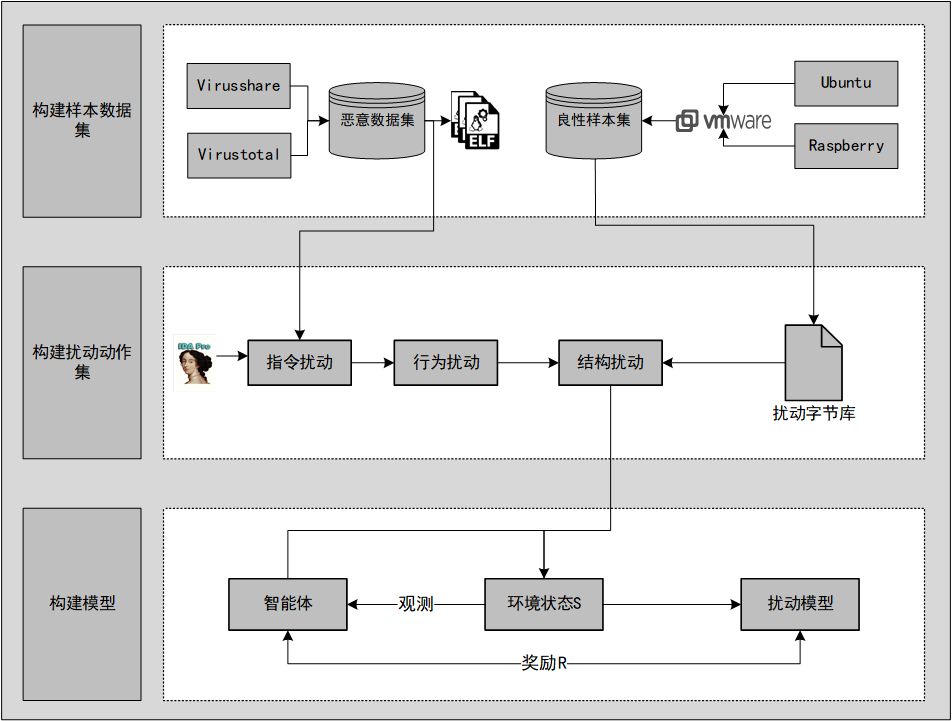
\includegraphics[width=0.75\textwidth]{figures/3.2}
	% \caption[这里的文字将会显示在 listoffigure 中]{这里的文字将会显示在正文中}
	\caption{基于强化学习的对抗性样本生成方法框架}\label{fig:3.2}
\end{figure}


在指令层面,本文通过结合IDA Pro、radare2等反汇编工具,对原始二进制样本进行静态反汇编与控制流图提取,进而实现对指令的扰动式重写。首先,在保证程序语义不变的前提下,使用等价指令替换技术,例如用xor eax, eax替换mov eax, 0,或使用冗余的加法/减法指令链完成简单赋值,扰乱检测模型对常规语义的理解;其次,利用寄存器交换策略(如将eax换为ebx等)打破寄存器使用模式,同时修改跳转指令逻辑,在跳转目标不变的情况下引入间接跳转、中间跳板、无效跳转等手段,以此增加CFG的复杂度,干扰以控制流为特征的静态图分析器。在指令组合上,本文还引入了无效填充操作,如NOP滑块(NOP sled)与空函数调用序列,进一步加大模型提取有效语义片段的难度。

In the instruction layer, this research used disassembly tools, such as IDA Pro and radare2, to disassemble original binary samples and extract control flow graphs to achieve instruction disturbance. First, in the background that program semantics are not disrupted, equivalent instruction replacements, such as using “xor eax, eax” to replace “mov eax, 0” and using redundant arithmetic chains to achieve simple assignments, disturb common semantic understanding for detection models. Second, utilizing register swapping strategies like replacing “eax” with “ebx” changes register usage patterns and modifies instruction jump logic. Indirect jumps and invalid jumps are introduced to increase CFG complexity to disturb static diagram analyzer targeted on CFG features with the premise that jump target is not changed. In the instruction combination realm, this research introduces invalid padding operations, such as NOP sled and empty function call sequences, to increase the difficulty of extracting meaningful semantic segments.

针对动态分析系统的行为建模特性,本文设计了一套动态执行扰动机制,旨在规避基于沙箱技术的行为检测模型。该机制通过修改程序实际入口点(Entry Point),优先执行伪造行为逻辑,再逐步过渡到真实恶意载荷执行,从而在短时间行为采集窗口中有效延迟真实行为暴露。常用策略包括添加自循环逻辑(例如构造伪循环结构)、空跳转路径(无逻辑变化但执行时间延长)以及插入系统级延迟调用,如sleep()、nanosleep()等API,来阻断沙箱的行为提取流程。此外,还可嵌入虚拟环境检测语句(如CPUID指令、MAC地址识别等),使得样本在虚拟分析平台上呈现不同行为路径,进一步规避检测。结合动态段的无效控制流插入,本文的扰动策略在沙箱动态行为分析阶段展现出良好的逃避性能。

To address dynamic analysis system behavioral model features, this research design a dynamic execution disturbance mechanism aims to evade behavioral detection models based on sandbox techniques. This mechanism modifies the actual Entry Point, prioritizes executing fabricated behavioral logic and then gradually executes true malicious code, effectively postponing the exposure of factual behaviors in windows that capture behaviors. Common strategies include self-loop logic, such as fabricated loop structures, empty jump paths that do not affect program execution logic but prolong execution time and delayed APIs insertions, such as sleep() and nanosleep(), which prevent sandbox extraction workflows. Furthermore, virtual environment detection functions, such as CPUID instructions and MAC address identification instructions, can also be embedded to make samples exhibit different behaviors on platform based on virtual analysis. Combined with inserting invalid control flows into dynamic segments, these disturbance strategies demonstrate strong evasion capabilities during dynamic behavior analysis based on sandboxes.

(3)奖励函数策略优化

(3) Reward Function Strategy Optimization

在本研究中,强化学习(RL)模型的奖励函数设计是生成对抗性恶意软件样本的核心要素之一。为了使智能体能够有效地避开恶意软件检测系统,并生成具有足够复杂性的对抗样本,本文提出了一种综合考虑检测逃逸、样本多样性和生成复杂度的奖励函数。奖励函数的优化与构建直接决定了智能体在训练过程中的学习效果和最终生成的恶意样本的质量。

In this research, designing the reward function for the RL model is a core element for generating adversarial malware samples. To enable the agent to effectively evade malware detection systems and generate adversarial samples with sufficient complexity, this research proposes a reward function that comprehensively considers evasion success, sample diversity, and generation complexity. The optimization and construction of the reward function directly determine the agent's learning effectiveness during training and final generated malicious samples' quality.

首先,奖励函数的主要目标是鼓励智能体生成能够避开现有检测系统的恶意样本。因此,奖励函数首先根据样本是否能够逃避检测来给予奖励。当智能体生成的样本未被恶意软件检测模型判定为恶意时,智能体将获得一个正向奖励,反之则给予负向奖励。这个反馈机制可以引导智能体在生成过程中不断优化策略,以提高恶意样本的逃逸能力。

First, the primary goal of the reward function is to encourage the agent to generate malicious samples that can evade existing detection systems. Therefore, the reward function grants rewards based on whether the sample successfully evades detection. When the sample generated by the agent is not classified as malicious by the malware detection model, the agent receives a positive reward; otherwise, it receives a negative reward. This feedback mechanism guides the agent to continuously optimize its strategy during generation, thereby improving the evasion capability of malicious samples.

其次,样本的多样性也是奖励函数中一个重要的考虑因素。在对抗性样本生成过程中,若智能体能够通过修改程序的控制流、修改函数调用顺序、插入随机字符串等方式增加样本的多样性,将会获得相应的奖励。通过这种方式,奖励函数促进了恶意样本的多样化,避免了模型生成过于单一或重复的样本,从而提高了生成样本的泛化能力。

Second, sample diversity is also a critical factor that should be considered in the reward function. During adversarial sample generation process, if the agent increases sample diversity by modifying control flow, altering function call sequences, or inserting random strings, it receives corresponding rewards. This approach promotes the diversification of malicious samples, avoids generating monotonous or duplicate samples, and enhances the generalization ability of generated samples.

最后,为了避免智能体在生成样本时产生过于复杂或不稳定的结果,本文在奖励函数中引入了对样本复杂度的惩罚机制。当生成的恶意样本过于复杂(例如,通过过多的控制流操作或冗长的代码片段),智能体将受到一定的惩罚。这一策略帮助智能体在保证逃逸能力的同时,生成更加稳定和有效的样本,从而提高生成的样本的实际应用价值。

Finally, to prevent the agent from generating overly complex or unstable results, the reward function incorporates a penalty mechanism for sample complexity. If a generated malicious sample is excessively complex, such as containing too many control flow operations or lengthy code fragments, the agent is penalized. This strategy helps the agent generate more stable and effective samples while ensuring evasion capability and enhancing the practical application value of generated samples.

为了使奖励函数更加灵活和适应不同训练阶段,本文还采用了动态调整策略。在训练的初期,智能体主要依赖于探索奖励,通过多样化的变异操作来探索不同的恶意样本类型。随着训练的进展,探索奖励逐步减少,智能体将更多地依赖于利用已知的优秀策略,以生成更加高效和复杂的恶意样本。这种动态调整机制确保了智能体能够在探索和利用之间找到平衡,并逐步提升生成样本的质量。

To make the reward function more flexible and adaptable to different training phases, this research adopts a dynamic adjustment strategy. In the initial training phase, the agent primarily relies on exploration rewards to explore diverse mutation operations and generate various malicious sample types. As training progresses, exploration rewards gradually decrease, and the agent increasingly relies on known effective strategies to generate more efficient and complex malicious samples. This dynamic adjustment ensures that the agent finds a balance between exploration and exploitation, progressively improving the quality of generated samples.

(4)强化学习模型构建与训练

(4) Reinforcement Learning Model Construction and Training

在前述模型架构中,本文设计了强化学习的智能体,旨在通过持续优化恶意软件样本生成过程以规避检测。为了提升智能体的决策能力和生成样本的多样性,本文采用了LSTM和PPO相结合的强化学习模型。

In the model structure proposed previously, this research designs a RL agent aimed at continuously optimizing the malware sample generation process to evade detection. To enhance the agent's decision-making capability and the diversity of generated samples, this research adopts an RL model combining LSTM and PPO.

首先,LSTM被集成到智能体的策略网络中,以便捕捉生成过程中的长期依赖关系。恶意软件样本的生成过程通常是序列化的,每一步生成的行为不仅依赖于当前的输入,还受到之前生成步骤的影响。LSTM作为一种循环神经网络,能够有效存储并利用这些历史信息,从而增强模型在生成恶意样本时的准确性和灵活性。通过这种方式,智能体能够在执行每一个生成操作时考虑到先前的生成状态,进而做出更加合理的决策,减少生成结果的不一致性。

First, LSTM is integrated into the agent's policy network to capture long-term dependencies in the generation process. Malware sample generation is commonly sequential. Each generation step depends not only on the current input but also on prior steps. As a recurrent neural network, LSTM effectively stores and utilizes historical information, enhancing the accuracy and flexibility of the model during malware generation. This solution enables the agent to consider previous generation states when performing each operation, make more reasonable decisions and reduce inconsistencies in generated results.

在此基础上,PPO强化学习算法被用来进一步优化策略的更新过程。PPO作为一种近端策略优化方法,利用了较为稳定的策略更新机制,有效避免了策略的剧烈波动。通过控制每次策略更新的幅度,PPO能够保证智能体在不断尝试和学习的过程中,既能够快速提高生成效果,又能避免由于过度优化而导致的不稳定。PPO通过对策略网络的不断优化,使得智能体能够逐步学会如何在恶意软件生成过程中最大化逃避检测系统的概率,从而提高生成样本的攻击性和隐蔽性。

On this basis, the PPO RL algorithm is used to optimize the policy update process further. As a proximal policy optimization method, PPO adopts a stable update mechanism, effectively avoiding severe policy fluctuations. By controlling the magnitude of each policy update, PPO ensures the agent rapidly improves generation performance while preventing the model from being unstable due to over-optimization. Through PPO continuously optimizing the policy network, the agent can progressively learn how to maximize evasion probability against detection systems during malware generation, thereby enhancing the aggressiveness and concealment of generated samples.

在训练过程中,智能体每生成一个恶意软件样本,就会根据检测模型给出的评分作为奖励反馈给智能体。这些奖励信号作为训练的动力,推动策略网络的优化。为了增强训练的稳定性,本文采用了经验回放机制和奖励归一化技术。这些方法使得智能体在学习过程中能够更加高效地利用过去的经验,同时避免由于奖励过大或过小导致学习不平衡的情况。

During the training process, each time the agent generates a malware sample, the detection model's evaluation is provided as feedback to the agent. These rewards serve as training incentives to promote strategy network optimization. To enhance training stability, this research employs an experience replay mechanism and reward normalization techniques that enable the agent to utilize past experiences more efficiently and prevent learning imbalance from excessively large or small rewards.

通过这种结合LSTM和PPO的方法,智能体能够在恶意软件生成任务中不断优化其生成策略。最终,训练完成的模型能够生成具有高度复杂性和隐蔽性的恶意软件样本,这些样本能够有效地避开现有的恶意软件检测系统,提升了对抗性样本生成的能力。

Through this method combining LSTM and PPO, the agent continuously optimizes its generation strategies for malware generation tasks. Ultimately, the trained model can generate highly complex and stealthy malware samples that effectively evade current malware detection systems, significantly advancing adversarial sample generation capabilities.

%\end{enumerate}
\section{本章小结 Chapter Summary}

本章首先介绍了当前恶意软件检测领域中面临的挑战,特别是在应对新型对抗性样本时,传统的检测方法往往无法有效识别。通过分析现有技术的不足之处,发现许多传统方法所存在的问题。针对这些问题,本章提出了对应的解决方案。接下来,本章详细介绍了这一解决方案的设计思路。通过强化学习算法,代理能够在训练环境中与检测模型互动,学习如何生成绕过检测的恶意样本。这一过程通过奖励机制引导代理生成具有高隐蔽性和变异性的样本,从而提升恶意软件的复杂度和变化性,使得现有的检测方法更难识别。最后,本章描述了整个系统的整体架构设计。该架构包括数据收集与处理、扰动策略构建、奖励函数策略优化与强化学习模型构建与训练四个部分以实现本文的研究目标,完成对抗样本的生成。

First, this chapter introduces the challenges faced in the malware detection realm, particularly the severe condition that traditional malware detection methods are ineffective at detecting novel adversarial samples. Through an analysis of existing techniques, many shortcomings existing in traditional methods are pointed out. To address current technology issues, this chapter presents corresponding solutions. It then provides detailed design logic for these solutions. By adopting reinforcement learning algorithms, the agent interacts with detection models in a training environment to learn how to generate malicious samples that can evade detection. This process is guided by reward mechanisms that encourage the agent to generate highly stealthy and variable samples to enhance malware complexity and variability, making it harder for existing detection methods to identify them. Finally, the chapter describes the overall system architecture that comprises four key components: data collection and processing, disturbance strategy construction, reward function strategy optimization, and RL model construction and training. This architecture is designed to achieve the research target, successfully generating adversarial samples.
%\chapter{基于强化学习的对抗性恶意软件生成方法研究方案 Research Solution for Adversarial Malware Generation Technology Based on Reinforcement Learning}

本章将具体地介绍本文提出的对抗样本生成方法的详细设计过程和实现原理,主要包括扰动方法的构建,奖励函数策略的设计,模型的具体结构。

This chapter will specifically introduce the detailed design process and implementation principles of the adversarial sample generation method proposed in this research, which mainly includes disturbance methods' construction, the reward function strategies' design, and the model's specific structure.

\section{多维度扰动方法的构建 Multidimensional Disturbance Methods' Construction}

本文利用lief库、IDA pro对二进制可执行样本进行批量处理。LIEF(Library to Instrument Executable Formats)是一个开源的库,用于处理ELF、PE和Mach-O格式的可执行文件。它可以解析和修改二进制文件的头部信息、节区、符号和动态链接。LIEF适用于静态分析、重命名符号、插入代码和文件格式转换等任务。LIEF可以提取二进制可执行文件的结构,以及提供各个结构的操作接口。

This research batch processes binary executable samples using the LIEF library and IDA Pro. LIEF (Library to Instrument Executable Formats) is an open-source library for processing executable files in ELF, PE, and Mach-O formats. It can parse and modify header information, sections, symbols, and dynamic linking in binary files. LIEF is applicable to tasks such as static analysis, symbol renaming, code insertion, and file format conversion. LIEF can extract the structure of binary executable files and provide operation interfaces for various components.

\subsection{结构化扰动方法 Structural Disturbance Methods}

在恶意软件的对抗性样本生成过程中,结构层面的扰动指的是通过修改文件的内部结构来引入变化,这种变化通常不会影响文件的执行逻辑,但能够有效地逃避传统的检测方法。结构层面的扰动包括但不限于文件的节区、导入符号、动态库、以及压缩/解压缩等操作。

In the adversarial malware sample generation process, structural level disturbances refer to introducing changes by modifying a file's internal structure. These changes commonly do not affect the file's execution logic but effectively evade traditional detection methods. Structural level disturbances include operations on sections, imported symbols, dynamic libraries, compression, and decompression, but are not limited to these.

这些扰动主要关注的是通过改变文件结构中的某些元素来达到以下目的:

These disturbances primarily concentrate on achieving the following purposes by altering certain elements in the file structure:

增加文件的不可预测性:通过随机化或改变文件的某些部分,使得检测系统很难依赖固定模式进行识别。

Increasing file unpredictability: By randomizing or changing parts of the file, detection systems hardly identify the file, relying on fixed patterns.

避开静态分析:静态分析工具通常依赖文件的固定结构特征,如节区(Section)、符号表、导入表等。通过扰动这些结构,可以增加检测的难度。

Evading static analysis: Static analysis tools often depend on fixed file structural features, such as sections, symbol tables, and import tables. Disturbing these structures increases detection difficulty.

防止签名匹配:一些恶意软件检测工具依赖于已知恶意样本的特征(如哈希值、节区结构等)进行匹配。通过扰动结构,可以使文件与原始恶意样本在这些特征上产生差异,从而避开检测。

Avoiding signature matching: Some malware detection tools rely on known signatures, such as values, section structures from malicious samples. Disturbing structures creates differences between the file and the original malicious sample in these signatures, enabling evasion.

(1)节区(Section)扰动

(1) Section Disturbance

在ELF(Executable and Linkable Format)文件中,节区是文件的基本构建单元。它们存储了不同类型的数据(如代码、数据、符号等)。通过对节区内容进行扰动,可以修改文件的行为或使其变得更加复杂。常见的节区扰动方式包括:

In ELF files, sections are the fundamental units, storing different types of data, such as code, data, symbols. Disturbing section content can modify file behavior or increase its complexity. Common section perturbation methods include:

节区内容的修改:例如,在现有节区中附加随机数据、将特定节区的数据替换为 benign 数据(如无害的字符串或二进制内容)等。这样可以增加恶意文件的复杂性并避免与已知恶意样本的特征匹配。

Modifying section content: For example, appending random data to existing sections or replacing data in specific sections with benign data like harmless strings or binary content increases malicious files’ complexity and avoids matching known malicious sample signatures.

节区重命名:将节区名称修改为常见的名称或随机名称,使得检测工具无法轻易识别文件中的关键节区,如 .text 节区,通常包含程序代码。

Renaming sections: Changing section names to common or random names makes it harder for detection tools to identify critical sections, especially the .text section that contains program code.

本文设计的节区扰动如表\ref{tab:4.1}所示。

The section disturbance design in this paper is listed in Table \ref{tab:4.1}.

\begin{table}[htbp]
	\centering
	\caption{节区扰动类型}\label{tab:4.1}
	\begin{tabular*}{\textwidth}{@{\extracolsep{\fill}}ccc}
		\toprule
		扰动 & 简写 & 效果 \\
		\midrule
		section\_append & SA & 向随机选择的节中追加随机数据(可能改变节的内容和熵) \\
		add\_section\_benign\_data & ASBD & 从 benign 文件中提取整个节,并添加到目标 ELF 中 \\
		add\_section\_strings & ASS & 生成一个新的节,填充 benign 字符串内容 \\
		section\_rename & SR & 随机重命名一个节,使用常见节名列表中的名称 \\
		\bottomrule
	\end{tabular*}
\end{table}

(2)导入符号和库扰动

(2) Imported Symbol and Library Disturbance

ELF文件中的导入符号表(dynamic symbol table)包含了程序运行时需要链接的外部函数或库。通过扰动这些符号,可以使恶意软件的行为更加不可预测。例如:

The dynamic symbol table in ELF files contains external functions or libraries that require runtime linking. Disturbing these symbols can make malware behavior more unpredictable. For example:

添加恶意符号:将恶意的动态符号(如恶意函数名)添加到文件中,或者通过与良性文件进行符号混合,增加文件的复杂性。

Adding malicious symbols: Inserting malicious dynamic symbols such as malicious function names into the file or mixing symbols with benign files to increase complexity.

修改库依赖:修改ELF文件所依赖的动态库,使其依赖于一个不存在或不常见的库,从而打乱传统的静态分析过程。

Modifying library dependencies: Altering ELF dependency libraries that do not exist or are not common disrupts traditional static analysis processes.

本文设计的导入符号和库扰动如表\ref{tab:4.2}所示。

The imported symbol and library disturbances designed in this paper are listed in Table \ref{tab:4.2}.

\begin{table}[htbp]
	\centering
	\caption{导入符号和库扰动}\label{tab:4.2}
	\begin{tabular*}{\textwidth}{@{\extracolsep{\fill}}ccc}
		\toprule
		扰动方法 & 简写 & 效果 \\
		\midrule
		add\_imports & AI & 从 benign ELF 文件中添加一个动态符号到目标 ELF 中(如函数导入) \\
		add\_library & AL & 从 benign ELF 文件中添加一个共享库和其导入函数 \\
		\bottomrule
	\end{tabular*}
\end{table}


(3)随机数据附加(Overlay)

(3) Random Data Appending (Overlay)

Overlay技术通过在文件末尾添加随机数据(通常是无害数据或伪装数据),可以在不改变文件执行流程的情况下修改文件的大小和结构。这种技术常用于恶意软件中以绕过基于签名的检测。常见的技术包括:

Overlay techniques involve appending random data that is commonly harmless or disguised to the end of a file, altering its size and structure without changing execution logic. This technique is commonly used in malware to evade detection based on signature comparison. Common methods include:

追加随机字节:将随机的字节序列附加到ELF文件的末尾。此操作不会影响文件的执行逻辑,但可能会改变文件的哈希值,使其避开传统的哈希匹配检测。

Appending random bytes: Adding random byte sequences to the end of ELF files. This operation does not affect execution logic but may change file hashes, making the file evade traditional detection based on hash comparison.

追加无害二进制文件内容:从已知的良性文件中提取节区或二进制内容,插入到恶意文件中,以增加文件的复杂度并扰乱静态分析工具的检测。

Appending benign binary content: Inserting sections or binary content extracted from known benign files into malicious file increases complexity and disrupts static analysis tool detection.

\begin{table}[htbp]
	\centering
	\caption{随机数据附加类型}\label{tab:4.3}
	\begin{tabular*}{\textwidth}{@{\extracolsep{\fill}}ccc}
		\toprule
		扰动方法 & 简写 & 效果 \\
		\midrule
		overlay\_append & OA & 在二进制文件的末尾附加随机内容 \\
		append\_benign\_data\_overlay & ABDO & 追加来自 benign ELF 文件 .text 段的内容 \\
		append\_benign\_binary\_overlay & ABBO & 直接追加整个 benign ELF 文件内容 \\
		add\_strings\_to\_overlay & ASTO & 追加来自 benign 字符串文件的内容(UTF-8 编码) \\
		\bottomrule
	\end{tabular*}
\end{table}

(4)压缩与解压缩(UPX打包与解包)

(4) Compression and Decompression (UPX Packing and Unpacking)

压缩恶意文件是另一种常见的扰动技术。通过使用UPX等压缩工具对ELF文件进行压缩,可以隐藏文件的原始结构,并使文件在未经解压时不可执行。这种方法主要有以下特点:

Compressing malicious files is another common disturbance technique. Compressing ELF files using tools like UPX can hide the original file structure and make the file non-executable without decompression. This approach primarily has the following features:

压缩:压缩文件可以改变文件的内部结构,使其看起来与原始文件完全不同,从而避开基于特征的检测。

Compression: Compressed files alter the file's internal structure, making it appear entirely different from the original, thereby evading detection based on features.

解压缩:压缩的ELF文件在运行时会被解压缩回原始状态,因此需要额外的解压步骤。通过这种方式,恶意软件的行为和文件结构可以被“隐藏”在压缩层后面,增加了反向工程和静态分析的难度。

Decompression: Compressed ELF files are decompressed to their original state during runtime, requiring an additional decompression step. This method allows malicious software behaviors and file structures to be hidden behind the compression layer, increasing the difficulty of reverse engineering and static analysis.

\begin{table}[htbp]
	\centering
	\caption{压缩加壳类型}\label{tab:4.4}
	\begin{tabular*}{0.9\textwidth}{@{\extracolsep{\fill}}ccc}
		\toprule
		扰动方法 & 简写 & 效果 \\
		\midrule
		upx\_pack & UP & 使用 upx 对 ELF 文件进行压缩 \\
		upx\_unpack & UUP & 使用 upx -d 解压已压缩的 ELF 文件 \\
		\bottomrule
	\end{tabular*}
\end{table}

(5)Go语言的go-bindata工具包装ELF文件

(5) go-bindata Toolbox in Go for Packaging ELF Files

go-bindata是一个Go工具,旨在将二进制文件(如ELF文件、图片、音频文件等)转化为Go源代码中的字节数组。在恶意软件分析领域,通过将ELF文件嵌入到Go程序中,可以有效隐藏ELF文件的实际内容,并增加静态分析和反向工程的难度。具体而言,go\_bindata\_wrapper方法通过将ELF文件转换为Go代码,实现在Go程序中隐藏ELF文件的功能。这种方式使得恶意文件能够避开常规的静态检测和签名匹配工具。

go-bindata is a Go tool designed to convert binary files, such as ELF files, images, and audio files, into byte arrays within Go source code. In the malware analysis realm, embedding ELF files into Go programs effectively conceals their actual content and increases the difficulty of static analysis and reverse engineering. Specifically, the go\_bindata\_wrapper method converts ELF files into Go code to hide their functionalities in Go programs, which enables malicious files to evade common static detection and signature-matching tools.

go-bindata工具的作用:go-bindata工具将任何二进制文件(如ELF文件)嵌入到Go源代码中,并生成一个包含文件内容的Go文件。在程序运行时,生成的Go文件将包含文件的字节数组,这些字节数据可以被Go程序读取,并用于恢复原始文件内容。此方法使得ELF文件内容隐藏在Go源代码中,从而增加了恶意软件在反向工程过程中的隐蔽性。

Function of the go-bindata tool: The go-bindata tool embeds any binary file like ELF files into Go source code, generating a Go file containing the file's content. When the file is executed, this generated Go file includes a byte array that the Go program can read to recover the original file's content. This method hides ELF file content in Go source code, enhancing the concealment of malware during reverse engineering.

通过go-bindata工具将ELF文件转换为Go源代码,并生成一个Go文件,Go文件中包含该ELF文件的字节数据。通过Go编译器将包含ELF文件字节数据的Go代码编译成最终的Go可执行文件。ELF文件在运行时会被读取并恢复,执行原始文件的操作。

First, convert the ELF file into Go source code using the go-bindata tool, generating a Go file containing the ELF file's byte data. Then, compile this Go code that contains the ELF byte data into a final Go executable program using the Go compiler. At runtime, the ELF file is read and recovered to execute its original operations.

通过go-bindata工具,go\_bindata\_wrapper方法为恶意文件提供了一种新的隐蔽方式,将ELF文件嵌入到Go程序中,从而有效地规避静态分析工具和签名匹配的检测。

Through the go-bindata tool, the go\_bindata\_wrapper method provides a novel concealment approach for malicious files by embedding ELF files into Go programs, thus effectively evading static analysis tools detection and signature matching.

(6)节头表修改

(6) Section Header Table Modification

节头表扰动旨在通过修改二进制文件中的特定元数据或表头信息,从而改变其表象特征,扰乱检测工具或逆向分析过程。这种技术常用于恶意软件分析中的对抗样本生成,目的是使恶意程序绕过传统的反病毒软件或沙箱检测系统,增加分析难度。\ref{tab:4.5}介绍了本文使用的两种节头表扰动方法。

The target of section header table disturbances is altering the apparent characteristics of binary files by modifying specific metadata or header information, thereby disrupting detection tools or reverse analysis processes. This technique is commonly used in adversarial sample generation for malware analysis, aiming to help malicious programs evade traditional antivirus software or sandbox detection systems and increase analysis difficulty. Figure \ref{tab:4.5} introduces two section header table disturbance methods adopted in this paper.

\begin{table}[htbp]
	\centering
	\caption{节头表扰动类型}\label{tab:4.5}
	\begin{tabular*}{0.9\textwidth}{@{\extracolsep{\fill}}ccc}
		\toprule
		扰动方法 & 简写 & 效果 \\
		\midrule
		Remove Debug & RD & 在二进制文件中删除调试信息(用零填充) \\
		Break Checksum & BC & 在可选标题中删除校验和值(用零填充) \\
		\bottomrule
	\end{tabular*}
\end{table}

\subsection{指令扰动方法 Instruction Disturbance Methods}

在本研究中,本文使用强大的反汇编工具 IDA Pro 对 ELF 格式的恶意软件样本进行静态分析与代码提取,为后续的语义保持扰动操作奠定基础。尽管对于剥离符号信息(如符号表、调试信息)的 x86 架构 ELF 可执行文件,难以做到完全精确的反汇编,但现有的高级反汇编器(如 IDA Pro)已可通过多种技术手段对主流编译器生成的代码实现较高覆盖率。这些手段包括:多种反汇编算法的结合使用、对特定代码结构的识别、以及简单的数据流分析等。在处理 ELF 文件时,IDA Pro 通过识别符号信息和程序头表中的节区(如 .text、.plt、.rela.plt 等),能够较准确地定位函数边界,识别控制流,并生成基本块图和函数调用图,帮助提取语义稳定的指令区域进行变换。

In this research, powerful disassembly tools like IDA Pro are adopted to perform static analysis and code extraction on ELF-format malware samples, establishing a foundation for subsequent disturbance operations that ensure semantics. Although achieving fully precise disassembly remains challenging for stripped symbols like missing symbol tables and debugging information ELF executables on x86 architecture, advanced current disassemblers like IDA Pro can achieve high coverage for code generated from prevalent compilers through combined disassembly algorithms, recognition of specific code structures, and basic data-flow analysis. When processing ELF files, IDA Pro identifies symbol information and sections in the Program Header Table, such as .text, .plt, .rela, and .plt, enabling locating function boundaries accurately, recognizing control flow, and generating basic block graphs and function call graphs. This facilitates the extraction of semantically stable instruction regions for transformation.

\begin{figure}[hbt]
	\centering
	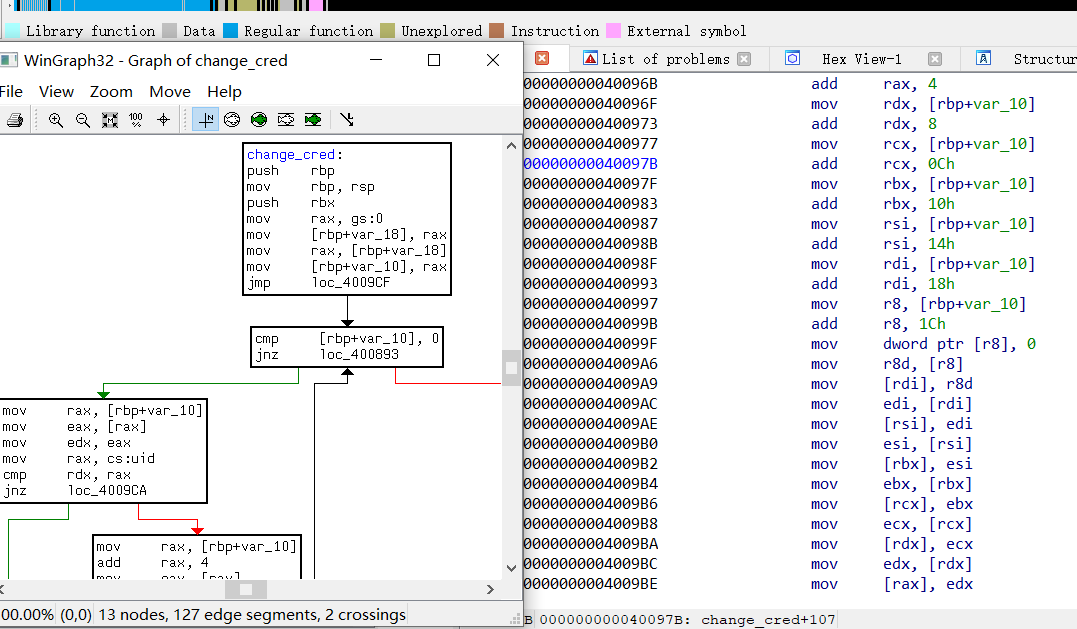
\includegraphics[width=0.75\textwidth]{figures/4.1}
	% \caption[这里的文字将会显示在 listoffigure 中]{这里的文字将会显示在正文中}
	\caption{IDA 反汇编 CFG 图}\label{fig:4.1}
\end{figure}


为确保扰动操作不影响原始程序逻辑,本文首先将反汇编得到的指令转换为一种自定义的中间表示(IR),该表示能记录每条指令的操作码、显式与隐式操作数、寄存器读写关系、以及影响到的标志位等静态语义信息。这种增强表示形式可有效辅助分析控制依赖与数据依赖关系,识别出可安全修改的指令区域。随后,本文实施三种语义保持的扰动技术:指令替换(Instruction Substitution)、指令重排序(Instruction Reordering) 和 寄存器重分配(Register Reallocation)。这三类方法分别从指令级别、顺序层级和寄存器使用层面引入扰动,旨在保持语义不变的前提下实现样本多样性和模型鲁棒性提升。

To ensure disturbances do not disrupt the original program logic, the disassembled instructions are first transformed into a custom Intermediate Representation (IR). This IR records each instruction's static semantic information, such as opcode, explicit and implicit operands, register read and write relationships, and impacted flag bits, which effectively aids in analyzing control and data dependencies to identify safely modifiable instruction regions. Subsequently, three disturbance techniques—Instruction Substitution, Instruction Reordering, and Register Reallocation—ensure semantics are implemented. These methods respectively introduce disturbances at the instruction level, sequential layer, and register usage level, aiming to enhance sample diversity and model robustness while preserving semantics.

在变换过程中,所有修改操作均限制在已识别的、无控制依赖冲突的基本块内部,确保程序控制流图(CFG)保持稳定。如果某些变换操作(如指令顺序调整)导致代码地址偏移,本文会同步更新 ELF 文件中的相关重定位信息(如 .rela.text 段),以避免函数调用或跳转地址错误。整个扰动流程针对每个 ELF 文件独立执行,可自动生成多个等价但具有不同语法表现的扰动样本,用于训练或测试阶段的多样化增强,从而有效提升基于静态分析的恶意代码检测系统的鲁棒性。

During transformation, all modifications are limited to identified basic blocks free of control dependency conflicts, ensuring Program Control Flow Graph (CFG) stability. If transformations like instruction resequencing cause code address shifts, relevant relocation information, such as .rela section and .text section, in the ELF file is synchronously updated to prevent faulty function call and jump address. This process executes per ELF file independently, automatically generating multiple syntactically distinct yet semantically equivalent adversarial samples. These enhance diversity in training and testing phases, effectively improving the robustness of malware detection systems based on static analysis.

(1) 指令替换(Instruction Substitution)

(1) Instruction Substitution

指令替换作为一种二进制代码扰动方法,旨在通过将原始指令替换为等效的指令来扰乱程序的结构,同时保持程序的功能不变。该方法不仅能改变代码的外观,还能增加静态分析和逆向工程的难度。以下是指令替换的具体细节:

Instruction substitution serves as a binary code disturbance method that alters program structure by replacing original instructions with equivalent ones while preserving program functionality. It not only disrupts code appearance but also increases the difficulty for static analysis and reverse engineering. Details are described as follows:

等效指令替换:

Equivalent Instruction Replacement:

在x86架构中,许多指令有多个等效形式,可以用不同的操作数或指令格式来实现相同的功能。例如:
add r/m32, r32 可以替换为 add r32, r/m32,这两者在操作数为寄存器时是等效的。

On x86 architecture, many instructions have multiple equivalent forms, same functionality can be achieved by different operands and instruction forms.For example, “add r/m32, r32” can be replaced with “add r32, r/m32”, these two instructions are equivalent while operands are registers.

对于逻辑操作,test r/m8, r8 可以与 test r/m8, r/m8 等价。

For logic operations, “test r/m8, r8” is equivalent to “test r/m8, r/m8”.

一些算术指令也有多个等效形式,比如 sub r/m32, r32 可以用 neg r/m32 替换(减法可以通过取负来实现)。

Some arithmetic instructions also have multiple equivalent forms, such as “sub r/m32, r32” can be replaced with “neg r/m32”.

操作数形式替换指令时,可以改变操作数的形式,而不影响最终的计算结果。例如,mov r32, r/m32 和 mov r/m32, r32 都是等效的操作,但通过改变源和目标操作数的顺序,能够改变指令的字节表示。

Operand forms can be altered when instructions are replaced, and do not affect ultimate calculation result. For example, “mov r32, r/m32” and “mov r/m32, r32” are equivalent operations, but the instruction byte expression can be altered by changing the sequence of source and target operands.

不同长度指令某些情况下,可以用长度相同但操作不同的指令替换原始指令,例如:
inc r32可以替换为 add r32, 1,二者功能相同,但指令长度和编码不同。

In some circumstances, replacing original instructions with instructions that are the same length but different in operations are permitted.
For example, “inc r32” can be replaced with “add r32, 1”, these two instructions have same functionality, different instruction length and coding.

dec r32可以替换为 sub r32, 1,实现同样的效果,增加了代码的复杂性。

“dec r32” can be replaced with “sub r32, 1”, these two instructions have same effect, but increase code's complexity.

替换控制流指令:

Control Flow Instruction Replacement:

控制流指令(如跳转、条件跳转、调用等)也可以用等效的指令替换。例如:
jmp label 可以用 call label; pop 来替换,虽然实现了相同的跳转效果,但操作数和指令形式不同。

Control flow instructions, such as jump, conditional jump, and call, can be replaced with equivalent instructions. For example, “jmp label” can be replaced with “call label; pop”, although two instructions achieve same jump result, but their operands and instruction forms are different.

je(等于跳转)可以替换为 jne(不等于跳转),并通过适当调整标志位来维持功能一致性。

“je” can be replaced with “jne” by adjusting the flags properly to maintain functional consistency.

确保指令长度一致:

Maintain instruction length consistency:

由于对于许多stripped二进制文件,增加指令长度可能会导致代码结构破坏,因此在替换过程中要保证每条替换的指令与原指令长度相同。可以通过选择长度一致的等效指令来实现这一点,避免扰乱程序的整体布局。

Increasing instruction length may cause code structure to be broken in many stripped binary files; thus, it is vital to ensure that each replaced instruction's length should be the same as the original. This can be achieved by selecting equivalent instructions that have the same length, avoiding disrupting the program's overall layout.

随机化替换的应用方式:

The application method of randomized replacement:

在替换指令时,可以根据一定的规则或随机选择等效指令来应用这些替换。替换不一定是对每条指令都应用,而是根据程序的特性和分析结果,选择性地对特定代码块进行替换。这种方法可以确保替换不会影响程序的控制流和逻辑结构,但同时会改变程序的外观,增加静态分析的难度。

Replacements can be applied according to certain rules or randomized equivalent instruction selection. Replacements may not be applied to each instruction but are selectively applied to specific code blocks relying on program characteristics and analysis results. This method can ensure that replacements do not affect the program's control flow and logic structure but alter the program's appearance, increasing static analysis difficulty.

通过以上方法,指令替换不仅保持程序功能的完整性,还有效增加了程序的混淆性,使得静态分析工具更难识别程序的真实意图,增加了逆向工程的复杂性。

Through the methods above, instruction replacements not only maintain the program's complete functionalities but also increase the program's obfuscation, making it harder for static analysis tools to recognize the program's real intention and increasing the complexity of reverse engineering.

(2)指令重排序(Instruction Reordering)

(2) Instruction Reordering

基本块内部指令重排(Intra Basic Block Reordering):

Intra Basic Block Reordering:

在一个基本块(Basic Block)中,若两条或多条指令之间没有数据或控制依赖关系,那么它们的执行顺序就是可以互换的。由于基本块是线性执行的中间代码区域,并且编译器在生成机器码时只是选择了若干等效顺序之一,因此只要保证依赖关系不变,修改指令顺序不会影响程序的功能。

In a basic block, instructions without data and control dependencies can be reordered without affecting functionality. Since basic blocks are intermediate code areas for linear execution, and the compiler only selects one of equivalent sequences during machine code generation, thus instruction sequence modification does not affect the program's functionality if the dependency relationship remains unchanged.

本文对目标二进制程序进行反汇编,提取所有基本块。对每个基本块进行依赖分析,识别每条指令的读(use)和写(def)寄存器集。通过检测读后写(RAW)、写后读(WAR)、写后写(WAW)等依赖类型,构建出指令间的有向无环图(DAG)。

This research disassembles target binaries to extract all basic blocks, then perform dependency analysis on each block, identifying each instruction's use and def register sets, constructing a Directed Acyclic Graph (DAG) among instructions by detecting RAW (Read-After-Write), WAR (Write-After-Read), and WAW (Write-After-Write) dependencies.

之后,使用拓扑排序枚举该图的合法指令顺序,并从中随机选取一种新的顺序,替代原始顺序。这一方法不会引入新的指令或修改指令操作数,因此保持程序的功能完全不变。它可以扰乱基于指令顺序或特征码的静态分析和检测机制,有效提升样本的多样性。

Subsequently, this research enumerates legal instruction orders via topological sorting and randomly selects a new order to replace the original. This method can maintain the program's functionality because it does not introduce any new instructions or modify instruction operands. It disrupts static analysis mechanisms relying on instruction order or signatures, enhancing sample diversity.

\begin{figure}[hbt]
	\centering
	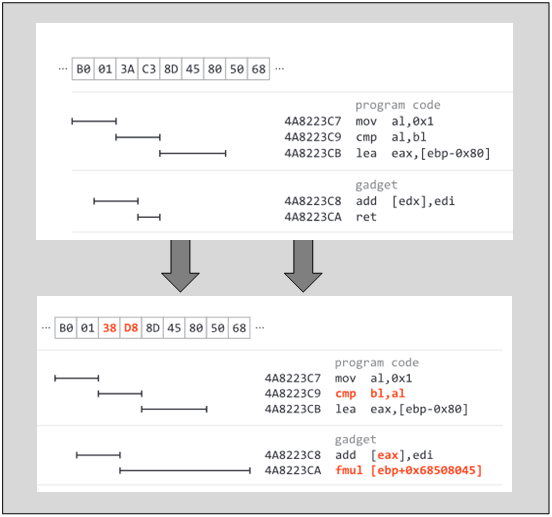
\includegraphics[width=0.75\textwidth]{figures/4.2}
	% \caption[这里的文字将会显示在 listoffigure 中]{这里的文字将会显示在正文中}
	\caption{指令替换示例图}\label{fig:4.2}
\end{figure}

寄存器保护代码重排(Reordering of Register Preservation Code):

Reordering of Register Preservation Code:

该方法基于函数调用时保存非易失性寄存器(callee-saved registers)所使用的push和pop指令的顺序是可变的,只要遵循“先进后出”的栈规则即可。即,函数在开头会使用若干push指令保存寄存器,函数结尾使用对应的pop恢复值。因为栈是倒序恢复的,所以只要保持pop顺序与push顺序相反,整个过程的语义就是等效的。

This method is based on the theory that the sequence of push and pop instructions from callee-saved registers is alterable during function calls, which only need to follow the last-in-first-out (LIFO) stack rule. During function calls, the order of push (callee-saved registers) and corresponding pop instructions can vary if adhering to the last-in-first-out (LIFO) stack rule. Several push instructions are used by the function header to save data in registers, while corresponding pop instructions are used at the end of the function to restore values. Since the stack restores in reverse order, semantics during the entire process will be equivalent to the original if pop sequences are the opposite of push sequences.

本文在函数的入口和出口识别出完整的寄存器保存/恢复代码段。对这些push和pop指令进行配对,确认其保护的是相同的寄存器,并追踪栈指针(ESP)的变化确保没有中间干扰。然后,对push序列进行重排,并将pop序列同步做相反的重排,确保恢复顺序正确。若push序列中夹杂有其他非保存性指令,也需进行依赖分析,保证重排不会打乱依赖顺序。这种方法对程序语义无影响,但能干扰基于特定pop序列模式的分析方法,提高静态分析、指令特征提取和样本分类的复杂度。

This research identifies complete register save and restore code segments at the function entry and exit. Then pair push and pop instructions, ensuring that they operate on the same registers and track ESP changes to avoid other interference. Subsequently, reordering the push sequence and applying inverse reordering to pop sequence ensures restore proper sequence. If the push sequence contains other non-preservation instructions, dependency analysis is also essential to ensure that reordering does not disrupt dependency sequence. This method has no impact on the program's semantics but disturbs analysis methods based on specific pop sequence patterns, improving resistance to static analysis, instruction feature extraction, and classification.

\begin{figure}[hbt]
	\centering
	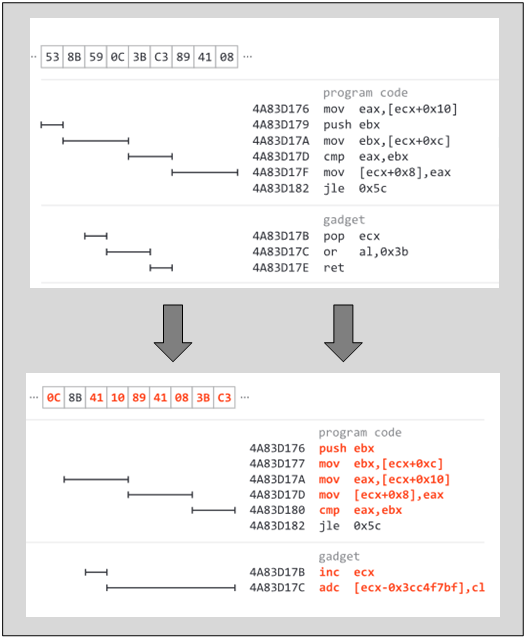
\includegraphics[width=0.75\textwidth]{figures/4.3}
	% \caption[这里的文字将会显示在 listoffigure 中]{这里的文字将会显示在正文中}
	\caption{指令重构排序示例图}\label{fig:4.3}
\end{figure}

\begin{figure}[hbt]
	\centering
	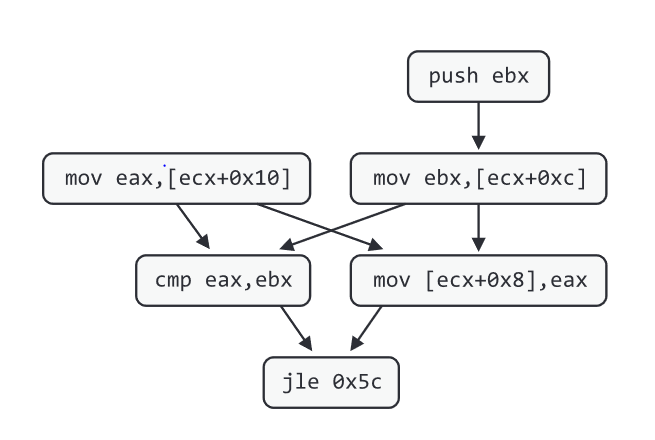
\includegraphics[width=0.75\textwidth]{figures/4.4}
	% \caption[这里的文字将会显示在 listoffigure 中]{这里的文字将会显示在正文中}
	\caption{重构的指令有序无环图}\label{fig:4.4}
\end{figure}

\begin{figure}[hbt]
	\centering
	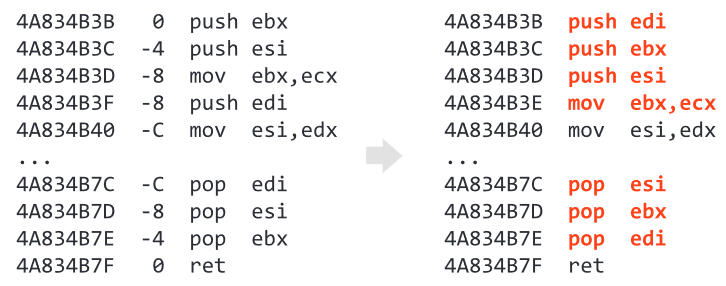
\includegraphics[width=0.75\textwidth]{figures/4.5}
	% \caption[这里的文字将会显示在 listoffigure 中]{这里的文字将会显示在正文中}
	\caption{寄存器保护代码重排序示例图}\label{fig:4.5}
\end{figure}

本文首先对二进制程序构建控制流图(CFG),并对每个基本块进行寄存器活跃性分析,获取每条指令的寄存器use(使用)与def(定义)集合。接着迭代计算每条指令的活跃输入集(in)与输出集(out),识别每个寄存器的活跃区域。在确保无冲突的前提下,随机选择两个不重叠活跃区的寄存器对,将其在汇编中的使用位置进行替换。指令修改时,通过变更ModR/M字节(必要时SIB字节)实现重映射,避免使用esp等特殊寄存器,并对隐式使用寄存器的指令进行过滤。为保证调用一致性,还需结合调用约定信息约束某些寄存器的使用。

First, this method constructs the CFG for the binary program and performs register liveness analysis on each basic block to determine each instruction's register use and def sets. Second, this method iteratively computes each instruction's active in and out sets to identify live ranges in each register. On the premise that there is no conflict, two register pairs with non-overlapping live ranges are randomly selected, and then their usage positions are swapped in assembly. During instruction modification, modifying via ModR/M bytes (and SIB bytes if necessary) achieve remapping, avoiding special registers like ESP, filtering instructions with implicit register usage. To ensure call consistency, calling convention information is combined to constrain certain registers.

这一方法不会引入新指令或修改操作数值,仅在机器码层面更换寄存器编号,因此程序行为保持完全一致。该技术能有效打乱静态分析工具基于寄存器使用模式或特征序列的识别策略,从而提升样本的对抗性与多样性。

This technique does not introduce any new instructions or change operand values, modifying only register encodings at the machine-code level. It disrupts static analysis tools based on register usage patterns or feature sequences recognition strategies, enhancing sample adversariality and diversity.

\begin{figure}[hbt]
	\centering
	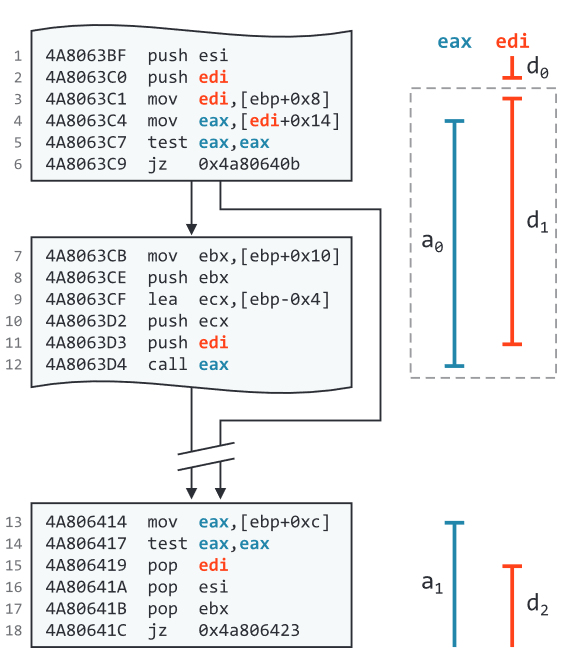
\includegraphics[width=0.75\textwidth]{figures/4.6}
	% \caption[这里的文字将会显示在 listoffigure 中]{这里的文字将会显示在正文中}
	\caption{寄存器重分配示例图}\label{fig:4.6}
\end{figure}

\subsection{动态行为扰动方法 Dynamic Behavior Disturbance Methods}

在恶意软件检测领域,动态分析技术是当前主流手段之一,尤其在处理未知样本或多态变种时具有明显优势。其基本原理是通过在受控执行环境(如沙箱、虚拟机、内存监控器)中运行目标程序,记录其在运行过程中所触发的系统调用、行为路径、内存修改、网络通信等信息,以此识别潜在的恶意行为。然而,这一技术在实际部署中往往存在时间资源受限的问题。为了兼顾效率与成本,动态分析系统通常仅为每个样本分配数秒到几十秒的执行时间窗口。对于某些攻击行为触发依赖于条件判断、用户交互的恶意样本而言,这一固定的分析时间窗显然存在被规避的可能性。

In the malware detection realm, dynamic analysis technology is one of the currently prevalent approaches, demonstrating clear advantages when handling unknown or polymorphic variants. Its fundamental principle involves running target programs in controlled execution environments, such as sandboxes, virtual machines, and memory monitors, recording triggered system calls, behavioral paths, memory modifications, network communications, and other runtime information to identify potential malicious behaviors. However, this technology often faces time and resource constraints during deployment. To balance efficiency and cost, dynamic analysis systems commonly allocate only a few seconds to dozens of seconds of execution time to each sample. For malware whose attack behaviors depend on conditional triggers or user interaction, this fixed analysis window presents a probability of being evaded.

基于此观察,本文设计了一种动态扰动方法,核心思想是引入“时间延迟”机制,使恶意代码在样本启动后故意等待一段时间再执行核心逻辑,从而躲避沙箱的行为分析窗口。其主要实现方式是通过在程序入口点或关键路径中插入延迟逻辑(如 nanosleep系统调用),使恶意样本在运行初期不表现任何异常行为,从而骗过基于行为特征的检测系统。

Based on this observation, this research designs a dynamic disturbance method whose central mechanism is introducing "time-delay", deliberately waiting for a period after startup before executing core logic, making the malicious code evade the behavioral analysis window of sandboxes. This is primarily implemented by inserting delay logic like the nanosleep system call at program entry points or critical paths, ensuring that the malware exhibits no abnormal behavior during the initial run phase and thus bypasses detection systems based on behavioral features.

具体而言,该方法在程序入口\_start 中插入一段系统调用延迟逻辑,构造一个 timespec结构体设置延迟时间(如60秒),并通过nanosleep系统调用实现挂起效果。在延迟期间,样本处于休眠状态,不触发任何系统调用,也不进行内存读写、网络通信等可疑操作。由于大多数沙箱系统会在执行时间到达后强制中止进程,此时还未触发的恶意行为链将完全无法被观测到。这样,恶意样本即使具有明显的破坏性,也可能因“未表现行为”而被误判为正常程序。

Specifically, this method inserts system call delay logic at the \_start entry point. It constructs a timespec structure to set the delay duration and invokes the nanosleep system call to induce suspension. During this delay, the sample remains dormant, triggering no system calls, memory reads and writes, network communications, or other suspicious activities. As most sandbox systems forcibly terminate processes after exceeding the execution time limit, the un-triggered malicious behavioral chain remains entirely unobserved. Consequently, even obviously destructive malware may be misclassified as benign due to "absence of malicious behavior."

该策略可归类为一种“动态行为隐藏技术”,其本质在于对行为时间的扰动,从时间维度上对抗行为检测系统。这类技术的优势在于实现成本低、兼容性好且对原有逻辑无破坏性,能够与其他扰动策略(如控制流平坦化、代码插桩、系统调用替换)联合使用,从而形成更强的检测对抗能力。

This strategy can be classified as a "dynamic behavior concealment technique." Its essence is using timing disturbance behavior to counter detection systems temporally. Its advantages include low implementation cost, high compatibility, and non-destructive impact on original logic. It can also be combined with other disturbance strategies, such as control-flow flattening, code instrumentation, and system call replacement to form more robust evasion capabilities.

值得注意的是,虽然该策略在现实场景中具有较强的隐蔽性,但其也可能被高级动态检测系统检测到。例如某些系统会使用加速执行技术(如时间跳跃模拟)、分析行为间歇性、或启用用户交互模拟等手段来破除延迟机制。因此,未来仍需结合其他对抗策略,共同提升样本的免杀能力和对抗鲁棒性。

It is notable that this technique may still be detected by advanced dynamic analysis systems while having effective concealment in real scenarios. For example, some systems may employ execution acceleration techniques such as time-jump simulation, behavioral intermittency analysis, and user-interaction simulation, to counter delays. Therefore, future work should integrate other adversarial strategies to jointly enhance evasion and robustness.
\begin{algorithm}[htbp]
	\caption{使用可执行段填充空间进行 ELF 动态插入算法}
	\KwIn{目标 ELF 二进制文件路径 \texttt{input\_elf},载荷二进制代码路径 \texttt{code\_bin},输出 ELF 路径 \texttt{output\_elf}}
	\KwOut{一个已被感染的 ELF 文件,其中插入了载荷代码}
	Read the input ELF file \texttt{input\_elf} into memory \texttt{hdr}\;
	Read the payload binary code \texttt{code\_bin} into memory \texttt{code}\;
	Validate ELF magic number and ensure it is a 64-bit ELF\;
	Check if the ELF architecture is x86-64\;
	\ForEach{program header \texttt{phdr} in \texttt{hdr}}{
		\If{\texttt{phdr} is executable (has \texttt{PF\_X} flag)}{
			Find the last section \texttt{last\_sec} within \texttt{phdr}\;
			Compute the available padding size \texttt{pad\_size} after \texttt{last\_sec}\;
			\If{\texttt{pad\_size} $<$ size of \texttt{code} + size of jump}{
				Print error message and exit\;
			}
			Inject the payload \texttt{code} into the padding space\;
			Generate a jump instruction \texttt{jmp\_back} to the original entry point\;
			Inject \texttt{jmp\_back} after the \texttt{code}\;
			Modify the section header of \texttt{last\_sec} to extend its size\;
			Update the \texttt{phdr}'s file and memory size to include the injected code\;
			Update the ELF header's \texttt{e\_entry} to point to the start of the payload \texttt{code}\;
			\textbf{break}\;
		}
	}
	Write the modified ELF to \texttt{output\_elf}\;
	Set the file permission of \texttt{output\_elf} to executable\;
\end{algorithm}

基于时间延迟的动态扰动方法是一种有效的动态对抗技术,具有实现简单、效果明显、通用性强等优点,可作为恶意样本在强化学习训练与对抗生成中的关键扰动操作之一,具体实现如算法1所示。

The disturbance method based on time delay is an effective dynamic adversarial technique that has advantages in simple implementation, high efficiency, and high versatility. It serves as a key disturbance operation for malware in reinforcement learning training and adversarial generation. Its concrete implementation is described in Algorithm 1 below.

算法1通过逐步操作,实现将载荷二进制代码动态插入到目标ELF可执行文件的可执行段填充空间中,保持原文件结构的同时实现控制流重定向。第1至2行将目标ELF文件与待插入的payload读入内存。第3至4行验证ELF文件的合法性,包括magic、是否为64位及是否为x86-64架构。第5至17行是注入的核心步骤:遍历每个程序头,第6行判断是否为可执行段(具有PF\_X标志),第7至8行定位该段的最后一个节并计算其后的空隙空间大小;若填充不足以插入payload与跳转指令,则退出(第9至10行)。第11至13行将载荷写入空隙并附加一段跳转回原始入口点的代码。随后,第14至15行扩展节和段的大小字段以覆盖新注入区域,确保在运行时被正确加载。第16行更新ELF头中的入口地址e\_entry为payload的起始位置,实现控制流重定向。完成注入后(第17行),退出循环以防止重复操作。最后,第18至19行将修改后的ELF写入输出文件并设置为可执行。整体流程在不破坏原有功能的前提下,实现了高隐蔽性和完整性兼容的动态插入操作。

Algorithm 1 operates step-by-step, achieving inserting payload binary code into target ELF executable file's executable segment padding, maintaining original file structure while achieving control flow redirection. Lines 1 to 2 read target ELF file and payload into memory. Lines 3 to 4 check the legitimacy of ELF file, including magic number, whether it is 64 bits, and whether its architecture is x86-64. Lines 5 to 17 is the core process of injection, traversing each program header. Line 6 judges whether the segment is an executable segment that contains the PF\_X flag. Lines 7 to 8 locate the last section of this segment and calculate the gap size after it. Lines 9 to 10 terminate the process when the gap size cannot accommodate the payload and jump instructions. Lines 11 to 13 write the payload to the gap and append code block that jumps to the original entry point. Subsequently, lines 14 to 15 expand the size fields of the section and segment to cover newly injected areas to ensure that it can be loaded correctly during execution. Line 16 updates the entry point e\_entry in the ELF header to be the starting point of payload, achieving control flow redirection. Line 17 exits the loop to prevent duplicate operations after the injection is completed. Finally, lines 18 to 19 write the modified ELF file to an output file and set it as an executable file. The overall process achieves dynamic insertion operations that exhibit high concealment and complete compatibility in the condition that the original functionality is not broken.

\section{动态奖励函数策略优化(DRFOS)Dynamic Reward Function Optimization Strategy (DRFOS)}

传统对抗样本生成方法多采用固定或静态的奖励函数,往往仅考虑单一的检测规避结果,例如是否成功逃避分类器或沙箱分析系统\cite{anderson2018learning}。然而,在实际应用场景中,恶意样本的行为表征、检测机制、资源限制(如沙箱分析时长)等因素均具备高度动态性。因此,本文设计一种自适应、阶段感知和行为敏感的动态奖励函数策略,对于提升对抗样本生成质量和鲁棒性具有重要意义。

Traditional adversarial sample generation methods mostly adopt fixed or static reward functions, often considering only a single evasion detection result, such as whether the sample successfully evades a classifier or a sandbox analysis system\cite{anderson2018learning}. However, in real application scenarios, factors such as malware behavioral characteristics, detection mechanisms, and resource constraints, such as sandbox analysis duration, exhibit high dynamism. Therefore, this research designs an adaptive, stage-aware, and behaviorally sensitive dynamic reward function strategy that is significant for improving the quality and robustness of adversarial sample generation.

本文提出一种动态奖励函数优化策略,结合多个维度的行为表现动态调整奖励函数,以提升样本的逃避能力、生成效率与混淆性。

This research proposes a dynamic reward function optimization strategy that dynamically adjusts the reward function based on multi-dimensional behavioral performance to enhance evasion capability, generation efficiency, and obfuscation of samples.

在基于强化学习的对抗恶意样本生成框架中,奖励函数设计是智能体学习策略的核心驱动力。传统对抗样本生成方法多采用固定或静态的奖励函数,往往仅考虑单一的检测规避结果,例如是否成功逃避分类器或沙箱分析系统。然而,在实际应用场景中,恶意样本的行为表征、检测机制、资源限制(如沙箱分析时长)等因素均具备高度动态性。因此,设计一种自适应、阶段感知和行为敏感的动态奖励函数策略,对于提升对抗样本生成质量和鲁棒性具有重要意义。

In an adversarial malware sample generation framework based on RL, reward function design serves as the core driving force for agent policy learning. Traditional adversarial sample generation methods mostly adopt fixed or static reward functions, often considering only a single evasion detection result, such as whether the sample successfully evades a classifier or a sandbox analysis system. However, in real application scenarios, factors such as malware behavioral characteristics, detection mechanisms, and resource constraints, such as sandbox analysis duration, exhibit high dynamism. Therefore, designing a dynamic reward function strategy that is adaptive and behaviorally sensitive, and has high stage awareness, is crucial for improving the quality and robustness of adversarial sample generation.

\subsection{奖励函数设计动机 Motivation for Reward Function Design}

强化学习智能体的行为策略直接受其奖励信号驱动。若奖励仅依据“是否逃避成功”这一单一信号,则智能体可能在初始训练阶段陷入稀疏奖励困境,导致训练效率低下,策略不稳定,甚至难以收敛。为解决该问题,本方法引入多源奖励信号融合机制,综合以下三类指标:

The behavioral policy of a reinforcement learning agent is directly driven by its reward signals. If rewards are solely based on the singular signal of "whether evasion is successful," the agent may face sparse reward dilemmas during initial training phases, resulting in inefficient training, unstable strategies, or even failure to converge. To address this issue, this research proposes a method that introduces a multi-source reward signal fusion mechanism, integrating the following three metrics:

规避性得分(Evasion Score):反映样本是否成功规避沙箱或机器学习检测模型,是核心奖励来源;

Evasion Score: It reflects whether the sample successfully evades sandbox or machine learning detection models, serving as the primary reward source.

扰动成本(Perturbation Cost):衡量修改对原始样本的干扰程度,用于抑制过度修改,保持样本可执行性与语义一致性;

Perturbation Cost: It measures the perturbation degree of modifications to the original sample, suppressing excessive alterations to maintain executability and semantic consistency.

行为混淆度(Behavior Confusion Degree):衡量样本行为与正常软件的相似度,鼓励智能体生成更具隐蔽性的扰动策略。

Behavior Confusion Degree: It measures the similarity between sample behavior and benign software, encouraging the agent to generate more stealthy disturbance strategies.

\subsection{奖励函数表达形式 Reward Function Formulation}
 
定义智能体在时刻 $t$ 执行扰动动作 $a_t$ 后的奖励 $R_t$ 为多项加权组合:

The reward $R_t$ for the agent after executing disturbance action $a_t$ at time $t$ is defined as a weighted combination:
\begin{equation}
	R_t = \lambda_1 \cdot R_{\text{evasion}} + \lambda_2 \cdot R_{\text{confusion}} - \lambda_3 \cdot R_{\text{cost}}
\end{equation}

其中,$R_{\text{evasion}}$ 表示若样本成功绕过沙箱或分类器则给予正奖励,否则为 0;$R_{\text{confusion}}$ 表示根据行为序列(如系统调用图)与良性样本的相似度计算得分,例如使用 Jaccard 相似度或结构相似性;$R_{\text{cost}}$ 表示扰动的代价,可以根据扰动次数、修改字节数以及修改位置的敏感度等进行计算;$\lambda_1$、$\lambda_2$ 和 $\lambda_3$ 为动态可调的权重参数。

In this formulation, $R_{\text{evasion}}$ represents that if the sample evade the sandbox or classifier, positive reward should be given, otherwise, the reward is zero; $R_{\text{confusion}}$ represents a score calculated from the similarity between behavioral sequence, such as system call graphs, and benign samples, such as using Jaccard similarity or structural similarity; $R_{\text{cost}}$ denotes the disturbance cost that is calculated based on number of disturbances, modified bytes, and sensitivity of modified locations; $\lambda_1$, $\lambda_2$, and $\lambda_3$ are dynamically adjustable weighting parameters.

\section{基于LSTM的PPO时序模型结构 PPO Sequential Model Structure Based on LSTM}

本章提出的基于PPO(Proximal Policy Optimization)与 LSTM(Long Short-Term Memory)结合的强化学习模型主要由四个部分组成:LSTM时间特征编码层、策略网络(Actor)、价值网络(Critic)以及PPO优化器。训练过程中,首先由策略网络根据当前环境状态生成动作概率分布,同时价值网络对当前状态进行价值评估。为了能够有效建模动作序列中的时间依赖性,引入了LSTM模块,使得模型能够记忆过去的历史状态信息,捕获长期依赖特征,从而提升策略的稳定性与鲁棒性。最后,通过PPO优化器对策略进行迭代更新,保证训练过程中策略更新的稳定性与高效性。

The reinforcement learning model combining PPO and LSTM, proposed in this chapter, consists of four main components: an LSTM temporal feature encoding layer, a policy network (Actor), a value network (Critic), and a PPO optimizer. During the training process, first, the policy network generates an action probability distribution based on the current environment state. Concurrently, the value network evaluates the value of the current state. To effectively model temporal dependencies in action sequences, the LSTM module is introduced, which enables the model to record historical state information and capture long-term dependency features, enhancing policy stability and robustness. Finally, the PPO optimizer iteratively updates the policy, ensuring stable and efficient policy updates throughout the training process.

\begin{algorithm}[htbp]
	\caption{基于强化学习的 ELF 对抗样本生成算法}
	\KwIn{原始 ELF 恶意样本集 $S$,最大迭代次数 $I$,预训练模型 $M$(PPO+LSTM),免杀行为表 \texttt{Action\_table},检测结果记录表 \texttt{Re}}
	\KwOut{免杀后的样本集 $S$}
	初始化智能体 agent 与环境 env\;
	agent $\leftarrow$ PPO\_LSTM.load($M$)\;
	$R_d \leftarrow 0$\;
	\ForEach{$s \in S$}{
		env.reset()\;
		tag $\leftarrow$ env.detect($s$)\;
		$S_t \leftarrow [\ ]$\;
		\For{$i \leftarrow 1$ \KwTo $9$}{
			$S_t \leftarrow S_t + \texttt{env.extractor}(s, i)$\;
		}
		\For{$j \leftarrow 1$ \KwTo $I$}{
			act $\leftarrow$ agent.predict($S_t$, $R_d$)\;
			\If{tag == benign}{
				\textbf{break}\;
			}
			$s \leftarrow \texttt{env.step}(s, \texttt{Action\_table}[act])$\;
			$S_t \leftarrow [\ ]$\;
			\For{$i \leftarrow 1$ \KwTo $9$}{
				$S_t \leftarrow S_t + \texttt{env.extractor}(s, i)$\;
			}
			tag $\leftarrow$ env.detect($s$)\;
			
			计算规避性得分:\texttt{Evasion\_Score} $\leftarrow$ score\_function($s$)\;
			
			计算行为混淆度:\texttt{Behavior\_Confusion\_Degree} $\leftarrow$ calculate\_confusion\_degree($s$)\;
			
			计算扰动成本:\texttt{Perturbation\_Cost} $\leftarrow$ calculate\_perturbation\_cost($s$, \texttt{Action\_table}[act])\;
			
			\If{tag == benign}{
				$R_d \leftarrow 10 \cdot \texttt{coefficient1} + \texttt{Behavior\_Confusion\_Degree} - \texttt{Perturbation\_Cost}$\;
				\textbf{break}\;
			}
			\Else{
				$R_d \leftarrow \texttt{Behavior\_Confusion\_Degree} - \texttt{Perturbation\_Cost}$\;
			}
		}
		\texttt{Re[$s$]} $\leftarrow$ tag\;
	}
\end{algorithm}

算法2描述了通过强化学习(PPO+LSTM)模型生成ELF格式恶意样本的免杀对抗样本。第1至2行初始化智能体和环境,加载预训练的PPO+LSTM模型。第3行初始化奖励信号$R_d$为0。第4至6行遍历原始恶意样本集$S$并重置环境,检测样本的标签。第7至9行提取环境中的特征,并存储在状态$S_t$中。第10至26行是主要的扰动步骤:智能体根据当前状态和奖励预测执行动作。第11至12行通过智能体的预测生成扰动动作,并根据样本标签(恶意或良性)决定是否继续执行。第13至15行,执行动作后更新样本并提取新的环境特征。第16至18行,计算新的奖励值,综合考虑规避性得分、行为混淆度和扰动成本。第19至24行根据检测结果和扰动成本动态计算奖励值,如果样本成功规避检测则给予较高的奖励,否则计算扰动成本并适当降低奖励。第27行更新样本的标签并记录在检测结果表Re中。整个流程通过多源奖励信号的融合与动态调整,逐步优化智能体的策略,以生成能够有效绕过检测并保持样本可执行性的对抗样本。

Algorithm 2 describes the ELF-format malware adversarial sample generation process that uses a reinforcement learning model based on PPO and LSTM. Lines 1 to 2 initialize the agent and environment, loading the pre-trained PPO+LSTM model. Line 3 initializes the reward signal $R_d$ to 0. Lines 4 to 6 iterate through the original malicious sample set $S$, reset the environment, and detect the sample's label. Lines 7 to 9 extract features from the environment and store them in state $S_t$. Lines 10 to 26 are the core disturbance steps: the agent predicts an action based on the current state and reward signal. Lines 11 to 12 generate disturbance actions based on the agent's prediction and decide whether to continue according to whether the sample's label is benign or malicious. After executing actions, lines 13 to 15 update samples and extract novel environmental characteristics. Line 16 to 18 calculate novel reward value comprehensively based on evasion score, behavior confusion degree, and disturbance cost. Line 19 to 24 dynamically calculates reward values according to the detection result and disturbance cost. If the sample evades detection successfully, higher rewards will be granted. Otherwise, the disturbance cost is calculated, and rewards are penalized. Line 27 updates the sample's label and records it in the result table Re. The whole process gradually optimizes the agent's strategies through merging multi-source signals and adjusting dynamically, generating adversarial samples that evade detection effectively while maintaining executability.

\subsection{LSTM时间特征编码层 LSTM Temporal Feature Encoding Layer}

在传统强化学习中,策略与价值估计往往只基于当前状态单步决策,忽略了历史决策之间的时间关联性,容易导致短视行为。

In traditional RL, policy and value estimation usually rely solely on single-step decisions based on the current state, neglecting temporal correlations among historical decisions. This can lead to short-sighted behavior.

为此,本模型在输入端引入了LSTM(长短期记忆网络),通过门控机制捕获长期依赖,增强决策的时序连贯性。

To address this issue, the model introduces an LSTM layer at the input stage. Through gating mechanisms, LSTM captures long-term dependencies, enhancing the temporal coherence of decision-making.

LSTM单元内部操作公式如下:

Internal operation formulations of the LSTM unit are defined as follows:

输入门(控制当前输入信息的流入):

Input Gate (controlling the flow of current input information):
\begin{equation}
i_t = \sigma(W_i x_t + U_i h_{t-1} + b_i)
\end{equation}

遗忘门(控制上一个记忆单元的保留程度):

Forget Gate (controlling retention level of the previous memory cell):
\begin{equation}
f_t = \sigma(W_f x_t + U_f h_{t-1} + b_f)
\end{equation}

单元状态更新(生成新的记忆内容):

Cell State Update (Generating new memory content):
\begin{equation}
\tilde{c}_t = \tanh(W_c x_t + U_c h_{t-1} + b_c)
\end{equation}

单元状态(记忆细胞)更新:

Cell State Update (memory cell):
\begin{equation}
c_t = f_t \odot c_{t-1} + i_t \odot \tilde{c}_t
\end{equation}

输出门(控制隐藏状态输出):

Output Gate (controlling hidden state output):
\begin{equation}
o_t = \sigma(W_o x_t + U_o h_{t-1} + b_o)
\end{equation}

隐藏状态更新(作为下一步输出):

Hidden State Update (output for the next step):
\begin{equation}
h_t = o_t \odot \tanh(c_t)
\end{equation}

其中,$\sigma$ 为 Sigmoid 激活函数,$\odot$ 表示 Hadamard 乘积(元素乘),
$x_t$ 是当前时刻的输入状态,$h_{t-1}$ 和 $c_{t-1}$ 分别是上一时刻的隐藏状态与单元状态。

In the formulations, $\sigma$ is the Sigmoid activation function. $\odot$ represents the Hadamard product in element multiplication. $x_t$ is the input state of current time. $h_{t-1}$ and $c_{t-1}$ are the hidden state and cell state of the previous time step.

通过以上机制,LSTM 能有效捕捉输入状态序列中的长期依赖特征,使策略网络与价值网络
具有更强的历史建模能力。

This mechanism enables the LSTM to effectively capture long-term dependencies in input state sequences, enhancing the historical modeling capability of the policy and value networks.

\subsection{策略网络(Actor) Policy Network (Actor)}

策略网络负责从环境中接收到的状态信息中,输出当前动作的概率分布。为了增强策略对于历史信息的感知能力,策略网络在输入端接入了LSTM层,LSTM能够在一定程度上记忆先前状态的隐藏信息,从而使得输出的策略不仅依赖当前时刻的观测,还综合考虑了历史观测序列的特征。
策略网络的目标是根据当前的隐藏状态$h_{t}$,输出每个动作的概率分布$\pi_{\theta}(a_{t}|s_{t})$ 。
具体过程如下:

The policy network receives environmental state information and outputs the probability distribution of current actions. To enhance its awareness of historical information, the policy network introduces an LSTM layer at the input stage. The LSTM records hidden information from previous states, enabling the output policy to rely on not only the current observation but also features from historical observation sequences. The policy network's goal is to output each action's probability distribution $\pi_{\theta}(a_{t}|s_{t})$ based on the current hidden state $h_{t}$. The concrete processes are listed below:

\begin{enumerate} [label=\arabic*)] 

\item LSTM编码后的隐藏状态$h_{t}$作为输入;

The LSTM-encoded hidden state $h_{t}$ serves as input.

\item 经过多层感知机(MLP)映射至动作空间;

A multilayer perceptron (MLP) maps this to the action space.

\item 通过 Softmax 函数输出动作分布:

The Softmax function outputs the action distribution:
\begin{equation}
\pi_{\theta}(a_t | s_t) = Softmax(W_p h_t + b_p)
\tag{4.8}
\end{equation}
其中,$W_p$、$b_p$ 为策略网络的权重与偏置参数,$\theta$ 表示策略网络的参数集合;

In this formulation, $W_p$ and $b_p$ are the policy network's weight and bias parameters, and $\theta$ represents the policy network's parameter set.

\item 依据动作概率分布进行采样,生成动作 $a_t$:

Actions $a_t$ are generated according to the sampling from the probability distribution.
\begin{equation}
a_t \sim \pi_\theta(a_t | s_t)
\end{equation}

\end{enumerate}

\subsection{价值网络(Critic) Value Network (Critic)}

价值网络负责对当前状态的价值进行估计,即预测从当前状态出发,在未来遵循当前策略所能获得的期望回报。与策略网络类似,价值网络同样引入了LSTM编码层,以捕获状态序列中的时间关联性,提升价值估计的准确性和稳定性。

The value network estimates the value of the current state and predicts the expected cumulative reward obtained by following the current policy starting from the current state. Like the policy network, the value network introduces an LSTM encoding layer to capture temporal correlations in state sequences, enhancing estimation accuracy and stability.

价值网络旨在估计当前状态$s_{t}$的状态价值函数$V^{\pi}(s_{t})$,即从状态$s_{t}$出发,在未来遵循当前策略$\pi$所能获得的期望总回报。与策略网络结构类似,价值网络也基于LSTM编码后的隐藏状态$h_{t}$,经MLP输出一个实数值:

The value network aims to estimate the state-value function $V^{\pi}(s_{t})$ in current state $s_{t}$, the expected total reward from state $s_t$ following current strategy $\pi$. Like the structure of strategy networks, value networks are also based on the LSTM-encoded hidden state $h_{t}$ and output a scalar value through MLP.

状态价值估计:

State value estimation:
\begin{equation}
V_{\phi}(s_t) = W_v h_t + b_v
\end{equation}

其中,$W_v$ 和 $b_v$ 分别为价值网络的权重与偏置参数,${\phi}$为价值网络参数集合。

In this formulation, $W_v$ and $b_v$ are the weight and bias parameters of the value network, and $\phi$ denotes its parameter set.

\subsection{策略优化器 Policy Optimizer}

PPO 引入了剪切(Clipped)目标函数,在更新策略时,限制新旧策略之间的变动范围,从而提高训练的稳定性。

PPO introduces a clipped objective function that limits the divergence between old and new policies during updates, enhancing training stability.

首先定义概率比率 \(r_t(\theta)\):

First,the probability ratio $r_t(\theta)$ is defined as:
\begin{equation}
	r_t(\theta) = \frac{\pi_{\theta}(a_t | s_t)}{\pi_{\theta_{\text{old}}}(a_t | s_t)} \tag{4.11}
\end{equation}

其中,\(\pi_{\theta_{\text{old}}}\) 表示上一次更新前的策略参数。

$\pi_{\theta_{\text{old}}}$ represents the pre-update policy parameters.

优势函数(Advantage)定义为:

The advantage function $A_t$ is defined as:
\begin{equation}
	A_t = \delta_t = r_t + \gamma V(s_{t+1}) - V(s_t) \tag{4.12}
\end{equation}

其中,\(r_t\) 为即时奖励,\(\gamma\) 为折扣因子。

$r_t$ is the immediate reward and $\gamma$ is the discount factor.

PPO 的最终优化目标为:

PPO's ultimate optimization target is:
\begin{equation}
	L^{\text{CLIP}}(\theta) = \mathbb{E}_t \left[ \min \left( r_t(\theta) A_t, \ \text{clip}\big(r_t(\theta), 1-\epsilon, 1+\epsilon\big) A_t \right) \right] \tag{4.13}
\end{equation}

当 \(r_t(\theta)\) 处于 \((1-\epsilon, 1+\epsilon)\) 区间内时,直接使用真实比率乘以优势函数;当超出该区间时,使用裁剪后的比率,防止策略更新幅度过大。

When \(r_t(\theta)\) lies in the range \((1-\epsilon, 1+\epsilon)\), the true ratio multiplied by the advantage function is used. Outside this range, the clipped ratio is used to prevent excessive policy updates.

价值函数损失(均方误差)为:

The value function loss (squared error) is:
\begin{equation}
	L^{\text{VF}}(\varphi) = \mathbb{E}_t \left[ \left(V_{\varphi}(s_t) - R_t\right)^2 \right] \tag{4.14}
\end{equation}

其中,\(R_t\) 是累积回报(真实价值目标)。

In this formulation, $R_t$ is the cumulative return (real value target).

最终的整体损失函数(综合考虑策略损失、价值损失和熵正则化)为:

The ultimate overall loss function combining policy loss, value loss, and entropy regularization is:
\begin{equation}
	L(\theta, \varphi) = L^{\text{CLIP}}(\theta) - c_1 L^{\text{VF}}(\varphi) + c_2 S[\pi_{\theta}] \tag{4.15}
\end{equation}

其中,\(S[\pi_{\theta}]\) 为策略熵,用以鼓励探索;\(c_1\) 和 \(c_2\) 为损失权重系数。

Where \(S[\pi_{\theta}]\) is the policy entropy to encourage exploration. \(c_1\) and \(c_2\) are weighting coefficients.


\section{本章小结}

本章介绍了基于强化学习的恶意软件对抗样本生成技术,重点阐述了如何利用强化学习与多种扰动方法相结合,生成能够有效规避恶意软件检测模型的对抗样本。介绍了利用强化学习优化扰动策略的方式,使生成的恶意软件样本在保证隐蔽性的同时,能够有效规避多个检测模型的识别。接着介绍了本章所提出的奖励函数优化方案,以及详细介绍了提出的基于LSTM的PPO时序模型的具体实现。





%%%
% The BIThesis Template for Graduate Thesis
%
% Copyright 2020-2023 Yang Yating, BITNP
%
% This work may be distributed and/or modified under the
% conditions of the LaTeX Project Public License, either version 1.3
% of this license or (at your option) any later version.
% The latest version of this license is in
%   https://www.latex-project.org/lppl.txt
% and version 1.3 or later is part of all distributions of LaTeX
% version 2005/12/01 or later.
%
% This work has the LPPL maintenance status `maintained'.
%
% The Current Maintainer of this work is Feng Kaiyu.
%
% Compile with: xelatex -> biber -> xelatex -> xelatex

\chapter{实验评估 Experimental Evaluation}

本章将对基于强化学习的对抗性恶意样本生成方法进行评估。首先介绍实验的软硬件配置以及用到的评估指标。接下来,展示实验结果,并对模型中每个模块进行对比实验,以验证其可靠性。然后,将该模型与学术界类似任务的模型进行比较。

This chapter evaluates the adversarial malware sample generation method based on RL. First, hardware and software configurations in this experiment and evaluation metrics are introduced. Second, the experimental results are presented, including comparative experiments for each module to verify its reliability. Finally, the proposed model is compared with other models addressing similar tasks in academia.

\section{实验设置 Experiment Setting}

\subsection{实验环境 Experiment Environment}

本文的实验在一台配置为64位Linux操作系统的主机上进行,使用进行计算。本实验在强化学习环境下对恶意软件样本进行策略训练与对抗样本生成,实验平台采用基于 gym-malware 的自定义环境,模拟真实软件行为特征。为了提高训练效率与灵活性,本实验混合使用了 ChainerRL 和 PyTorch 框架。在模型构建方面,使用了 ChainerRL 中的 ACER 和 PPO 算法模块,对 agent 的策略网络与价值网络进行联合优化。环境中使用的样本来由 gym-malware 的接口封装提供动作空间和状态转换功能。为了增强样本多样性,训练过程中使用 EpisodicReplayBuffer 存储历史交互轨迹,并引入时间步奖励衰减机制,具体实验环境如表\ref{tab:5.1}所示。

Experiments in this research were conducted on a host configured with a 64-bit Linux operating system. RL environments were used to train malware samples and generate adversarial samples. The experimental platform utilized a custom environment based on gym-malware to simulate real software behavioral characteristics. To enhance training efficiency and flexibility, the ChainerRL and PyTorch frameworks were jointly employed. For model construction, the ACER and PPO algorithm modules from ChainerRL were used to jointly optimize the agent's policy and value networks. Sample interactions in the environment were managed via gym-malware's interface, which encapsulates action spaces and state transition functionality. To increase sample diversity, the training process uses the EpisodicReplayBuffer to store historical interaction trajectories and introduces a time-step reward decay mechanism. Detailed experimental environment specifications are shown in Table \ref{tab:5.1}.  

\begin{table}[htbp]
	\centering
	\caption{实验环境配置}
	\label{tab:5.1}
	\begin{tabular*}{0.9\textwidth}{@{\extracolsep{\fill}}cc}
		\toprule
		软硬件环境 & 具体配置信息\\
		\midrule
		CPU & Intel i7-12700 \\
		内存 & 32GB \\
		操作系统 & Ubuntu 20.04.3 LTS \\
		\multirow{4}{*}[0.5em]{开发环境} & Python 3.6 \\
		& ChainerRL 0.7.0 \\
		& LIEF 0.12.3 \\
		& Gym 0.9.2 \\
		\bottomrule
	\end{tabular*}
\end{table}

\subsection{数据集构建 Dataset Construction}

在使用指令替换作为扰动方法时,由于不同处理器架构所使用的指令集存在差异,因此在构建数据集时必须确保所有样本来自同一处理器架构。当前 Linux 平台的恶意软件主要针对 ARM、x86-64、MIPS 等常见架构,其中 x86-64 是最广泛使用的目标平台。考虑到本研究的指令替换环境是基于x86架构指令集的,故本文统一选择 x86-64 架构的 Linux ELF 文件作为研究对象。其中,恶意样本来源于 VirusShare 网站,良性样本则提取自本实验所使用的 Ubuntu 系统。

When employing instruction substitution as a disturbance method, all samples should originate from the same architecture because instruction sets used by different processor architectures have differences. Current Linux malware primarily targets common architectures, such as ARM, x86-64, and MIPS, with the condition that x86-64 has been the most widely adopted platform. Given that this research's instruction substitution environment is based on the x86 instruction set, all Linux ELF files selected for analysis are of the x86-64 architecture. Malicious samples were sourced from the VirusShare website, while benign samples were extracted from the Ubuntu system used in this experiment.

本节系统介绍了本研究所使用的数据集构建过程。在当前缺乏公开标准 Linux ELF 恶意/良性软件数据集的背景下,本文采用“自主收集 + 多重筛选”的方式构建了一个规模适中、质量较高的专用数据集。具体而言,首先从 VirusShare 平台中收集了 43,553 个原始恶意 ELF 样本,并经过架构筛选和 objdump 反汇编能力检测,最终保留13,845 个结构完整的 x86架构的恶意样本。

This section details the dataset construction process. In the absence of publicly available standard Linux ELF malware and benign software datasets, this research constructs a moderate-scale, high-quality dedicated dataset by using self-collection and multi-step sifting methods. Specifically, 43,553 raw malicious ELF samples were collected from VirusShare. After sifting by architecture and objdump disassembly capability testing, 13,845 structurally intact x86 malicious samples were retained.

良性样本部分,本研究从实际 Ubuntu 系统环境中提取 /bin、/usr/bin 等路径下的 ELF 可执行文件,经过格式验证和架构确认,获得 2,141个良性 ELF 样本。这些样本代表了正常的系统运行和用户操作,确保了良性与恶意样本在后续训练中的平衡性,并为模型提供了丰富的正常行为数据。

For benign samples, ELF executables from paths such as /bin and /usr/bin were extracted from an actual Ubuntu environment. Format verification and architecture confirmation selected 2,141 benign ELF samples. These represent normal system operations and user activities, ensuring the balance between benign and malicious samples during training and providing abundant behavioral data.

为了保证实验结果的可靠性,本文对所选样本的标签进行了二次验证。具体来说,首先使用Virustotal平台对每个恶意软件样本进行扫描和分析。Virustotal通过多种杀毒引擎和分析工具对上传的文件进行检测,并提供详细的检测报告。基于这些报告,本文可以查看每个样本被各个反病毒引擎标记为恶意软件的情况,以及它们在不同引擎中的检测结果。

To ensure the result reliability, sample labels were conducted the secondary verification. In concrete, first, each malware sample was scanned and analyzed by the VirusTotal platform. VirusTotal scanned the uploaded file using multiple antivirus engines and analysis tools and provided detailed scanning reports. Based on these reports, this research could check the circumstances that each sample was marked as malware by each antivirus engine and the detection results in different engines.

在二次验证过程中,首先检查每个样本在Virustotal平台上的检测结果是否与本文原始收集的标签一致。本文只保留被大于5个反病毒引擎报告为恶意的样本,如果某个样本的检测结果全为良性,本文才保留它作为良性样本,其余的不确定样本都将被剔除。此外,Virustotal还提供了“first-seen”字段,记录了恶意软件样本首次被检测到的时间,结合该字段,本文能够进一步确认样本的来源和是否属于已知的恶意软件家族。

In the secondary verification process, each sample was checked to see whether the detection result from the VirusTotal platform was the same as original labels collected by this research. This research only retained samples that are reported as malware by more than five antivirus engines as malicious samples. If a sample's detection results were all benign, this research retained it as benign samples. Otherwise, VirusTotal offers the “first-seen” field to record when the malicious sample was first detected. Combining this field, this research can further ensure the sample's source and identify whether it belongs to any known malware families.

在构建数据集过程中,除了收集和筛选恶意与良性 ELF 样本外,本文还利用 LIEF 工具从良性样本中提取了扰动的字节,包括字符串数据等。这一过程对于后续对抗样本的生成至关重要。

During the dataset construction process, besides collecting and sifting malicious and benign ELF samples, this research also used LIEF tools to extract bytes for perturbation, such as string data, from benign samples. This process is vital for subsequent adversarial sample generation.

为了确保扰动字节的多样性和有效性,本文从良性样本中提取了不同类型的数据,包括程序的常量字符串、符号信息及其相关的内存布局。通过修改这些字节,生成的对抗样本不仅能够在字节层面改变文件的内容,还能在功能上对检测模型产生干扰。这些经过扰动处理的字节经过 LIEF 工具的再次封装,确保它们仍然符合 ELF 文件的格式要求,避免破坏文件的整体结构,保证生成的对抗样本在有效性和可执行性之间保持平衡。此部分操作为构建一个高效且可靠的对抗训练模型提供了坚实的数据支持。

To ensure the diversity and validity of bytes for perturbation, this research extracted different types of data from benign samples, such as program constant strings, symbol information, and related memory layouts. By modifying these bytes, generated adversarial samples can not only alter the file's content at byte level but also disturb  detection models in functionality realm. These disturbed bytes re-encapsulated by LIEF tools ensured that they still fit ELF file format requirements, avoiding disruption of overall file structures, maintaining the balance between validity and executability. These operations provided solid data support for constructing an effective and reliable adversarial training model.

经过标签验证、时间戳的信息获取,本文最终构建了实验所用的数据集,如表\ref{tab:5.2}所示,该数据集将用于后续章节中的特征建模、状态空间构造、动作空间设计与策略训练等关键任务,并为本研究探索基于强化学习的恶意样本对抗生成技术奠定了坚实的基础。

Through label verification and timestamp validation, this research constructed the experimental dataset, which is listed in Table \ref{tab:5.2}. It will facilitate crucial tasks such as feature modeling, state space construction, action space design, and policy training, constructing a solid foundation for exploring adversarial malware generation methods based on RL.  

\begin{table}[htbp]
	\centering
	\caption{数据集信息统计}
	\label{tab:5.2}
	\begin{tabular*}{0.9\textwidth}{@{\extracolsep{\fill}}ccc}
		\toprule
		数据集类型 & 样本数量 & 时间跨度 \\
		\midrule
		恶意样本 & 8456 & 2014.06--2020.04 \\
		良性样本 & 2054 & 2016.12--2018.08 \\
		\bottomrule
	\end{tabular*}
\end{table}

\subsection{特征处理方式 Feature Processing Approach}

在恶意软件检测任务中,特征提取是一项关键的前置工作,它能够在不执行程序的前提下,从可执行文件的结构和内容中挖掘具有判别力的信息。本项目面向ELF(Executable and Linkable Format)格式的Linux恶意样本,因为数据集的特殊性,本文基于LIEF(Library to Instrument Executable Formats)库构建了一个可扩展的静态特征提取模块,融合了多种维度的特征,用于后续的机器学习与强化学习模型训练。

In malware detection tasks, feature extraction is a critical preprocessing step that enables extracting discriminative information from executable files' structures and contents without executing the program. Targeting Linux malicious samples in ELF, this project constructed an extensible static feature extraction module based on the LIEF library due to the dataset’s specificity. This module integrates multi-dimensional features for subsequent machine learning and RL model training.

该模块采用面向对象的结构设计,核心思想是为每种特征类型设计一个独立的类,实现特征提取的解耦与模块化。每个特征类负责从原始ELF样本中提取特定的信息,输出为结构化的特征向量或统计指标。最终,所有特征被组合为一个统一的特征向量,供模型使用。该方法具有通用性强、计算效率高、不依赖动态执行环境等优点,适用于大规模样本处理与对抗样本生成任务,具体特征类型如表\ref{tab:5.3}所示。

This module adopts an object-oriented structure design. Its core idea is designing an independent class for each feature type to achieve decoupling and modularization for feature extraction. Each feature class is responsible for extracting specific information from original ELF samples and outputting structured feature vectors or statistical metrics. Ultimately, all features combine into a unified feature vector for model usage. This method exhibits advantages, including high generalizability, computational efficiency, and independence from dynamic execution environments, making it suitable for large-scale sample processing and adversarial sample generation tasks. Specific feature types are listed in Table \ref{tab:5.3}.  

\begin{table}[htbp]
	\centering
	\caption{静态特征类别及其描述}
	\label{tab:5.3}
	\begin{tabular*}{\textwidth}{@{\extracolsep{\fill}}cc>{\centering\arraybackslash}m{7cm}}
		\toprule
		特征类别 & 特征名称/维度 & 特征描述 \\
		\midrule
		字节频率直方图 & ByteHistogram(256维) & 统计文件中每种字节值(0$\sim$255)出现的次数,并进行归一化。此特征能反映文件在字节层面的分布特性,如是否压缩、加密等。 \\
		
		熵-字节二维直方图 & ByteEntropyHistogram(2D) & 将文件分成固定大小窗口,分别计算每个窗口的熵值和各字节的分布,生成二维直方图。用于反映局部内容复杂度和结构变化。 \\
		
		节区统计特征 & SectionInfo(变长) & 提取节区名称、大小、熵值、可执行标志等,统计各节区出现次数、大小分布及权限类型,可分析文件布局规律与异常结构。 \\
		
		导入函数特征 & Imports(变长) & 提取程序使用的所有外部导入函数(如 libc 函数),构建 API 调用集合,可反映样本行为意图。 \\
		
		ELF头部信息特征 & Header(固定维度) & 提取如文件类型(ET\_EXEC/ET\_DYN)、架构类型(如 x86、ARM)、入口地址、节区偏移、程序头数量等元数据。 \\
		\bottomrule
	\end{tabular*}
\end{table}



\subsection{检测器训练与评估  Detector Training and Evaluation}

本章基于表\ref{tab:5.2} 所示的训练集和表\ref{tab:5.3} 所示的特征提取方式,训练基于随机森林(Random Forest, RF)和SVM的 Linux ELF 恶意软件检测器,并利用测试集对这些检测器进行了评估。为了全面衡量模型性能,本研究采用四种常见的机器学习评价指标:精确率(Precision)、准确率(Accuracy)、召回率(Recall)以及 F1 分数(F1-score)。这些评价指标的计算公式如公式(5.1)至(5.4)所示:

Using the training set illustrated in Table 5-2 and the feature extraction methods presented in Table 5-3, this chapter trains Linux ELF malware detectors based on Random Forest (RF) and SVM and evaluates these detectors using the test set. To comprehensively assess model performance, this research adopts four common machine learning evaluation metrics, including precision, accuracy, recall, and F1-score. The calculation formulations for these metrics are shown in equations (5.1) to (5.4):
\begin{equation}
	\text{Precision} = \frac{TP}{TP + FP}
	\tag{5.1}
\end{equation}
\begin{equation}
	\text{Accuracy} = \frac{TP + TN}{TP + FP + TN + FN}
	\tag{5.2}
\end{equation}
\begin{equation}
	\text{Recall} = \frac{TP}{TP + FN}
	\tag{5.3}
\end{equation}
\begin{equation}
	F_1 = 2 \times \frac{\text{Precision} \times \text{Recall}}{\text{Precision} + \text{Recall}}
	\tag{5.4}
\end{equation}

其中,TP 表示真实为恶意且被正确识别为恶意的样本数量;FP 表示真实为良性
却被错误分类为恶意的样本数量;TN 表示真实为良性且被正确分类为良性的样本数
量;FN 表示真实为恶意却被误分类为良性的样本数量。

In the formulations, TP denotes the number of samples correctly identified as malicious. FP represents the number of benign samples incorrectly classified as malicious. TN denotes the number of benign samples correctly classified as benign. FN represents the number of malicious samples incorrectly classified as benign.

基于上述指标,本文对随机森林和 SVM 检测器在测试集上的性能进行了评估,
评估结果如表\ref{tab:5.4}所示。实验结果表明,基于随机森林的检测器和 SVM 均取得了较
高的检测性能,四项评价指标普遍超过 96\%。随机森林(RF)在四项性能指标中均
优于支持向量机(SVM),尤其在准确率和召回率方面具有明显优势。其中,RF 检
测器的准确率达到 99.0\%,精确率与召回率分别为 99.0\% 和 97.0\%,F1 分数也高达
98.0\%,表明其在保持低误报率的同时,具备较强的漏报控制能力。相比之下,SVM 虽
然也表现出良好的检测能力,其准确率和精确率略低,为 97.0\% 和 96.0\%,召回率
和 F1 分数为 96.5\% 和 97.5\%,在部分样本的分类上略逊一筹。这说明随机森林模
型在处理复杂的高维特征数据时具有更强的鲁棒性和泛化能力,能够更有效地识别恶
意样本。因此,在本研究的数据集和特征设置下,随机森林更适合作为主要的检测模
型。

Based on these metrics, this research evaluates the performance of RF and SVM detectors on the test set. The results are presented in Table \ref{tab:5.4}. The results indicate that both RF and SVM achieved high detection performance, with all four metrics exceeding 96\%. RF precedes SVM across all metrics, particularly in accuracy and recall. RF achieved 99.0\% accuracy, 99.0\% precision, 97.0\% recall, and 98.0\% F1-score. This indicates strong false-negative control while maintaining a low false-positive rate. In comparison, SVM showed robust but slightly inferior result: 97.0\% accuracy, 96.0\% precision, 96.5\% recall, and 97.5\% F1-score, which demonstrates that SVM is inferior to RF in some sample classifications. These results indicate that the RF model exhibits stronger robustness and generalization capabilities when processing complex high-dimensional feature data, enabling more effective malware identification. Therefore, with the dataset and feature configuration of this research, Random Forest is more suitable as the primary detection model.

\begin{table}[htbp]
	\centering
	\caption{目标检测器性能评估}
	\label{tab:5.4}
	\renewcommand{\arraystretch}{1.3}
	\begin{tabular*}{0.9\textwidth}{@{\extracolsep{\fill}}ccccc}
		\toprule
		检测器 & Accuracy & Precision & Recall & F1-score \\
		\midrule
		RF  & 99.0\% & 99.0\% & 97.0\% & 98.0\% \\
		SVM & 97.0\% & 96.0\% & 96.5\% & 97.5\% \\
		\bottomrule
	\end{tabular*}
\end{table}

\subsection{实验评估指标 Experimental Evaluation Metrics}

为了全面评估基于强化学习的对抗样本生成方法的有效性与实用性,本文选取了以下五个核心指标进行分析:攻击成功率、扰动幅度、收敛速度、迁移攻击成功率与平均生成时间。这些指标能够从攻击效果、扰动隐蔽性、训练效率、策略泛化能力以及资源消耗等多个维度对方法进行定量评估。

To comprehensively evaluate the effectiveness and practicality of the adversarial sample generation method based on RL, this study employs the following five core metrics: attack success rate, perturbation count, convergence speed, transfer attack success rate, and average generation time. These metrics enable quantitative assessment across multiple dimensions, including attack efficacy, perturbation concealment, training efficiency, policy generalization capability, and resource consumption.

\begin{enumerate}[label=\arabic*)]
	\item 攻击成功率(Attack Success Rate, ASR) \\
	攻击成功率用于衡量生成的对抗样本是否能够成功欺骗目标检测模型,是最核心的评估指标之一。其定义如下:

    ASR measures whether the adversarial samples successfully deceive the target detection model and is one of the most critical evaluation metrics. Its definition is:
	\begin{equation}
		\text{ASR} = \frac{N_{\text{success}}}{N_{\text{total}}}
		\tag{5.5}
	\end{equation}
	其中,$N_{\text{success}}$ 表示攻击成功的样本数量,$N_{\text{total}}$ 表示总共生成的对抗样本数量。ASR 越高,说明强化学习智能体生成的策略越有效,攻击能力越强。

    In this formulation, $N_{\text{success}}$ denotes the count of samples achieving successful attacks, and $N_{\text{total}}$ presents the total number of adversarial samples generated. A higher ASR indicates greater effectiveness and stronger attack capability of the strategies generated by RL agent.
	
	\item 扰动次数(Perturbation Count) \\
	扰动次数用于衡量生成对抗样本过程中所进行的特征修改的次数。扰动次数越多,代表对抗样本与原始样本的差异越大。该指标有助于评估对抗样本的“隐蔽性”与“攻击强度”。定义为每个对抗样本在生成过程中所使用的扰动动作数量,扰动次数越少,表示对抗样本越隐蔽,攻击的有效性越强。

    Perturbation count measures the number of feature modifications applied during adversarial sample generation. Higher perturbation counts imply greater deviations between adversarial and original samples. This metric helps evaluate the concealment and attack intensity of adversarial samples. It is defined as the number of perturbation actions used per adversarial sample during the adversarial sample generation process. Fewer perturbations indicate higher concealment and stronger attack validity.
	
	\item 收敛速度(Convergence Speed)\\
	收敛速度用于衡量智能体在训练过程中达到预期性能水平(如攻击成功率超过某一阈值)所需的训练步数或时间。其定义如下:

    Convergence Speed measures the training steps or time required for the agent to reach a predefined performance level, such as ASR exceeds a threshold during training. Its definition is:
	\begin{equation}
		S_{\text{converge}} = \min\{t \mid \text{ASR}_t \geq \tau\}
		\tag{5.6}
	\end{equation}
	其中,$\text{ASR}_t$ 表示第 $t$ 步时的攻击成功率,$\tau$ 为设定的阈值(如 90\%)。收敛速度越快,说明训练过程越高效,可节省计算资源和实验时间。

    In this formulation, $\text{ASR}_t$ denotes the attack success rate at step $t$, and $\tau$ represents the preset threshold such as 90\%. Faster convergence indicates higher training efficiency and reduces computational resource consumption and training time.
	
	\item 迁移攻击成功率(Transfer Attack Success Rate, TASR)\\
	迁移攻击成功率用于衡量训练完成的对抗策略是否具有较好的泛化能力,即能否成功攻击其他未见过的目标模型。定义如下:

    TASR measures the generalization capability of the trained adversarial strategy that whether it can successfully attack other unseen target models or platforms. Its definition is:
	\begin{equation}
		\text{TASR} = \frac{N_{\text{transfer\_success}}}{N_{\text{transfer\_total}}}
		\tag{5.7}
	\end{equation}
	其中,$N_{\text{transfer\_success}}$ 表示在新模型或平台上攻击成功的样本数量,$N_{\text{transfer\_total}}$ 为参与迁移测试的样本总数。TASR 越高,表明策略具备更好的泛化能力。

    In this formulation, $N_{\text{transfer\_success}}$ denotes the count of samples successfully attacking new models or platforms, and $N_{\text{transfer\_total}}$ represents the total number of samples tested for transferability. Higher TASR indicates stronger generalization capability.
	
	\item 平均生成时间(Average Generation Time)\\
	平均生成时间反映了每个对抗样本从生成到验证所需的时间,代表方法的实际可用性。其定义如下:

    Average Generation Time reflects the time required to generate and verify each adversarial sample, representing the method's practical usability. Its definition is:
	\begin{equation}
		T_{\text{avg}} = \frac{1}{N} \sum_{i=1}^{N} T_i
		\tag{5.8}
	\end{equation}
	其中,$T_i$ 表示第 $i$ 个样本的生成时间,$N$ 为总样本数量。生成时间越短,说明该方法更适合实际部署或大规模生成场景。

    In this formulation, $T_i$ denotes the generation time for Sample $i$, and $N$ represents the total sample count. Shorter generation times indicate greater suitability for practical deployment or large-scale generation scenarios.
\end{enumerate}

\section{恶意软件对抗性生成模型表现 Performance of Adversarial Malware Generation Model}

在本实验中,训练和测试样本的选择过程是基于Virustotal报告中的“first-seen”字段进行排序的。该字段记录了每个恶意软件样本第一次被Virustotal平台发现的时间,代表了该样本首次出现的日期和时间。通过利用这一时间戳,能够对样本进行时间上的排序,从而模拟恶意软件的进化过程。

In this experiment, the selection process of training and testing samples was sorted based on the "first-seen" field from VirusTotal reports. This field records the date and time when each malware sample was first scanned by the VirusTotal platform, representing its initial appearance. Utilizing these timestamps allows that malware revolution can be simulated by sorting samples in time ordering.

具体来说,本文首先从Virustotal平台获取了大量恶意软件样本的检测报告,并依据“first-seen”字段对这些样本进行了升序排序。检测模型和对抗样本生成模型使用不同的数据,检测模型使用位于时间序列前端的数据训练,对抗样本生成模型则使用位于后端的数据。这一排序策略的优势在于,它能够帮助本文训练模型识别早期和新兴的恶意软件样本,进而提升模型在面对新型、未被广泛识别的恶意软件时的适应能力。通过选择“first-seen”较早的样本作为训练集,能够确保模型能够处理那些相对较早出现的恶意软件,并从这些样本中学习到潜在的攻击模式。

Specifically, this research gathered numerous malware sample detection reports and sorted them in ascending order according to the "first-seen" field. The detection model and adversarial sample generation model utilize different datasets. The detection model used data situated at the front of time sequence for training while the adversarial sample generation model used data located at the end of time sequence. This sorting strategy exhibits advantages in promoting the training model in this research to identify historical and newly emerging malware samples, thus enhancing the model's adaptivity for novel malware that are not detected widely. Selecting earlier "first-seen" samples ensures that models can address malware that earlier presented, learning potential attack approaches from these samples.

在测试集的选择上,本文同样使用了“first-seen”字段对样本进行排序,确保测试集包含来自不同时间段的恶意软件样本。这种方法使得模型不仅能够评估其在新样本上的表现,还能够检测其在历史样本上的有效性。通过这种方式,研究者能够全面地考察模型在多种恶意软件类型和攻击模式下的泛化能力。

For test set selections, this research also utilizes the "first-seen" field to sort samples to ensure that test dataset includes malware from diverse time periods. This method stimulates models not only to evaluate their performance on different novel samples but also to examine the validity of historical samples. Researchers can comprehensively examine generalization capabilities across multiple malware types and attack patterns.

\subsection{参数选择 Parameter Selection}

在本实验中,本文对强化学习模型的参数进行了精心设置,以确保训练过程的有效性和稳定性。以下是关键参数的设置和说明:
首先,训练的步骤数(rounds)设定为5000至10000步,目的是确保智能体通过足够的交互时间学到有效的策略。每个步骤代表智能体与环境的一次交互,智能体根据当前的策略选择动作并根据奖励更新其策略。训练的过程中,本文使用了两种不同的环境:malware-v0和malware-score-v0。malware-v0是一个没有评分机制的环境,而malware-score-v0则包含了评分系统,用于模拟黑盒攻击和白盒攻击两个环境,常见具体的参数如表\ref{tab:5.5}所示。

In this experiment, the parameters of RL model were meticulously configured to ensure effective and stable training. Critical parameter settings and descriptions are introduced as follows: The number of training rounds was set between 5,000 and 10,000 to ensure sufficient interaction time for the agent to learn effective strategies. Each step represents an interaction between the agent and the environment. The agent selects an action based on its current policy and updates the policy according to the reward. During training, two distinct environments were used: malware-v0 and malware-score-v0. malware-v0 is an environment lacking a scoring mechanism, while malware-score-v0 incorporates a scoring system to simulate black-box and white-box attack environments. Common specific parameters are listed in Table \ref{tab:5.5}.

\begin{table}[htbp]
	\centering
	\caption{模型超参数}
	\label{tab:5.5}
    \begin{tabular*}{0.9\textwidth}{@{\extracolsep{\fill}}ccc}
    \toprule
		超参数 & 数值 & 说明 \\
    \midrule
		学习率 & 0.0003 & 控制每次参数更新的步长,值越小,更新越稳定 \\
		折扣因子 & 0.99 & 奖励的时间折扣因子,值越大代表对未来奖励越看重 \\
		GAE 参数 & 0.95 & 广义优势估计(GAE)中的参数,用于平衡偏差与方差 \\
		批大小 & 2048 & 每次从环境中收集的样本数量,用于一次策略更新 \\
		Epoch 数 & 10 & 每次策略更新所进行的训练轮数,用于提升收敛效果 \\
		剪切范围 & 0.2 & 用于限制策略更新幅度的剪切参数,防止策略剧烈更新\\
		优化算法 & Adam & 用于梯度下降的优化器,具有自适应学习率的能力 \\
    \bottomrule
	\end{tabular*}
\end{table}

在模型架构方面,PPO模型使用了带LSTM(长短期记忆)层的架构,以便于处理带有时间相关性的任务。模型的输入是来自环境的状态信息,经过全连接层后输入到LSTM层,LSTM层帮助智能体记住长期的信息,并且输出动作的概率分布(pi)和状态价值估计(v)。该模型的隐藏层大小为128,LSTM层的输出维度与隐藏层大小相同。

In the model architecture aspect, the PPO model employed a structure with LSTM layers to handle temporally correlated tasks. The model input consists of state information from the environment, processed through a fully connected layer before entering the LSTM layer. The LSTM layer enables the agent to retain long-term information and outputs a probability distribution pi of actions and the state value estimate v. The hidden layer size of this model is 128, which is equivalent to the output dimension of the LSTM layer.

确认好超参数,将LSTM层数分别设置为1、2、3、4,训练10个epoch,记录每组模型在同一检测器下的平均逃逸率、标准差(衡量模型稳定性)和平均训练步数。实验使用1500个恶意样本作为训练集,训练目标是通过最小化被检测器发现的概率生成对抗样本,实验结果如表\ref{tab:5.6}所示。

After confirming the hyperparameters, the number of LSTM layers was set to 1, 2, 3, and 4, respectively. Each configuration was trained for 10 epochs, with the average evasion rate, standard deviation that indicates model stability, and average training steps recorded by the same detector. The experiment utilized 1500 malicious samples as the training set, with the target of generating adversarial samples by minimizing their detection probability. Experimental results are presented in Table \ref{tab:5.6}.  

从实验结果可见,随着LSTM层数的增加,模型的表达能力逐渐增强,在一定程度上有助于提升逃逸率。从表\ref{tab:5.6}可以看出,随着 LSTM 层数从1层增加到3层,平均逃逸率从85.4\%上升到89.1\%,平均扰动数也从 3.1 次增至 4.2 次,说明更深的时序模型能够捕捉更丰富的策略特征,提高对抗样本的生成效果。与此同时,收敛速度在 2 层时达到最快(4500步),而在 3 层和 4 层时分别回升至4600步和5200步,表现出过深网络带来的训练效率下降。

From the experimental results, it is evident that as the number of LSTM layers increases, the model's representational capacity gradually strengthens, which contributes to improving the evasion rate to a certain extent. As shown in Table \ref{tab:5.6}, when the number of LSTM layers increases from 1 to 3, the average evasion rate rises from 85.4\% to 89.1\%, and the average number of perturbations increases from 3.1 to 4.2, demonstrating that deeper temporal models capture more abundant strategic features, enhancing adversarial sample generation efficiency. Meanwhile, convergence speed is fastest at 2 layers (4500 steps) but increases to 4600 and 5200 steps at 3 and 4 layers, respectively, indicating reduced training efficiency due to excessive network depth.

\begin{table}[htbp]
	\centering
	\caption{参数选择:不同LSTM层数的实验结果}
	\label{tab:5.6}
	\begin{tabular*}{0.9\textwidth}{@{\extracolsep{\fill}}cccc}
		\toprule
		LSTM 层数 & 平均逃逸率(\%) & 平均扰动数(次) & 收敛速度(步) \\
		\midrule
		1 & 85.4 & 3.1 & 5000 \\
		2 & 88.7 & 3.8 & 4500 \\
		3 & 89.1 & 4.2 & 4600 \\
		4 & 87.5 & 4.5 & 5200 \\
		\bottomrule
	\end{tabular*}
\end{table}

综合来看,2层LSTM不仅实现了较高的逃逸率(88.7\%)和适中的扰动成本(3.8 次),还在收敛速度上表现最优,因此在攻击效果和训练效率之间取得了最佳平衡。基于此,本文最终采用2层LSTM作为策略网络的核心结构,用于高效生成对抗样本。

Overall, the 2-layer LSTM achieves a high evasion rate (88.7\%) and moderate perturbation cost (3.8 times) while exhibiting optimal convergence speed. This configuration strikes the best balance between attack effectiveness and training efficiency. Based on this result, this study adopts the 2-layer LSTM as the core architecture of the policy network for efficient adversarial sample generation.

确认好 LSTM 层数后,隐藏层的大小对模型的对抗样本生成性能也有显著影响。实验分别设置了隐藏层大小为 64、128、256、512,并在相同条件下对比了攻击成功率、平均扰动数和收敛速度等指标,结果如表\ref{tab:5.7} 所示。随着隐藏层规模从 64 增大到 256,攻击成功率从 85.4\% 提升至 89.1\%,平均扰动数也由 2.9 次增加到 4.1 次,说明更大的隐藏层能够捕捉更丰富的特征信息,从而提高对抗样本的生成效果。但当隐藏层大小进一步增至512时,攻击成功率出现回落(87.5\%),且收敛速度由最佳的4500步增至5200步,表明过大的网络容量容易导致训练效率下降。

After confirming the LSTM layer count, the hidden layer size significantly affects adversarial sample generation performance. Experiments compared hidden layer sizes of 64, 128, 256, and 512 under the same conditions, evaluating attack success rate, average perturbation frequency, and convergence speed. The results are shown in Table 5-7. As the hidden layer size increased from 64 to 256, attack success rate improved from 85.4\% to 89.1\%, and average perturbation times rose from 2.9 to 4.1, indicating that larger hidden layers capture more abundant feature information to enhance adversarial sample quality. However, when the size increased to 512, attack success rate dropped to 87.5\%, and convergence slowed from the optimal 4500 steps to 5200 steps, confirming that excessive network capacity reduces training efficiency.

综合来看,隐藏层大小为 128 时,模型在攻击成功率(88.7\%)、平均扰动数(3.8次)以及 收敛速度(4500步)三个指标上均取得了最佳平衡,既保证了较高的逃逸效果,又保持了较快的训练收敛。因此,结合前述 LSTM 层数的选择,本文最终采用由两层 LSTM 组成、每层隐藏单元数为 128 的网络结构,作为对抗样本生成策略的核心模型。

In summary, when the hidden layer size is 128, the model achieves optimal balance among the success rate of 88.7\% , average perturbations of 3.8 times, and convergence speed of 4,500 steps, not only maintaining high evasion effectiveness but also converging rapidly during training. Therefore, combining the LSTM layer selection discussed before, this research ultimately adopts a network structure constituted by 2 LSTM layers that each contains 
128 hidden units as core adversarial sample generation model.

训练过程中的另一个重要超参数是“标准化优势函数”,这项设置有助于减少由于优势函数估计不准带来的训练不稳定。熵正则化系数(entropy\_coef=0.01)也被设置为0.01,以鼓励策略的多样性,避免智能体过早地陷入局部最优解。

Another critical hyperparameter during training is the standardized advantage function, which helps reduce training instability caused by inaccurate advantage function estimation. The entropy regularization coefficient (entropy\_coef) was set to 0.01 to encourage policy diversity and prevent premature convergence to local optima.

\begin{table}[htbp]
	\centering
	\caption{参数选择:不同隐藏层大小的实验结果}
	\label{tab:5.7}
	\begin{tabular*}{0.9\textwidth}{@{\extracolsep{\fill}}cccc}
		\toprule
		隐藏层大小 & 平均逃逸率(\%) & 平均扰动数(次) & 收敛速度(步数) \\
		\midrule
		64  & 85.4 & 2.9 & 5300 \\
		128 & 88.7 & 3.8 & 4500 \\
		256 & 89.1 & 4.1 & 4700 \\
		512 & 87.5 & 4.6 & 5200 \\
		\bottomrule
	\end{tabular*}
\end{table}

为了选取为了适应训练过程中的策略演化与环境变化,本方法引入奖励权重的自适应调整机制,为了确定动态奖励函数的权重选择,本文设计不同的权重值对比实验,从样本中选取100个样本进行逃逸训练的随机森林模型,实验结果如表\ref{tab:5.8}所示。

To adapt to strategy evolution and environmental changes during the training process, this research introduces an adaptive adjustment mechanism for reward weights. To determine weight selections for the dynamic reward function, this research designs comparison experiments with different weight values. A random forest model was trained using 100 samples for evasion testing, with results presented in Table \ref{tab:5.8}.

\renewcommand{\arraystretch}{1.3}
\begin{table}[htbp]
	\centering
	\caption{参数选择:动态奖励函数不同权重实验结果}
	\label{tab:5.8}
	\begin{tabular*}{0.9\textwidth}{@{\extracolsep{\fill}}cccc}
		\toprule
		序号 & 奖励权重组合($\lambda_1$, $\lambda_2$, $\lambda_3$) & 规避率 & 扰动成本 \\
		\midrule
		1 & (0.9, 0.05, 0.05) & 93.1\% & 6.8 \\
		2 & (0.75, 0.2, 0.05) & 92.4\% & 5.2 \\
		3 & (0.7, 0.25, 0.1) & 89.2\% & 3.1 \\
		4 & (0.6, 0.3, 0.1) & 88.1\% & 2.6 \\
		5 & (0.4, 0.4, 0.2) & 85.7\% & 2.8 \\
		6 & (0.3, 0.2, 0.5) & 80.3\% & 2.4 \\
		\bottomrule
	\end{tabular*}
\end{table}

根据实验数据,设定参数分为三个时期,训练阶段如下:

Based on experimental data, parameters are divided into three phases and listed as follow:

探索期(Exploration Phase):前期以提升规避能力为目标,权重配置为:$\lambda_1= 0.75, \lambda_2 = 0.2, \lambda_3=0.05$

Exploration Phase: Initial stage focused on improving evasion capability:$\lambda_1= 0.75, \lambda_2 = 0.2, \lambda_3=0.05$

收敛期(Exploitation Phase):中期鼓励智能体学习生成稳定有效的低代价策略:

Exploitation Phase: encouraging agent generating stable efficient low-cost strategies in the middle stage :
$\lambda_1= 0.6, \lambda_2 = 0.3, \lambda_3=0.1$

混淆优化期(Confusion Enhancement Phase):后期强化行为混淆性,提高对抗能力隐蔽性:
Confusion Enhancement Phase:  strengthening behavioral confusion to improve concealment in the final stage:
$\lambda_1= 0.4, \lambda_2 = 0.4, \lambda_3=0.2$

\subsection{总体表现 Overall Performance}

确认好模型训练相关的参数之后,本文使用自己所创建的数据集从中选取1000个样本进行实验,训练过程如图所示。为了体现对比度,在本实验中,本文对比了两种强化学习算法,分别是PPO(Proximal Policy Optimization)和ACER\cite{wang2016sample}(Actor-Critic with Experience Replay),以评估它们在恶意软件对抗生成中的表现。PPO作为一种基于策略梯度的方法,强调通过调整策略的更新幅度来保证训练的稳定性。而ACER则结合了策略优化和经验回放的优势,通过信任域优化(Trust Region Optimization)来提高策略的稳定性,同时在训练过程中使用了重放缓冲区来加强对经验的学习。

After setting model training parameters, this research conducts experiments using 1,000 samples from the self-constructed dataset. The training process is shown in the figure. To embody the contrast, this research compares the PPO(Proximal Policy Optimization) algorithm and the ACER(Actor-Critic with Experience Replay)\cite{wang2016sample} algorithm to assess their performance in the adversarial sample generation process. As a method based on policy gradient, PPO emphasizes keeping training stable through adjusting strategy update magnitudes while ACER combines advantages in policy optimization and experience replay, improving strategy's stability through trust region optimization. Meanwhile, buffer replay is also adopted to enhance experiential learning.

从表\ref{tab:5.9}可以看出,所提出的多维度策略优化模型(MPLO)在对抗样本生成任务中表现出显著优势。首先,MPLO 的攻击成功率达到了88.7\%,相比于传统的PPO 方法提升了6.4个百分点,也比 ACER 高出了4.2个百分点,说明 MPLO不仅能够更精准地识别出检测器的决策边界,还能针对性地生成更加隐蔽且有效的扰动。

As shown in Table \ref{tab:5.9}, the proposed Multidimensional Policy Optimization (MPLO) model exhibits significant advantages in adversarial sample generation tasks. MPLO's attack success rate reaches 88.7\%, surging 6.4\% higher than traditional PPO methods and 4.2\% than ACER. This result presents that MPLO can not only recognize the decision-making boundaries of detectors more precisely but also target generating perturbations that are more concealed and effective.
\begin{figure}[hbt]
	\centering
	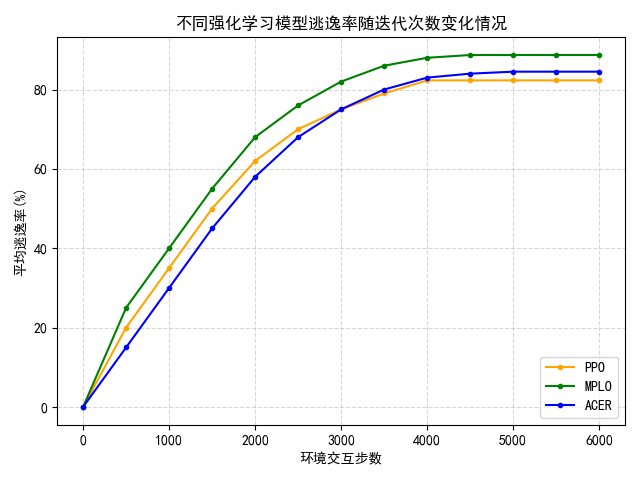
\includegraphics[width=0.75\textwidth]{figures/5.1}
	% \caption[这里的文字将会显示在 listoffigure 中]{这里的文字将会显示在正文中}
	\caption{不同强化学习模型性能训练对比图}\label{fig:5.1}
\end{figure}

其次,MPLO 在修改代价方面同样具有竞争力。它的平均扰动数为3.8次,仅略高于PPO的3.2次,显著低于ACER的4.1次。这表明,在生成同等数量的对抗样本时,MPLO 能以更少的操作步骤完成目标,减少了对原始文件结构的破坏,提高了生成对抗样本的隐蔽性和功能保留度。

In the modification cost aspect, MPLO are also comparative. Its average perturbation time is 3.8, slightly higher than 3.2 of PPO, extremely lower than 4.1 of ACER, indicating that MPLO can complete the goal with lower operation steps at the premise that different models generate same amount adversarial samples, reducing original file structure disruption, improving the generated samples' concealment and functional retention.

最后,从收敛速度来看,MPLO在4500步时就已实现策略稳定,虽然略慢于PPO(4200步),但明显快于ACER(5000步)。这一表现反映了MPLO 在策略更新和经验利用上的高效平衡:通过多维度策略评估机制,它能在探索和利用之间保持良好节奏,快速逼近最优扰动策略,而无需进行过度的样本回放或过长的训练迭代。

Considering the convergence speed, MPLO achieves policy convergence at 4,500 steps, slower than 4,200 steps of PPO but faster than 5,000 steps of ACER, reflecting that MPLO gets an effective balance between exploration and exploitation. Through multi-dimensional strategy evaluation mechanisms, it can maintain the balance between exploration and exploitation, rapidly approaching optimal disturbance strategies without requiring excess sample replay and exceeding training iterations.

\begin{table}[htbp]
	\centering
	\caption{强化学习模型性能对比}
	\label{tab:5.9}
	\begin{tabular*}{0.9\textwidth}{@{\extracolsep{\fill}}cccc}
		\toprule
		模型 & 平均逃逸率(\%) & 平均扰动数(次) & 收敛速度(环境交互步数) \\
		\midrule
		PPO & 82.3 & 3.2 & 4200 \\
		MPLO & 88.7 & 3.8 & 4500 \\
		ACER & 84.5 & 4.1 & 5000 \\
		\bottomrule
	\end{tabular*}
\end{table}

为了更全面地验证本文提出的对抗性样本生成方法(MPLO)方法在对抗样本生成方面的有效性,本文选取MalConv\cite{raff2017malware}作为目标检测模型,在与其他强化学习方法相同的实验环境下,对比分析两者在逃逸攻击场景中的表现。对比实验遵循统一的设置标准,采用相同的1000个恶意ELF文件作为攻击目标,最大修改步数限制为20步,以保证实验的公平性和可比性。

To comprehensively certify MPLO's effectiveness in adversarial sample generation, this research selects MalConv\cite{raff2017malware} as the target detection model, analyzing its evasion attack performance and the other RL model's performance in the same experiment environment. The comparative experiment follows the unified setting standard, adopting 1,000 malicious ELF files as the attack target and restraining the maximum modification step to 20 to ensure the fairness and comparability of the experiments.

与基于深度强化学习的对抗样本生成方法不同,本文所提出的MPLO方法具有无需大量训练、生成效率更高的特点。在有限修改范围内快速生成高效扰动样本,以提高逃逸成功率的同时尽量减少对原始样本的结构性破坏,保证对抗样本的隐蔽性和实用性。设定baseline为孙贺\cite{孙贺2024基于深度强化学习的恶意}等人提出的基于深度强化学习的对抗样本生成方法,使用结构扰动扰动样本,DP-GAN\cite{zhan2024enhancing}为一种基于强化学习的对抗性恶意软件生成框架,创新性地引入了内在好奇心奖励模块(ICM)来解决黑盒场景下奖励稀疏的问题,并利用生成对抗网络(GAN)生成合成字节作为动作内容。

Unlike adversarial sample generation methods based on deep RL, the MPLO method proposed by this research exhibits no reliance on numerous training and high generating efficiency characteristics, swiftly generating perturbated samples with high efficiency in limited modification area, lessening structural disruption to original samples while improving evasion rate, and maintaining adversarial samples' concealment and practicality. The baseline method uses an adversarial sample generation method based on deep RL, proposed by Sun et al\cite{孙贺2024基于深度强化学习的恶意}. Using samples with structural disturbance, DP-GAN\cite{zhan2024enhancing}, a framework based on RL incorporating an Intrinsic Curiosity Module (ICM) is introduced for solving sparse rewards problems in the black-box scenario and generating synthetic bytes by utilizing generated adversarial network as action contents.

为全面评估性能,本文分别从逃逸成功率(即生成的对抗样本能够成功绕过目标检测器的比例)、平均修改步数(每个成功样本平均修改字节数)以及平均生成时间(每个样本生成所需时间)三项关键指标进行定量对比分析。实验结果如表\ref{tab:5.10}所示。

To evaluate the performance comprehensively, this research conducts quantitative comparative analysis on evasion success rate (the rate of generated adversarial samples that can successfully evade the detection of the target detector), average modification times (the average bytes modified in each successful sample) and average generating time (the time required for each sample generation) respectively. The results are illustrated in Table \ref{tab:5.10}.

\begin{table}[htbp]
	\centering
	\caption{逃逸主流检测模型性能对比}
	\label{tab:5.10}
	\begin{tabular*}{0.9\textwidth}{@{\extracolsep{\fill}}cccc}
		\toprule
		模型 & 平均逃逸率(\%) & 平均修改步数(次) & 平均生成时间(ms) \\
		\midrule
		Baseline & 48.20 & 5.4 & 212 \\
		MPLO & 71.25 & 4.7 & 186 \\
		DP-GAN & 67.70 & -- & -- \\
		\bottomrule
	\end{tabular*}
\end{table}

在对比MPLO与DP-GAN模型时,MPLO展现出了明显的优势。首先,MPLO的平均逃逸率为71.25\%,明显高于DP-GAN的67.70\%,显示出MPLO在生成对抗样本时的更高成功率。

The comparison between MPLO and DP-GAN shows that MPLO exhibits an obvious advantage. The average evasion rate of MPLO is 71.25\%, which is significantly higher than DP-GAN's 67.70\%, represents that MPLO has a higher success rate in adversarial sample generation.

与此同时,MPLO 的平均修改步数降至4.7次(Baseline为5.4次,说明其扰动更加紧凑,能够以更少的操作步骤实现逃逸,从而更好地保留原始样本的语义和功能。

Meanwhile, the average modification times of MPLO decreases to 4.7, which is lower than Baseline's 5.4, indicating that its perturbations are more compact, achieving evasion in less operation steps, thus retaining original sample's semantics and functionality more effectively.

在生成效率方面,MPLO 方法的平均生成时间为186ms,相比Baseline的212ms 缩短了约12\%。这一性能提升进一步验证了MPLO在大规模样本处理和高频逃逸需求场景下具有更好的实用性与部署优势。

In the evaluation of generation efficiency, the average generation time of MPLO is 186ms, 12\% faster than Baseline's 212ms. This performance development further verifies that MPLO exhibits higher practicality and deployment advantages in scenarios with large-scale samples and high evasion requirements.

为全面评估所提出对抗样本生成框架在真实运行环境中的动态逃避检测能力,本文进一步将部分生成的对抗样本上传至腾讯哈勃(Tencent Habo)动态分析平台进行行为检测测试。腾讯哈勃是当前广泛应用的沙箱分析平台之一,具备多引擎动态检测能力,能够在模拟的真实系统中运行样本并监测其文件操作、进程调用、注册表修改、网络连接等可疑行为特征。

To evaluate the dynamic evasion capability in real environments of the adversarial sample generation framework proposed in this research, this research uploads parts of generated samples to Tencent Habo dynamic analysis platform to conduct behavioral analysis detection. Tencent Habo is one of the sandbox analysis platforms that is widely used with multiple engines dynamic detection. It can simulate executing samples in real systems and record suspicious behavioral features, such as file operations, process calls, registry modifications and network connections.

在实验中,选取Doss木马典型样本作为代表。样本上传至腾讯哈勃后,平台返回检测评分和行为标签。结果显示,经过本文对抗策略处理后的样本整体检测结果从恶意转变为了未知。

In this research, DDoS Trojan samples are selected as representatives. The platform returns detection scores and behavioral labels after the samples are uploaded to Tencent Habo. The result demonstrates that the results of samples processed by adversarial strategies changes from malicious to unknown.

\begin{figure}[hbt]
	\centering
	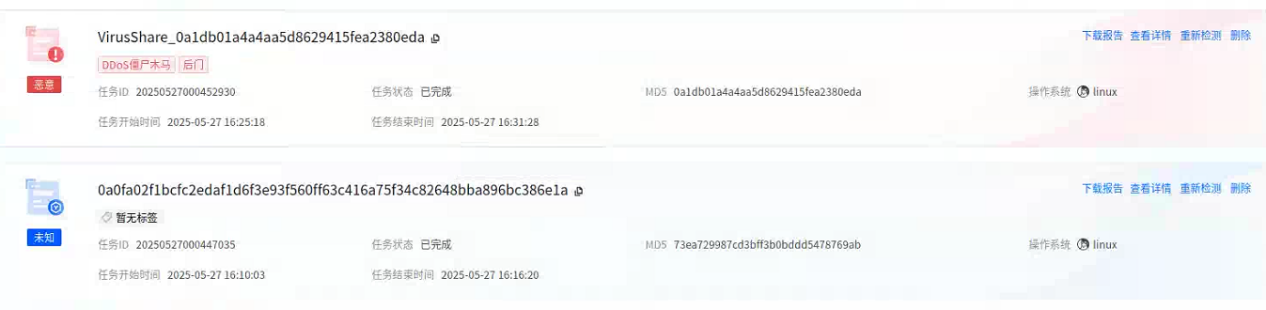
\includegraphics[width=0.75\textwidth]{figures/5.2}
	% \caption[这里的文字将会显示在 listoffigure 中]{这里的文字将会显示在正文中}
	\caption{免杀前后哈勃检测结果对比}\label{fig:5.2}
\end{figure}

此外,动态行为日志也显示,对抗样本在运行时触发的可疑行为数量明显减少,如“远程线程注入”、“可疑网络通信”、“内存Shellcode行为”等关键行为均未被触发或未达检测阈值。这说明所生成样本不仅在静态特征层面成功规避了特征匹配类检测系统,同时在动态行为层面也具备较强的对抗能力。

Besides, suspicious behaviors (e.g., remote thread injections, suspicious network communications, memory shellcode execution) were significantly reduced or undetected.
This confirms that generated samples evade both static feature matching and dynamic behavioral analysis.

综上所述,腾讯哈勃动态检测实验进一步验证了本文所提出的多维扰动策略在真实沙箱环境中的隐蔽性与有效性,从而佐证该框架具备较强的实用潜力与安全研究价值。

In summary, Tencent Harbo dynamic detection experiment further validates the concealment and validity of multi-disturbance strategies issued in this research, proving that this framework is practically potential and exhibits high research value. 

\section{对抗样本生成方法的消融实验 Ablation Experiments on Adversarial Sample Generation Methods}

为了评估本文提出的多架构对抗性样本生成的必要性,计划实验测试结构扰动、指令扰动和行为扰动在逃避恶意软件检测中的独立效果,本文设计了消融实验,逐一去除不同的扰动方法,并分析其对检测系统逃避能力的影响。

To evaluate the necessity of the multi-dimensional adversarial sample generation approach proposed in this research, ablation experiments were designed to test the individual effects of structural, instructional, and behavioral perturbations in the evading malware detection aspect. Each disturbance method was systematically ablated by removing it, allowing analyzing its impact on detection evasion capabilities.

在本实验中,使用了本文收集的恶意软件样本的标准数据集,从中随机挑选1000个样本,并应用以下三种扰动方法对样本进行单独扰动,来查看对本文训练的随机森林检测算法的性能。通过与基准组(本研究方法)进行对比,研究者可以系统地评估每种扰动策略对恶意软件检测逃避能力的影响。

In this experiment, 1,000 randomly selected samples from the malware dataset were perturbed individually using three distinct methods, evaluating performance against the random forest detector trained in this study. Comparison with the baseline group allowed researchers to systematically assess each perturbation's contribution to evasion.

实验组1:结构扰动

Experimental Group 1: Structural Perturbation

在这一实验组中,本文采用结构扰动方法,主要通过修改恶意样本的程序结构(如修改段表、修改符号表、重新排列代码段等)来扰乱程序的结构信息。此扰动方法的目标是通过破坏程序的结构信息,使得静态分析工具无法准确地识别恶意行为。

This group adopted structural perturbations by modifying program structures of malware samples (e.g., altering section tables, symbol tables, or rearranging code segments). This method's target is disrupting structural information, preventing static analysis tools from accurately identifying malicious behaviors.

实验组2:指令扰动

Experimental Group 2: Instructional Perturbation

该组实验单独应用指令扰动技术,通过对恶意样本中的指令进行修改、重排或替换,从而改变程序的指令序列。例如,使用等价指令替换原有的指令,或者调整指令执行顺序,确保程序逻辑不变的同时有效干扰指令级别的分析。

This group solely employed instructional perturbations by modifying, reordering, or replacing instructions in malware samples. Modification examples include replacing instructions with functional equivalents or rearranging execution sequences while preserving program logic unchanged to evade analysis at the instruction level.

实验组3:行为扰动

Experimental Group 3: Behavioral Perturbation

本组实验使用行为扰动,行为扰动方法主要通过修改恶意样本的行为逻辑,使其在特定环境下不表现出原本的恶意行为。常见的行为扰动包括通过引入时间延迟、控制流混淆等手段使恶意行为的触发条件延后或改变,从而规避动态行为分析的检测。

This group exclusively implemented behavioral perturbations through altering malicious behavioral logic. Common techniques included inserting time delays or control-flow obfuscation to delay or modify malicious behavior triggers, thus evading dynamic behavioral analysis.

实验组4:基准组

Experimental Group 4: Baseline Group

该组实验使用本文所示的多架构扰动方法扰动,联合使用结构扰动、指令扰动、行为扰动三种扰动。

This group applied the proposed multi-dimensional perturbation method, jointly employing structural, instructional, and behavioral perturbations.

实验结果如表\ref{tab:5.11}所示。

Experimental results are descirbed in Table \ref{tab:5.11}.

\begin{table}[htbp]
	\centering
	\caption{消融实验性能对比}
	\label{tab:5.11}
	\begin{tabular*}{0.9\textwidth}{@{\extracolsep{\fill}}ccc}
		\toprule
		扰动方式 & 平均逃逸率(\%) & 平均生成时间(ms) \\
		\midrule
		结构扰动 & 72.5 & 156 \\
		指令扰动 & 52.6 & 218 \\
		行为扰动 & 12.1 & 175 \\
		MPLO(多策略组合) & 87.2 & 183 \\
		\bottomrule
	\end{tabular*}
\end{table}

实验结果显示,不同扰动策略在逃避恶意软件检测方面表现出明显差异。结构扰动通过修改段表、符号表等程序结构信息,在静态分析阶段表现出较强的对抗能力,平均逃逸率达到72.5\%。这说明此类扰动能够有效破坏传统静态特征提取过程,提升样本的不可识别性。然而,结构扰动对动态分析影响有限,因为行为逻辑未发生本质变化,样本在实际运行中仍可能被行为分析引擎识别。

Structural perturbations are achieved by modifying program structures such as section tables and symbol tables, exhibiting strong adversarial capabilities during static analysis. The average evasion rate of structural perturbations is 72.5\%. This indicates effective disruption of traditional static feature extraction processes, enhancing sample obfuscation. However, structural perturbation is limited to affect dynamic analysis since behavioral logic remains fundamentally unchanged. The samples may still be detected by analysis engines during real execution processes.

指令扰动策略以等价指令替换、指令重排等方式改变指令序列,从而混淆基于指令特征的静态检测模型。虽然其逃逸率为52.6\%,显著低于结构扰动,但仍能在一定程度上规避静态签名匹配。值得注意的是,此类扰动并未改变程序行为,故在基于行为分析的检测系统下几乎无额外收益。此外,其生成时间相对较长(218ms),反映出操作粒度较高带来的计算开销。

Instructional perturbations are implemented through equivalent instruction substitution and instruction resorting and achieve a 52.6\% evasion rate. Although the evasion rate of instructional perturbations is significantly lower than structural perturbations, instruction perturbations still are effective against static signature matching. What should be paid more attention to is that this approach doesn't alter program behavior, yielding minimal additional benefits against behavioral analysis. Otherwise, its generation time (218ms) reflects higher computational resource consumption in higher granular operations.

行为扰动则主要通过引入延时逻辑、控制流调整等方式,推迟或隐藏样本的恶意行为触发条件,从而干扰沙箱等动态分析环境的行为提取过程。虽然行为扰动理论上应有助于绕过动态检测,但在本实验中仅取得12.1\%的逃逸率,说明此类扰动在扰动静态分析模型上的性能并不明显。

Behavioral perturbation employs techniques like delayed triggers and control flow adjustments to postpone or hide malicious actions trigger conditions, thus interfering with dynamic analysis environments like sandboxes. Despite theoretical effectiveness against dynamic detection, it achieves only 12.1\% evasion rate. The low evasion rate demonstrates this model's limited impact on static analysis models.

相比上述三种单一扰动策略,MPLO综合引入结构、指令与行为扰动机制,获得了最高的逃逸率87.2\%,远超所有单一扰动策略,且生成时间控制在183ms,显示出良好的攻击效果与生成效率平衡。这表明,多维度扰动策略间具有显著的互补性:结构扰动提供静态特征级混淆,指令扰动增强细粒度隐藏能力,而行为扰动则补充动态逃逸能力。联合使用可突破各类检测模型的多重防线,实现更具普适性和稳定性的对抗样本生成。

Comparison with three single disturbance strategies, MPLO comprehensively introduces structural, instructional, and behavioral perturbation mechanisms, achieves the highest evasion rate (87.2\%) and limits the generation time in 183ms. This result exhibits complementary advantages: structural perturbation confuses static features, instructional perturbation enhances fine-grained stealth, and behavioral perturbation enables dynamic evasion. Combining these strategies, it bypasses multi-layered detection defenses for more robust adversarial sample generation with higher adaptivity and stability.

综上所述,消融实验验证了MPLO方法中各扰动策略的独立作用和协同价值。结果表明,单一扰动策略虽具备一定逃逸能力,但难以在面对多类型检测模型时保持稳定表现。而将多种扰动策略集成在统一框架中,不仅能提升整体逃逸率,也有助于在实际攻防场景中实现更强鲁棒性与可操作性。

The ablation study confirms both independent and synergistic value of each perturbation strategy in MPLO. Individual strategies show partial evasion capabilities but cannot keep stable while facing multiple detection models.Integrating perturbation strategies in a unified framework significantly enhances overall evasion performance, practical applicability, and robustness against diverse detection models.  

\section{功能保留研究 Research on Functional Retention}

在对抗性恶意样本生成任务中,保持扰动后的样本依然具备原始功能,是衡量样本有效性和实用价值的重要标准。若样本虽能逃避检测,却失去了原本的恶意行为功能,则其在真实攻击模拟、安全评估及系统对抗训练中的价值将大打折扣。因此,本文对提出的三类扰动方法——结构扰动、指令扰动与行为扰动——分别开展功能保留性研究,系统评估每类扰动对恶意功能完整性的影响。

In adversarial malware sample generation tasks, preserving the original functionality of perturbed samples serves as a critical criterion for evaluating their effectiveness and practical values. Samples that evade detection but lose their malicious functionality diminish their value in real attack scenario simulations, security assessments, and system defense training. Therefore, this study systematically conducts the research on the malicious functionality impact of the three proposed perturbation methods—structural, instructional and behavioral.

(1)结构扰动的功能保留性分析

(1) Functional Preservation Analysis of Structural Perturbation

结构扰动主要作用于程序的元数据与文件结构层面,如段表重排、符号表修改、节区添加与重命名等。这类扰动并不改变程序的指令逻辑或运行流程,因此在理论上不会影响样本的实际执行功能。

Structural perturbation primarily modifies metadata and file structures of programs, such as section table rearrangement, symbol table modification, section addition and section renaming. Such disturbances do not alter the program's instruction logic or execution flow, theoretically maintaining its functional behavior.

在实验中,本文对数百个经过结构扰动处理的恶意样本在受控沙箱中进行自动执行,观测其关键行为特征(如反连行为、键盘监听、文件篡改等)。结果表明,绝大多数结构扰动样本在执行过程中表现出与原样本高度一致的行为特征,功能保留率(Functionality Retention Rate, FRR)达到92.4\%。个别失效样本主要由于过度扰动了加载器相关节区或破坏了符号重定位信息所致,可通过更精细的扰动控制予以修复。

Hundreds of structurally perturbed malware samples were executed in the controlled sandbox to observe their crucial behavioral characteristics (e.g., reverse connections, keystroke logging, and file tampering). The results show that most structurally perturbated samples represent highly identical to the original samples. The functionality retention rate reached 92.4\%. The failure samples are mainly caused by disturbing excessively on sections of the loader or disrupting symbol relocation information. These conditions can be fixed by adopting more intricate disturbance controls.

(2)指令扰动的功能保留性分析

(2) Functional Preservation Analysis of Instructional Perturbation

指令扰动旨在修改程序代码本体,包括等价指令替换、指令重排、插入无操作指令(NOP)、使用跳转替换顺序结构等。该类扰动技术高度依赖语义保持(semantic-preserving)原则,其核心在于不改变程序逻辑的同时最大限度混淆静态指令序列。

Instructional perturbations aim to modify program code, including equivalent replacement of sequential structures with jumps. These techniques highly depend on following semantic-preserving principles to obfuscate static instruction sequences without altering program logic.

利用控制流完整性(CFI)检查、执行路径比对等方式评估指令扰动的功能影响。实验结果显示,96\%以上的样本在扰动后依旧可以正常运行,并实现原始恶意行为,如建立远程通信、窃取数据等。功能保留率达到93.7\%。少数失败样本主要源于对跳转逻辑、栈平衡或调用约定的破坏,提示未来在扰动生成过程中应引入更严格的约束机制,以确保扰动的语义一致性。

Utilizing Control Flow Integrity (CFI) checks and execution path comparison methods, experimental results demonstrate that more than 96\% of samples maintained original malicious behaviors (e.g., establishing remote communication, data exfiltration) after perturbations and the FRR reached 93.7\%. Minor failure samples occurred due to disrupted jump logic, stack imbalance, or calling convention violations, which suggests that future implementations should incorporate stricter constraints for semantic consistency.

(3)行为扰动的功能保留性分析

(3) Functional Preservation Analysis of Behavioral Perturbation

行为扰动通过延迟恶意行为的触发、插入混淆控制流、依赖特定条件执行等方式干扰行为分析工具的检测窗口。这种策略改变的是恶意行为的触发机制而非其具体逻辑,因此其功能保留性具有一定的条件性。

Behavioral perturbations interfere with behavioral analysis tools by delaying malicious behavior triggers, inserting obfuscated control flows, and introducing conditional execution dependencies. This strategy alters the triggering mechanism rather than the core malicious logic, resulting in conditional functionality preservation.

在实验中,本文对扰动后的样本进行加长执行时间操作,验证其是否仍能触发原始恶意行为。结果显示,98\%的行为扰动样本能够在设置合理触发条件后完全复现原始恶意行为。

In this research, prolonging disturbed samples' execution time verifies whether the original malicious behaviors can be triggered. The results show that 98\% of behaviorally perturbed samples fully replicated original malicious behaviors under appropriately configured trigger conditions.

为全面对比三类扰动的功能保留效果,本文统计了每类扰动样本的成功执行率及功能保留率,结果如下表\ref{tab:5.12}所示。

To comprehensively compare functional retention results of three perturbation strategies, this research compile statistics on each sample's success execution rate and functional retention rate. The results are provided in Table \ref{tab:5.12}.

\begin{table}[htb]
	\centering
	\caption{功能保留研究结果}
	\label{tab:5.12}
	\begin{tabular*}{0.9\textwidth}{@{\extracolsep{\fill}}ccc}
		\toprule
		扰动类型 & 成功执行率(\%) & 功能保留率(\%) \\
		\midrule
		结构扰动 & 99.2 & 92.4 \\
		指令扰动 & 96.5 & 93.7 \\
		行为扰动 & 82.7 & 98.0 \\
		\bottomrule
	\end{tabular*}
\end{table}

从结果可以看出,结构扰动在不破坏程序逻辑的前提下具有很好的功能保留性;指令扰动在合理控制下也能维持较高功能一致性;行为扰动由于引入了复杂触发机制,成功率有所下降,但功能保留性最高。

All in all, structural perturbation maintains high functionality retention without disrupting program logic. Instructional perturbation achieves strong consistency under controlled constraints. Behavioral perturbation, despite lower execution success rates due to complex triggering mechanisms, exhibits the highest functionality retention capability.

\section{样本迁移性研究 Research on Sample Transferability}

为了进一步验证本文所提出的多架构对抗样本生成方法在真实检测环境中的有效性,本文开展了样本迁移性研究,将生成的对抗样本上传至公共在线恶意软件检测平台VirusTotal,评估其在不同商用反病毒引擎下的实际逃避能力。该实验旨在考察对抗样本从本地检测系统向多引擎平台的迁移能力,即:在本地检测模型中成功逃避的样本是否同样能够在第三方检测平台中保持对抗性。

To further validate the effectiveness of the proposed multi-architecture adversarial sample generation method in real detection environments, this research evaluates sample transferability. Adversarial samples were submitted to the public online malware detection platform VirusTotal to analyze their practical evasion capabilities among different commercial antivirus engines. This experiment examines whether samples that successfully evade the local detection model can retain adversarial properties on the third-party detection platforms.

本实验从经过结构扰动、指令扰动和行为扰动处理的对抗样本中,分别选取代表性样本进行测试,并与未扰动的原始恶意样本进行对比。所有样本均上传至 VirusTotal 平台进行静态和动态联合扫描,记录各引擎的检测结果,统计每个样本的被检测引擎数量(即“命中率”),作为衡量迁移逃避能力的标准。

This research selects representative samples from adversarial samples modified by structural perturbations, instructional perturbations, and behavioral perturbations, and compares them with original malicious samples without modification. All samples were uploaded to VirusTotal for static and dynamic scanning. Detection results from each engine were recorded. The number of engines detecting each sample (i.e., "hit rate") was collected as the metric for evasion capability.

\begin{figure}[htbp]
	\centering
	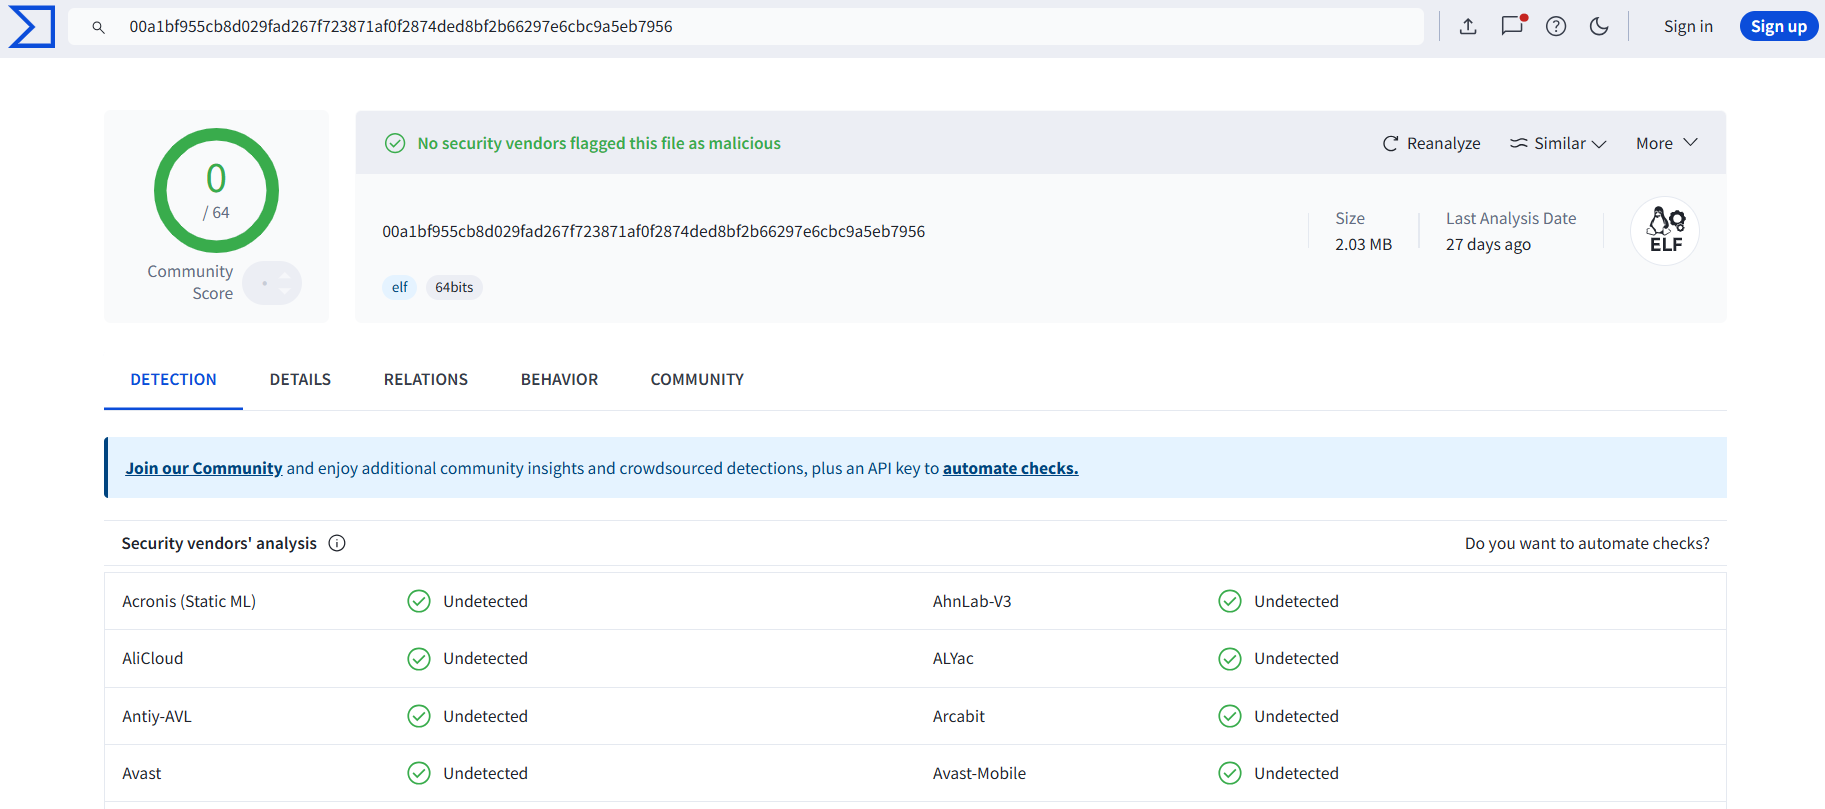
\includegraphics[width=0.75\textwidth]{figures/5.3}
	% \caption[这里的文字将会显示在 listoffigure 中]{这里的文字将会显示在正文中}
	\caption{经对抗性学习后VirusTotal扫描结果}\label{fig:5.3}
\end{figure}


为更好地展示免杀效果,此处定义Virustotal检测率$v_t$为可检测到样本恶意性的杀毒引擎数占总杀毒引擎数之比,如下计算: 

To better illustrate the evasion effect, the VirusTotal detection rate $v_t$ is defined as the ratio of antivirus engines detecting maliciousness to the total number of engines, calculated as the formulation below:
\begin{equation}
v_t = \frac{D_e}{A_e}
\tag{5.9}
\end{equation}

其中$D_e$为可检测到样本恶意性的杀毒引擎数,$A_e$为总杀毒引擎数。

$D_e$ is the number of antivirus engines detecting maliciousness, while $A_e$ presents the total number of antivirus engines.

表\ref{tab:5.13}列举了20个样本在VirusToal网站上免杀前检测率$v_{t1}$、免杀后检测率$v_{t2}$以及下降率$vt_{down}$。

Table \ref{tab:5.13} lists the detection rates $v_{t1}$ before evasion, $v_{t2}$ after evasion, and the decline rate $vt_{down}$ of20 samples on VirusTotal.

\begin{table}[htbp]
	\centering
	\caption{经免杀后VirusToal扫描结果前后对比}
	\label{tab:5.13}
	\begin{tabular*}{0.9\textwidth}{@{\extracolsep{\fill}}cccc}
		\toprule
		名称 & 免杀前检测率 & 免杀后检测率 & 下降率 \\
		\midrule
		e601de9bb0828bae5eec828547d18e84 & 39/62 & 2/62 & 94.87\% \\
		e61865927c25a33f57b3385f59d45bf8 & 40/59 & 3/62 & 92.5\% \\
		e62288919ce96bbe2d382c49797d5e99 & 41/62 & 5/62 & 87.8\% \\
		e6344bb726c1b97e277c478bb7a2ddab & 32/61 & 3/60 & 90.62\% \\
		e6450e7a705060df1795b18bc853416d & 40/62 & 2/62 & 95.0\% \\
		e64e06c16591f46ec8759be807f7b34c & 38/62 & 0/62 & 100.00\% \\
		e69ba88b83c142b2f04f857787fdfb5e & 38/62 & 3/62 & 92.11\% \\
		e6df850bfa010aa039511504ccd917db & 37/62 & 5/62 & 86.49\% \\
		e6e6891c01c56533919a3f9f677f6467 & 41/62 & 2/62 & 95.12\% \\
		026f98e26942d5745b589069cf6dd143 & 41/62 & 3/62 & 92.68\% \\
		e704b5769c02ff5ccc7f53ca46d63fd2 & 43/61 & 4/62 & 90.70\% \\
		e711723f3301251615d6009382c7234b & 43/62 & 3/62 & 93.02\% \\
		056e32863c0483922464fee50b2bbd37 & 39/62 & 2/62 & 94.87\% \\
		031be2bf69f1fbe13d78c2ac93508753 & 41/62 & 3/62 & 92.68\% \\
		e789b8bb45c88a64f682fb434eb50bcc & 38/62 & 2/62 & 94.74\% \\
		e9ea5cbcba4f9406f9926ff0080997a3 & 42/62 & 5/62 & 88.10\% \\
		e9ee698553866065fa6bdb0764df2564 & 37/62 & 4/62 & 89.19\% \\
		eacd3c9972ab6c22267d3eda9addf9a6 & 40/61 & 0/62 & 100.00\% \\
		032de9e9ee32b91053b8195422fb2133 & 41/62 & 3/62 & 92.68\% \\
		eaf1a8c6eb5fa1641517de35fefb1a18 & 36/63 & 5/62 & 86.11\% \\
		\bottomrule
	\end{tabular*}
\end{table}

\begin{table}[htbp]
	\centering
	\caption{本文方法与现有工作的对比分析}
	\label{tab:5.14}
	\begin{tabular*}{\textwidth}{@{\extracolsep{\fill}}ccccc}
		\toprule
		工作 & 病毒类型 & 攻击方式 & 评估的检测模型数量 & 平均免杀率 \\
		\midrule
		{[22]} & PE 病毒 & 黑盒攻击 & 1 & 60.0\%(MalConv 网络) \\
		{[68]} & Android 病毒 & 白盒攻击 & 10 & 59.37\%(平均) \\
		{[69]} & PE 病毒 & 黑盒攻击 & 3 & 70.0\%(商用 AV) \\
		{[26]} & PE 病毒 & 黑盒攻击 & 5 & 74.4\%(EMBER 模型) \\
		{[70]} & ELF 病毒 & 黑盒攻击 & 64 & 75.8\%(VirusTotal) \\
		本文 & ELF 病毒 & 白盒攻击 & 62 & 84.5\%(VirusTotal) \\
		\bottomrule
	\end{tabular*}
\end{table}

实验结果表明,经过扰动处理的对抗样本在 VirusTotal 平台上的总体检测率相比原始样本显著降低,表现出较强的迁移性。其中,结构扰动样本的逃避能力最为稳定,多个依赖静态分析特征的引擎未能识别其恶意特征;指令扰动样本在部分引擎中表现出一定逃避效果,但整体变异幅度相对较小;行为扰动样本在动态检测能力较弱的引擎中效果较好,但在支持沙箱分析的引擎中仍存在部分命中情况,说明其对动态特征的干扰存在一定的平台依赖性。

Experimental results indicate that adversarial samples processed by perturbation exhibit extremely lower overall detection rates on VirusTotal than original samples, exhibiting strong transferability. Structural perturbations achieved the most stable evasion, with multiple static analysis-dependent engines failing to identify malicious features. Instructional perturbations showed limited evasion across engines, yielding relatively overall smaller variations. Behavioral perturbations effectively evaded engines with weaker dynamic detection capabilities, but there still exist partial detections in engines supporting sandbox analysis. The limitation shows platform-specific dependencies in dynamic feature interference.

此外,不同扰动方式对引擎类型的影响也存在差异。结构扰动主要干扰依赖程序结构解析和静态特征提取的引擎,指令扰动则影响基于指令签名和机器学习模型的检测器,行为扰动更容易绕过基于沙箱执行路径和行为模式的动态检测机制。该实验结果进一步验证了对抗扰动在多引擎、跨平台检测环境下的适应性与实际应用价值。

Furthermore, different perturbation methods affected engine types distinctly. Structural perturbation primarily disrupted engines relying on static structure parsing and feature extraction. Instructional perturbation impacted detectors based on instructional signatures or machine learning models. Behavioral perturbation more readily evaded dynamic mechanisms based on sandbox execution paths and behavioral patterns. These results further validate the adaptability and practical utility of adversarial perturbations in multi-engine, cross-platform detection environments.

本文生成的对抗样本不仅能够在本地检测模型中实现有效规避,同时也能在真实检测平台中表现出良好的迁移能力,具备较强的跨平台逃逸效果,为对抗性恶意软件研究和实战应用提供了有力支撑。

The adversarial samples generated in this research not only achieve effective evasion in local detection models but also demonstrate strong transferability in real detection platforms, exhibiting robust cross-platform escape effects. This provides solid support for adversarial malware research and practical applications.

为了更系统地分析本文方法与现有研究之间的差异与优势,表\ref{tab:5.14}从多个角度对比了当前典型对抗性恶意样本生成工作与本研究的技术特征和实验效果,涵盖了病毒类型、攻击方式、检测模型数量以及平均免杀率四个关键维度,定性与定量地展示了本文工作的综合性能。

To systematically analyze the differences and advantages between the proposed method in this experiment and existing research, Table \ref{tab:5.14} compares current typical adversarial malware sample generation works with this research across four key dimensions: virus types, attack methods, number of detection models, and average evasion rate. This table qualitatively and quantitatively describes the comprehensive performance of this work.

在病毒类型方面,已有多数研究主要聚焦于 Windows 平台下的 PE 病毒或移动平台上的 Android 病毒,对 Linux 平台 ELF 格式恶意代码的研究相对稀缺。相比之下,本文专注于 ELF 病毒的对抗样本生成与逃逸效果评估,有效填补了该领域的研究空白。

In the virus type aspect, most existing studies concentrate primarily on PE viruses in Windows platforms or Android viruses in mobile platforms, with relatively scarce research on in the ELF format malware in Linux platforms. In contrast, this study focuses on adversarial sample generation and escape effect evaluation for ELF virus realm. This research effectively fills this research gap of ELF adversarial malware generation.

在攻击方式方面,本文所提出的方法与文献\cite{rathore2021identification}属于白盒攻击方式,需了解检测模型的特征提取方式和训练数据分布等内部信息。而文献\cite{kolosnjaji2018adversarial,quertier2022merlin,song2022mab} 类似,均采用黑盒攻击模式,无需依赖检测模型的内部结构,仅通过输入输出结果进行扰动优化。

Comparing attack methods, the approach issued in this paper belongs to the white-box attack category, like the method in literature \cite{rathore2021identification}. The white-box attack requires knowledge of internal information such as the feature extraction methods and training data distribution of the detection model. Different from this research, some literatures \cite{kolosnjaji2018adversarial,quertier2022merlin,song2022mab} employs a black-box attack pattern. Unlike white-box attack, black-box attack eliminates dependency on the internal structure of detection models and optimizes disturbances solely through input and output results.

相比之下,另一项基于强化学习的自动生成 ELF 对抗恶意样本的方法\cite{xue2024reinforcement},结合了多轮特征提取、恶意检测与智能决策的闭环机制,利用 PPO 算法在 Linux x86 平台实现了对 ELF 恶意样本的有效扰动与免杀。

In Comparison, another method for automatically generating ELF adversarial malware samples based on RL\cite{xue2024reinforcement} incorporates a multi-loop mechanism combining multi-round feature extraction, malware detection, and intelligent decision-making. Utilizing the PPO algorithm, it achieves effective perturbation and evasion of ELF malware samples on the Linux x86 platform.

虽然该方法与本文均采用强化学习框架,但本文更侧重于多维度的大规模评估,覆盖62个检测引擎,强调了方法的广泛适用性和鲁棒性;同时本文在动作空间设计、特征选择及攻击策略上进行了改进,实现了更高的平均免杀率,体现了方法在实际应用中的竞争优势。

Although both this method and the method issued in research adopts reinforcement learning frameworks, the present work focuses more on multidimensional large-scale evaluation, covering 62 detection engines to emphasize broad applicability and robustness. Simultaneously, improvements in action space design, feature selection, and attack strategies have been updated. This innovation results in a higher average evasion rate and reflects the competitive advantage of the approach in practical applications.

在平均免杀率方面,本文所生成的对抗样本在 VirusTotal 平台中取得了 84.5\% 的免杀率,优于其他研究的平均水平。这表明本文提出的对抗扰动策略在逃逸检测方面具有更强的效果。

In terms of average evasion rate, the adversarial samples generated in this research achieved 84.5\% evasion rate on the VirusTotal platform, surpassing the average levels reported in other studies. This indicates that the proposed adversarial perturbation strategy demonstrates stronger effectiveness in evading detection.

\section{本章小结}

本章在统一的软硬件与数据集条件下,先对PPO、ACER及Baseline方法与所提出的多维度策略优化模型(MPLO)在不同LSTM层数与隐藏层规模配置下的逃逸成功率、扰动次数和收敛速度进行了深入对比,继而通过消融实验评估了结构扰动、指令扰动与行为扰动三种策略的独立效果及其组合增益,并结合沙箱执行与控制流完整性检测检验了各类扰动对恶意功能保留的影响;最后,将生成的对抗样本上传至VirusTotal平台,对比了免杀前后检测率及下降幅度,以全面验证模型在跨引擎环境中的迁移逃逸能力。实验结果显示,MPLO 表现出更高的攻击成功率、更低的扰动成本、更快的收敛速度及更强的跨平台迁移性能。




\backmatter

% 结论
%%
% The BIThesis Template for Graduate Thesis
%
% Copyright 2020-2023 Yang Yating, BITNP
%
% This work may be distributed and/or modified under the
% conditions of the LaTeX Project Public License, either version 1.3
% of this license or (at your option) any later version.
% The latest version of this license is in
%   https://www.latex-project.org/lppl.txt
% and version 1.3 or later is part of all distributions of LaTeX
% version 2005/12/01 or later.
%
% This work has the LPPL maintenance status `maintained'.
%
% The Current Maintainer of this work is Feng Kaiyu.

\begin{conclusion}

本文提出了一种基于强化学习的多维度对抗性恶意软件生成框架,旨在有效应对日益复杂的恶意软件检测挑战。该框架通过在结构层、指令层及行为层对恶意样本进行扰动,并引入良性样本字节作为扰动来源,从多个维度提升了对抗样本的隐蔽性与逃避检测能力。具体而言,本文的主要创新点和工作如下:

This paper proposes a multi-dimensional adversarial malware generation framework based on RL to effectively address increasingly complex malware detection challenges. The framework aims to perturbate malware at the structural later, instruction layer, and behavioral layer, and introduces bytes from benign samples as perturbation sources. This design enhances the stealth and evasion capabilities of adversarial samples across multiple dimensions. The main innovations and contributions are as follows:

(1)多维度扰动策略:本研究创新性地从结构、指令和行为三个层面对恶意样本进行联合扰动,打破了传统方法单一维度的局限,显著增强了样本的复杂性和多样性。实验结果表明,三种扰动策略的协同作用能有效提升对抗样本的逃避能力。

(1) Multidimensional Disturbance Strategy: This research innovatively performs joint perturbations on malware samples at structural, instructional, and behavioral levels. This combination strategy breaks the limitations of single-dimensional approaches in traditional methods and significantly enhances sample complexity and diversity. Experimental results demonstrate that the synergistic effect of three disturbance strategies effectively improves evasion capability.

(2)良性样本驱动的扰动源设计:提出将良性软件中的字节信息作为扰动来源,以提升对抗样本的自然性和伪装能力。该策略不仅增强了扰动的语义合理性,还在多个检测系统中表现出更强的通用性与转移能力。

(2) Perturbation Source Design Driven by Benign Samples: Bytes from benign software serve as perturbation sources to enhance the natural appearance and camouflage capabilities of adversarial samples. This strategy not only improves semantic plausibility but also exhibits robust universality and transferability across different detection systems.
	
(3)动态奖励机制:引入动态调整的奖励函数,综合考虑扰动成本与生成效率,优化了强化学习模型的训练过程。该机制通过自适应调节奖励权重,提高了模型在不同环境下的泛化能力与鲁棒性。

(3) Dynamic Reward Mechanism: A dynamically adjusted reward function was adopted to comprehensively balance disturbance cost and generation efficiency. This mechanism optimizes the training process of the RL model and enhances the model's generalization capability and robustness in different environments through automatic adjustment of reward weights.
	
(4)基于PPO与LSTM的强化学习模型:结合PPO算法与LSTM网络,有效建模扰动操作之间的时序依赖,提升了对抗样本的语义一致性与隐蔽性。实验表明,该模型能成功绕过多种主流恶意软件检测系统,展现出良好的迁移性能。

(4) RL Model Based on PPO and LSTM: Integrating the PPO algorithm with an LSTM network effectively models temporal dependencies between disturbance operations and enhances the semantic consistency and concealment of adversarial samples. Experiments exhibit that this model successfully evades multiple prevalent malware detection systems, exhibiting strong transfer performance.
	
通过在VirusTotal等公共在线恶意软件检测平台以及主流对抗样本生成方案上的实证验证,本文生成的对抗样本在真实检测环境中表现出显著的逃避能力。特别是结构扰动样本,其检测率下降最为稳定,具备良好的实际应用前景。

Through certification on public online malware detection platforms such as VirusTotal and prevalent adversarial sample generation solutions, the adversarial samples generated in this study exhibit significant evasion capability in real detection environments. Especially the structurally perturbed samples show the most stable decline in detection rates, demonstrating practical application prospects.
	
未来的研究可进一步探索更加复杂和细粒度的对抗样本生成策略,结合先进的智能算法与高效的数据处理技术,以应对日益演化的网络安全威胁。同时,针对具体应用场景,提升生成效率、降低资源开销,将是推动该技术实用化的关键方向。此外,该框架也有潜力应用于其他类型的恶意软件检测与防御研究中,进一步拓展其实用范围与研究深度。

Future research may explore more complex and fine-grained adversarial sample generation strategies, utilizing advanced intelligent algorithms and efficient data processing techniques to address evolving cybersecurity threats. Concurrently, improving generation efficiency and reducing resource expenditure for specific application scenarios will be the crucial directions for advancing the practical deployment of this technology. This framework holds potential for other malware detection and defense research domains, expanding its applicability and research depth.
\end{conclusion}

% 参考文献
%%
% The BIThesis Template for Graduate Thesis
%
% Copyright 2020-2023 Yang Yating, BITNP
%
% This work may be distributed and/or modified under the
% conditions of the LaTeX Project Public License, either version 1.3
% of this license or (at your option) any later version.
% The latest version of this license is in
%   https://www.latex-project.org/lppl.txt
% and version 1.3 or later is part of all distributions of LaTeX
% version 2005/12/01 or later.
%
% This work has the LPPL maintenance status `maintained'.
%
% The Current Maintainer of this work is Feng Kaiyu.

%
% 如无特殊需要,本页面无需更改。
%
% **注意:如果发现渲染出来的文献编号不正确,请同时使用以下两个方式解决:**
% 1. 清除缓存后重新编译(比如使用 `latexmk -c`)。
% 2. 请确保无编译错误。


\begin{bibprint}
  \printbibliography[heading=none,notcategory=mypub,resetnumbers=true]
\end{bibprint}


% 附录
%%%
% The BIThesis Template for Graduate Thesis
%
% Copyright 2020-2023 Yang Yating, BITNP
%
% This work may be distributed and/or modified under the
% conditions of the LaTeX Project Public License, either version 1.3
% of this license or (at your option) any later version.
% The latest version of this license is in
%   https://www.latex-project.org/lppl.txt
% and version 1.3 or later is part of all distributions of LaTeX
% version 2005/12/01 or later.
%
% This work has the LPPL maintenance status `maintained'.
%
% The Current Maintainer of this work is Feng Kaiyu.

\begin{appendices}
  \chapter{费马大定理的证明}
  关于此,我确信已发现了一种美妙的证法,可惜这里空白的地方太小,写不下。

  \chapter{Maxwell Equations}
  因为在柱坐标系下,$\overline{\overline\mu}$是对角的,所以Maxwell方程组中电场$\bf
  E$的旋度

  所以$\bf H$的各个分量可以写为:
  \begin{subequations}
    \begin{eqnarray}
      H_r=\frac{1}{\mathbf{i}\omega\mu_r}\frac{1}{r}\frac{\partial
        E_z}{\partial\theta } \\
      H_\theta=-\frac{1}{\mathbf{i}\omega\mu_\theta}\frac{\partial E_z}{\partial r}
    \end{eqnarray}
  \end{subequations}

  同样地,在柱坐标系下,$\overline{\overline\epsilon}$是对角的,所以Maxwell方程组中磁场$\bf
  H$的旋度
  \begin{subequations}
    \begin{eqnarray}
      &&\nabla\times{\bf H}=-\mathbf{i}\omega{\bf D}\\
      &&\left[\frac{1}{r}\frac{\partial}{\partial
          r}(rH_\theta)-\frac{1}{r}\frac{\partial
          H_r}{\partial\theta}\right]{\hat{\bf
          z}}=-\mathbf{i}\omega{\overline{\overline\epsilon}}{\bf
        E}=-\mathbf{i}\omega\epsilon_zE_z{\hat{\bf z}} \\
      &&\frac{1}{r}\frac{\partial}{\partial
        r}(rH_\theta)-\frac{1}{r}\frac{\partial
        H_r}{\partial\theta}=-\mathbf{i}\omega\epsilon_zE_z
    \end{eqnarray}
  \end{subequations}

  由此我们可以得到关于$E_z$的波函数方程:
  \begin{eqnarray}
    \frac{1}{\mu_\theta\epsilon_z}\frac{1}{r}\frac{\partial}{\partial r}
    \left(r\frac{\partial E_z}{\partial r}\right)+
    \frac{1}{\mu_r\epsilon_z}\frac{1}{r^2}\frac{\partial^2E_z}{\partial\theta^2}
    +\omega^2 E_z=0
  \end{eqnarray}

  \chapter{要求}

  \textcolor{blue}{
  有些材料编入文章主体会有损于编排的条理性和逻辑性,或有碍于文章结构的紧凑和突出主题思想等,这些材料可作为附录另页排在参考文献之后,也可以单编成册。下列内容可作为附录:
  }
  \begin{enumerate}
    \item \textcolor{blue}{为了整篇论文材料的完整,但编入正文有损于编排的条理性和逻辑性的材料,这一类材料包括比正文更为详尽的信息、研究方法和技术等更深入的叙述,以及建议可阅读的参考文献题录和对了解正文内容有用的补充信息等;}
    \item \textcolor{blue}{ 由于篇幅过大或取材的复制资料不便于编入正文的材料; }
    \item \textcolor{blue}{ 不便于编入正文的罕见珍贵资料; }
    \item \textcolor{blue}{ 一般读者无须阅读,但对本专业同行有参考价值的资料; }
    \item \textcolor{blue}{ 某些重要的原始数据、推导、计算程序、框图、结构图、注释、统计表、计算机打印输出件等; }
  \end{enumerate}

  \section{一级标题}
  \subsection{二级标题}
\end{appendices}


% 个人成果
%%
% The BIThesis Template for Graduate Thesis
%
% Copyright 2020-2023 Yang Yating, BITNP
%
% This work may be distributed and/or modified under the
% conditions of the LaTeX Project Public License, either version 1.3
% of this license or (at your option) any later version.
% The latest version of this license is in
%   https://www.latex-project.org/lppl.txt
% and version 1.3 or later is part of all distributions of LaTeX
% version 2005/12/01 or later.
%
% This work has the LPPL maintenance status `maintained'.
%
% The Current Maintainer of this work is Feng Kaiyu.

% 1. 在 `./reference/pub.bib` 中添加数据。
% 2. 在下方 `\addpubs` 添加该文献(参考下方示例)。

% **注意:如果发现渲染出来的文献编号不正确,请同时使用以下两个方式解决:**
% 1. 请清除缓存后重新编译(比如使用 `latexmk -c`)。
% 2. 请确保无编译错误。

\begin{publications}

  % **默认情况下,这里的内容将按照学校要求,以发表时间排序。**
  % - 如果想要按照引用顺序排序,可以开启 `publications/sorting` 选项。
  % - 如果想要微调,详见 https://bithesis.bitnp.net/faq/bib-sort.html#sortkey 。
  % 更多信息请参考「bithesis.pdf」手册。
  \addpubs{tiandonghai2024gnnlog}

  % 主要针对硕士生
  \printbibliography[heading=none,category=mypub,resetnumbers=true]

  % 如果想要分为多个列表,可以使用以下的命令。
  % 主要针对博士生。
  % \pubsection{文章}
  % \printbibliography[heading=none,type=article,category=mypub,resetnumbers=true]{}
  %
  % \pubsection{一些书}
  % \printbibliography[heading=none,type=book,category=mypub,resetnumbers=true,notkeyword=dummy]{}
  %
  % \pubsection{另一些书}
  % \printbibliography[heading=none,type=book,category=mypub,keyword=dummy,resetnumbers=true]{}
  %
  % 关于 \printbibliography 的筛选参数:
  % 0. 请保留“category=mypub”。(这样只列出成果,不列出正文参考文献。)
  % 1. 设置“type=…”,每次只输出某一类型。
  % 2. 若需继续细分,请在 pub.bib 的条目里记录“keywords = {…, …}”,然后在此用“keyword=…”筛选。
  % 3. 如果还有要求,可用notkeyword、subtype等筛选方法,请参考 biblatex 手册。

  % 如果想绕过 pub.bib 直接记录项目(例如获奖),请参考以下内容,
  % 定义一个能和 \printbibliography 共存的列表。
  % https://bithesis.bitnp.net/faq/pub-manual.html
  % \zihao{5} % 字号改为五号
  % \renewcommand{\labelenumi}{[\theenumi]} % 编号改用中括号
  %
  % \begin{enumerate}[nosep, leftmargin=4ex-2pt, labelsep=1ex]
  %   \setcounter{enumi}{4} % 下一项为 5。
  %   \item 于《新青年》发表论文一篇,本人第一作者。
  %   \item 于\textit{La Jeunesse}发表论文一篇,导师第一作者,本人第二作者。
  % \end{enumerate}
\end{publications}


% 致谢
%%
% The BIThesis Template for Graduate Thesis
%
% Copyright 2020-2023 Yang Yating, BITNP
%
% This work may be distributed and/or modified under the
% conditions of the LaTeX Project Public License, either version 1.3
% of this license or (at your option) any later version.
% The latest version of this license is in
%   https://www.latex-project.org/lppl.txt
% and version 1.3 or later is part of all distributions of LaTeX
% version 2005/12/01 or later.
%
% This work has the LPPL maintenance status `maintained'.
%
% The Current Maintainer of this work is Feng Kaiyu.

\begin{acknowledgements}

三年的研究生时光转瞬即逝,这段旅程让我受益匪浅。在不断学习与实践的过程中,我不仅掌握了扎实的专业知识,还逐渐培养了独立思考和解决问题的能力。从最初的迷茫与困惑,到如今能够从容面对各类挑战,这三年的历练让我成长了许多。一切的收获,离不开身边许多人的悉心指导与无私帮助,在此谨向所有给予我帮助和鼓励的人致以最诚挚的谢意。

首先,我要衷心感谢我的指导老师田东海副教授。在整个研究过程中,田东海老师不仅在选题方向上给予我宝贵的建议,更在研究方法、实验设计和论文写作等方面给予了我悉心指导和耐心帮助。田东海老师严谨治学的态度、敏锐的科研思维和敬业精神深深影响了我,也让我在科研道路上不断前行。在我遇到困难和瓶颈时,老师总能给予我鼓励与启发,使我不断调整方向、坚定信心,顺利推进研究进度。

同时我要感谢我的导师邸慧军老师,邸慧军老师对我生活上的关心与照顾也让我深感温暖。无论是在疫情期间,还是面对压力时的疏导,还是遇到困难时的鼓励,老师总能第一时间关怀到我,让我在异地求学的日子里感受到如亲人般的关怀。每一次谈话不仅给予我方向,更让我重拾信心,正是这份温暖和支持,让我能够以更积极的心态面对挑战,顺利度过研究生阶段的点滴时光。

其次,我要感谢所在课题组的各位老师与同门师兄师姐、师弟师妹们。在研究过程中,我们相互探讨、彼此协作,许多关键性的思路和实验突破都得益于大家的建议和帮助。大家无私分享的资源和宝贵经验,为我的研究提供了极大的便利和支持。

然后,我要感谢我的家人,感谢我的朋友,王恒烨、王嘉宁,感谢他们在背后默默支持我、包容我、鼓励我。正是他们的理解与支持,使我能够无后顾之忧地投入研究。

感谢北京理工大学给我提供了优秀的平台和资源。在这里,我不仅打下了坚实的专业基础,还拓宽了科研视野,锻炼了独立思考与实践能力。丰富的学术氛围和严谨的治学精神深深影响了我,让我在科研探索的道路上不断前行。

最后,感谢各位论文评阅和答辩的专家和老师能百忙之中抽出时间参与进来!


\end{acknowledgements}

% 个人简介(仅博士生需要此项)
%%%
% The BIThesis Template for Graduate Thesis
%
% Copyright 2020-2023 Yang Yating, BITNP
%
% This work may be distributed and/or modified under the
% conditions of the LaTeX Project Public License, either version 1.3
% of this license or (at your option) any later version.
% The latest version of this license is in
%   https://www.latex-project.org/lppl.txt
% and version 1.3 or later is part of all distributions of LaTeX
% version 2005/12/01 or later.
%
% This work has the LPPL maintenance status `maintained'.
%
% The Current Maintainer of this work is Feng Kaiyu.

\begin{resume}

本人…。

\textcolor{blue}{
  硕士学位论文不必提供作者简介。博士学位论文应该提供作者简介,主要包括:姓名、性别、出生年月、民族、出生地;简要学历、工作经历(职务);攻读学位期间取得的其他研究成果或奖励。
}

\end{resume}


% 在全文最后,博士附《博士学位论文答辩表》前2页决议含签字的扫描版,硕士不用附。
% 建议用 Word 模板填写该表,扫描后拼接 PDF。

\end{document}
